%%%%%%%%%%%%%%%%%%%%%%%%%%%%%%%%%%%%%%%%%%%%%%%%%%%%%%%%%%%%%%%%%%%%%%%%%%%%%%%%
% PREAMBOLO
%%%%%%%%%%%%%%%%%%%%%%%%%%%%%%%%%%%%%%%%%%%%%%%%%%%%%%%%%%%%%%%%%%%%%%%%%%%%%%%%
\documentclass[12pt, a4paper]{book}

% --- Lingua e Codifica ---
\usepackage[utf8]{inputenc}
\usepackage[T1]{fontenc}
\usepackage[italian]{babel}

% --- Matematica ---
\usepackage{amsmath}
\usepackage{amssymb}
\usepackage{amsfonts}

% --- Grafica e Layout ---
\usepackage{graphicx}
\usepackage[a4paper, top=2.5cm, bottom=2.5cm, left=2.5cm, right=2.5cm]{geometry}
\usepackage{fancyhdr} % Per personalizzare header e footer
\setlength{\headheight}{14.5pt}
\usepackage{hyperref} % Per link interni (es. tabella dei contenuti, riferimenti)
\hypersetup{
    colorlinks=true,
    linkcolor=blue,
    filecolor=magenta,      
    urlcolor=cyan,
}

\usepackage{wrapfig} 
\usepackage{caption} 

\captionsetup{labelfont=bf} % Aggiunge il grassetto all'etichetta della didascalia

\usepackage{draftwatermark}
\usepackage{xcolor}
\usepackage[most]{tcolorbox}

\usepackage{lmodern} % Font moderno opzionale
\SetWatermarkText{\sffamily\bfseries\textcolor{gray!10}{github . com / elisabettagnello}}
\SetWatermarkScale{0.3}
\SetWatermarkColor{gray!8}
\SetWatermarkAngle{45}

% Definizione della palette sequenziale (Viridis-like)
\definecolor{colorA}{HTML}{003f5c} % 1 - Blu Profondo
\definecolor{colorB}{HTML}{2f4b7c} % 2 - Indaco
\definecolor{colorC}{HTML}{665191} % 3 - Viola Bluastro
\definecolor{colorD}{HTML}{a05195} % 4 - Magenta Scuro
\definecolor{colorE}{HTML}{d45087} % 5 - Rosso Porpora
\definecolor{colorF}{HTML}{f95d6a} % 6 - Arancio-Rosso
\definecolor{colorG}{HTML}{ff7c43} % 7 - Arancio Brillante

%%%%%%%%%%%%%%%%%%%%%%%%%%%%%%%%%%%%%%%%%%%%%%%%%%%%%%%%%%%%%%%%%%%%%%%%%%%%%%%%
% CONFIGURAZIONE STILE PAGINA (FANCYHDR)
%%%%%%%%%%%%%%%%%%%%%%%%%%%%%%%%%%%%%%%%%%%%%%%%%%%%%%%%%%%%%%%%%%%%%%%%%%%%%%%%
\pagestyle{fancy}
\fancyhf{} % Pulisce tutti i campi di header e footer
\fancyhead[LE,RO]{\nouppercase{\leftmark}} % Titolo del capitolo in alto a sinistra (pagine pari) e destra (pagine dispari)
\fancyfoot[C]{\thepage} % Numero di pagina al centro del footer
\renewcommand{\headrulewidth}{0.4pt} % Linea sotto l'header
\renewcommand{\footrulewidth}{0.4pt} % Linea sopra il footer

\renewcommand{\chaptermark}[1]{\markboth{#1}{}}

\usepackage{titlesec}

\titleformat{\chapter}[display]
  {\normalfont\huge\bfseries} % stile del titolo
  {}               
  {0pt}                      % spazio
  {\Huge}                     % stile applicato al titolo vero e proprio


%%%%%%%%%%%%%%%%%%%%%%%%%%%%%%%%%%%%%%%%%%%%%%%%%%%%%%%%%%%%%%%%%%%%%%%%%%%%%%%%
% INIZIO DEL DOCUMENTO
%%%%%%%%%%%%%%%%%%%%%%%%%%%%%%%%%%%%%%%%%%%%%%%%%%%%%%%%%%%%%%%%%%%%%%%%%%%%%%%%
\begin{document}

% --- Pagina del Titolo (da personalizzare) ---
\title{Theoretical Biophysics}
\author{Autore: Elisabetta Agnello}
\date{anno: 2024/2025}
\maketitle


\frontmatter % Numerazione romana per le pagine iniziali (indice)

% --- Disclaimer ---
\chapter*{Disclaimer}
\thispagestyle{empty} % Rimuove header e footer solo per questa pagina

Il presente documento costituisce una raccolta di appunti personali presi durante le lezioni del corso di \textit{Theoretical Biophysics}. 

Si prega di notare che questo materiale \textbf{non è stato sottoposto a una revisione sistematica} né è stato verificato dal docente. Pertanto, è possibile che siano presenti:
\begin{itemize}
    \item Errori concettuali o imprecisioni tecniche;
    \item Refusi o errori di battitura;
    \item Parti incomplete o sezioni mancanti.
\end{itemize}

Questi appunti sono destinati esclusivamente come supporto allo studio e non sostituiscono in alcun modo il materiale didattico ufficiale. L'autore non si assume alcuna responsabilità per l'uso delle informazioni qui contenute.

\clearpage % Forza il passaggio alla pagina successiva

\tableofcontents

\mainmatter 
\include{capitolo_01}
\include{capitolo_02}
\include{capitolo_03}
\include{capitolo_04}
\include{capitolo_05}
\include{capitolo_06}
\include{capitolo_07}
\include{capitolo_08}
\include{capitolo_09}
\include{capitolo_10}
\include{capitolo_11}
\include{capitolo_12}
\include{capitolo_13}
\include{capitolo_14}
\include{capitolo_15}
%-------------------------------------------------------------------------------
% CAPITOLO 16
%-------------------------------------------------------------------------------
\chapter{Lezione 16}
\label{capitolo_16}
\textit{Data: 26/04/2025}

\section{Ricerca del Filtro Ottimale}

\begin{equation} \label{eq:ch16_1}
n_{ext}^{opt}(\{i_k\}) = \sum_{k=1}^{N} \sum_{n_k=0}^{\infty} n_k \frac{ P(i_k, n_k)}{P(i_k)}
\end{equation}

Questo termine può essere riscritto come $\sum_{n_k=0}^\infty n_k P(n_k | i_k)$, cioè il valore atteso di $n_k$ data la corrente $i_k$.

\begin{equation} \label{eq:ch16_2}
n_{ext}^{opt}(\{i_k\}) = \sum_{k=1}^{N} \sum_{n_k=0}^{\infty} n_k P(n_k | i_k)
\end{equation}

Consideriamo il caso di bassa intensità luminosa, dove ogni fotorecettore $k$ assorbe al massimo un fotone ($n_k=0$ o $n_k=1$). Vogliamo calcolare $P(n_k|i_k)$.
Usiamo il teorema di Bayes:

\begin{equation} \label{eq:ch16_3}
P(n_k | i_k) = \frac{P(i_k | n_k) P(n_k)}{P(i_k)}
\end{equation}

Dove $P(n_k)$ è la probabilità a priori che il $k$-esimo fotorecettore assorba $n_k$ fotoni (dipende dall'intensità luminosa), e $P(i_k | n_k)$ è la probabilità di misurare la corrente $i_k$ dato che sono stati assorbiti $n_k$ fotoni (la nostra distribuzione Gaussiana del rumore). $P(i_k)$ è la probabilità marginale della corrente:

\begin{equation} \label{eq:ch16_4}
P(i_k) = \sum_{n'_k} P(i_k | n'_k) P(n'_k)
\end{equation}

Nel caso $n_k=0$ o $1$:

\begin{equation} \label{eq:ch16_5}
P(i_k) = P(i_k | n_k=0) P(n_k=0) + P(i_k | n_k=1) P(n_k=1)
\end{equation}

Assumiamo $P(i_k|n_k)$ Gaussiana con stessa varianza $\sigma^2$:

\begin{equation*} 
P(i_k | n_k=0) \approx \frac{1}{\sqrt{2\pi\sigma^2}} e^{-\frac{i_k^2}{2\sigma^2}}
\end{equation*}

\begin{equation*} 
P(i_k | n_k=1) \approx \frac{1}{\sqrt{2\pi\sigma^2}} e^{-\frac{(i_k - i_1)^2}{2\sigma^2}}
\end{equation*}

Calcoliamo $P(n_k=1 | i_k)$:

\begin{equation} \label{eq:ch16_6}
P(1 | i_k) = \frac{P(i_k | 1) P(1)}{P(i_k | 0) P(0) + P(i_k | 1) P(1)}
\end{equation}

Sostituendo le Gaussiane (omettendo il fattore $1/\sqrt{2\pi\sigma^2}$ che si cancella):

\begin{equation} \label{eq:ch16_7}
P(1 | i_k) = \frac{e^{-\frac{(i_k - i_1)^2}{2\sigma^2}} P(1)}{e^{-\frac{i_k^2}{2\sigma^2}} P(0) + e^{-\frac{(i_k - i_1)^2}{2\sigma^2}} P(1)}
\end{equation}

Dividendo numeratore e denominatore per $e^{-\frac{(i_k - i_1)^2}{2\sigma^2}} P(1)$:

\begin{equation} \label{eq:ch16_8}
P(1 | i_k) = \frac{1}{ 1 + \frac{P(0)}{P(1)} e^{ -\frac{i_k^2}{2\sigma^2} +\frac{(i_k - i_1)^2}{2\sigma^2} } } 
\end{equation}

Espandendo l'esponente: $-\frac{i_k^2}{2\sigma^2} + \frac{i_k^2 - 2i_k i_1 + i_1^2}{2\sigma^2} = \frac{-2i_k i_1 + i_1^2}{2\sigma^2} = -\frac{i_1}{\sigma^2} i_k + \frac{i_1^2}{2\sigma^2}$.

\begin{equation} \label{eq:ch16_9}
P(1 | i_k) = \frac{1}{1 + \frac{P(0)}{P(1)} e^{\frac{i_1^2}{2\sigma^2}} e^{-\frac{i_1}{\sigma^2} i_k}}
\end{equation}

Questa ha la forma di una funzione sigmoide:

\begin{equation} \label{eq:ch16_10}
P(1 | i_k) = \frac{1}{1 + e^{\theta - \beta i_k}}
\end{equation}

con

\begin{equation} \label{eq:ch16_11}
\theta = \ln\left( \frac{P(0)}{P(1)} e^{\frac{i_1^2}{2\sigma^2}} \right), \quad \beta = \frac{i_1}{\sigma^2}
\end{equation}

Questa funzione $P(1 | i_k)$ rappresenta la probabilità che un fotone sia stato assorbito, data la corrente $i_k$.

\begin{itemize}
    \item $P \approx 0$ per $i_k < \frac{\theta}{\beta}$
    \item $P \approx 1$ per $i_k < \frac{\theta}{\beta}$
\end{itemize}

\begin{figure}[h!]
\centering
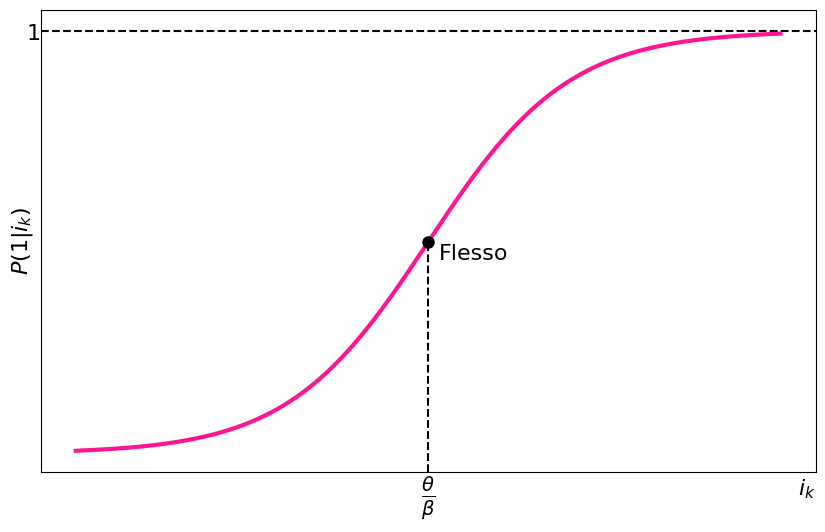
\includegraphics[width=0.6\textwidth]{pics/16_1.png} % INSERIRE QUI IL PERCORSO DEL GRAFICO
\caption{La probabilità che un fotone sia stato assorbito, data la corrente $i_k$.}
\label{fig:ch16_1}
\end{figure}

Quindi, il filtro ottimale diventa:

\begin{equation} \label{eq:ch16_12}
n_{ext}^{opt}(\{i_k\}) = \sum_{k=1}^{N} P(1 | i_k) = \sum_{k=1}^{N} \frac{1}{1 + e^{\theta_k - \beta i_k}}
\end{equation}

Questo risultato mostra che il filtro ottimale non è una semplice somma lineare delle correnti $i_k$. Ogni corrente $i_k$ viene pesata da un fattore non lineare $P(1|i_k)$ che dipende dalla corrente stessa. Le correnti che sono molto probabilmente dovute al rumore (cioè $i_k$ piccole in modulo, o comunque tali che $P(1|i_k) \approx 0$) contribuiscono poco alla somma, mentre quelle che sono molto probabilmente dovute all'assorbimento di un fotone ($P(1|i_k) \approx 1$) contribuiscono pienamente. Questo implementa un meccanismo di "noise gating" o filtraggio non lineare che migliora il rapporto segnale/rumore rispetto alla semplice somma lineare.

\begin{figure}[h!]
\centering
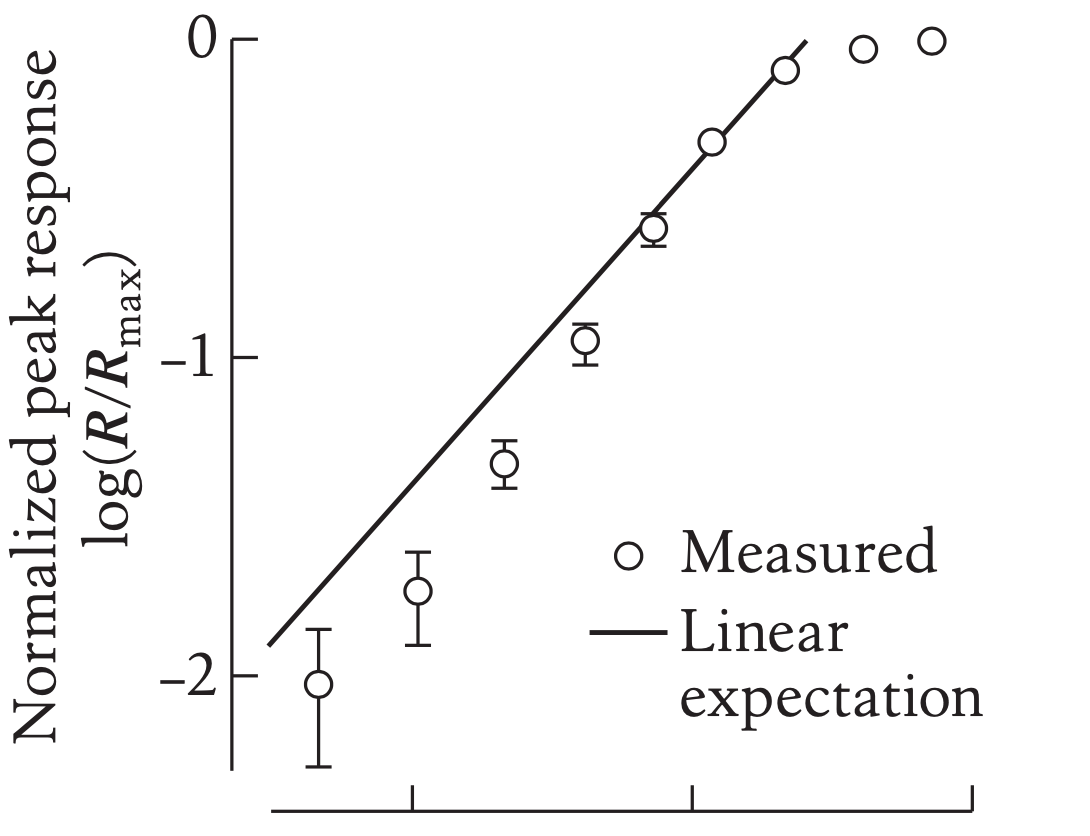
\includegraphics[width=0.6\textwidth]{pics/16_2.png} % INSERIRE QUI IL PERCORSO DEL GRAFICO
\caption{Ampiezze delle risposte di corrente (normalizzate al valore massimo) in funzione dell'intensità dello stimolo (in unità di $I_{1/2}$) (grafico log-log).}
\label{fig:ch16_2}
\end{figure}

L’andamento sperimentale è chiaramente non lineare.


\section{Modello di Ising}

Il modello di Ising rappresenta un sistema archetipico per lo studio dei comportamenti collettivi in fisica.
In questo modello, si considera un reticolo; su ogni sito reticolare è definita una variabile identificata come il momento magnetico individuale di spin dell'atomo situato sul sito. Tale variabile, denominata spin $s_i$, può assumere esclusivamente due valori:

\begin{itemize}
    \item $s_i = -1$: corrispondente a un momento magnetico di spin orientato verso il basso.
    \item $s_i = +1$: corrispondente a un momento magnetico di spin orientato verso l'alto.
\end{itemize}

\subsection*{Hamiltoniana del Modello di Ising}
L'energia del sistema, descritta dalla funzione Hamiltoniana $H$, è espressa come:

\begin{equation} \label{eq:ch16_13}
H = -\sum_{\langle i,j \rangle} J_{ij} s_i s_j - \sum_i h_i s_i 
\end{equation}

dove la somma $\langle i,j \rangle$ è ristretta alle coppie di primi vicini.

Il primo termine rappresenta l'interazione tra spin, o termine di allineamento.
$J_{ij}$ è una matrice che definisce quali coppie di spin interagiscono e l'intensità di tale interazione. Se $J_{ij} = 0$ per una specifica coppia di siti $i$ e $j$, gli spin localizzati su tali siti non interagiscono tra loro.
Si considera il caso in cui $J_{ij} = J > 0$ se i siti $i$ e $j$ sono primi vicini. Questa configurazione è nota come interazione a primi vicini. La definizione di "primi vicini" e il loro numero dipendono dalla geometria e dalla dimensionalità del reticolo.
Con $J > 0$, l'interazione è di tipo ferromagnetico e favorisce l'allineamento parallelo degli spin. Per minimizzare l'energia, il prodotto $s_i s_j$ deve essere positivo, il che implica che $s_i$ e $s_j$ abbiano lo stesso segno. Questo termine è detto di allineamento poiché la minimizzazione dell'energia si ottiene allineando gli spin.
Il secondo termine descrive l'interazione con un campo magnetico esterno $h_i$. Un campo magnetico esterno tende ad allineare gli spin parallelamente alla propria direzione.
In presenza di un campo magnetico, si manifestano due effetti competitivi: l'effetto del campo magnetico, che tende ad allineare ciascun spin a sé stesso, e l'effetto dell'interazione, per cui ciascun spin tende ad allinearsi con i propri vicini.
Questo modello è generalizzabile a sistemi non fisici, come quelli sociali, biologici o economici, in cui si osservano tendenze imitative (corrispondenti al termine di allineamento) e risposte a stimoli esterni (analoghi al campo magnetico).

\subsection*{Meccanica Statistica del Sistema}
Per l'analisi della meccanica statistica del sistema a una data temperatura, in equilibrio con un bagno termico, si impiega l'ensemble canonico. La quantità centrale da calcolare è la funzione di partizione $Z$.
Denotando con $S = \{s_1, s_2, \dots, s_N\}$ l'insieme di tutte le configurazioni di spin, la funzione di partizione è definita come:

\begin{equation} \label{eq:ch16_14}
Z = \sum_S e^{-\beta H(S)} 
\end{equation}

dove $\beta = 1/(k_B T)$, con $k_B$ costante di Boltzmann. La somma si estende a tutte le possibili configurazioni di spin $S$.
Ottenuta $Z$, si può determinare la misura di Boltzmann, ovvero la probabilità $P(S)$ associata a ciascuna configurazione di spin:

\begin{equation} \label{eq:ch16_15}
P(S) = \frac{1}{Z} e^{-\beta H(S)} 
\end{equation}

Utilizzando questa distribuzione di probabilità, è possibile calcolare il valore medio di qualsiasi osservabile, le sue fluttuazioni e altre grandezze termodinamiche.

\textbf{Energia Media:}
Il valore medio dell'energia $\langle E \rangle$ è dato da:

\begin{equation} \label{eq:ch16_16}
\langle E \rangle = \sum_S H(S) P(S) = \frac{1}{Z} \sum_S H(S) \; e^{-\beta H(S)} 
\end{equation}

Analogamente, per il valor medio del quadrato dell'energia, $\langle E^2 \rangle$:

\begin{equation} \label{eq:ch16_17}
\langle E^2 \rangle = \frac{1}{Z} \sum_S H(S)^2 e^{-\beta H(S)} 
\end{equation}

\textbf{Media di un'Osservabile Generica:}
Per una generica osservabile $O(S)$, il suo valore medio è:

\begin{equation} \label{eq:ch16_18}
\langle O \rangle = \sum_S O(S) P(S) = \frac{1}{Z} \sum_S O(S) e^{-\beta H(S)} 
\end{equation}

Una volta nota la funzione di partizione $Z$, è possibile derivare l'energia libera, l'entropia e altre funzioni di stato.

\subsection*{Analisi del Comportamento del Sistema}
Per semplicità, consideriamo inizialmente il caso senza campo esterno ($H_{ext} = 0$).

\begin{equation} \label{eq:ch16_19}
H = -J \sum_{\langle i,j \rangle} S_i S_j
\end{equation}

Questo modello descrive un comportamento puramente allelomimetico, ovvero di imitazione, molto comune nei sistemi biologici: ogni spin "vuole" essere simile ai suoi vicini.
Due fattori principali influenzano il sistema:
\begin{itemize}
    \item \textbf{a) L'ambiente (Temperatura):} L'ambiente introduce rumore nel sistema. In fisica statistica, questo rumore è modellato dalla temperatura $T$. Una temperatura elevata corrisponde a un grande rumore esterno, che tende a randomizzare l'orientamento degli spin, favorendo il disordine (aumento dell'entropia). Questo ambiente è detto bagno termico, ma può rappresentare qualsiasi fonte di rumore, come le perturbazioni ambientali per uno stormo di uccelli.
    \item \textbf{b) L'interazione:} L'interazione, rappresentata dal termine con $J$, si oppone al disordine e favorisce l'allineamento di tutti gli spin.
\end{itemize}

Analizziamo i casi estremi:

\subsubsection*{1) Caso a Temperatura Zero}
A $T=0$, il sistema cerca di raggiungere lo stato di energia minima. L'energia è minimizzata quando tutti gli spin sono allineati. Assumiamo che siano tutti orientati verso l'alto ($S_i = +1$ per ogni $i$).
L'energia di interazione si calcola sommando su tutte le coppie di primi vicini. Il numero di primi vicini di un sito è indicato con $z$ (es. su un reticolo quadrato, $z=4$).
L'energia minima del sistema sarà:

\begin{equation} \label{eq:ch16_20}
H_{min} = -J \frac{Nz}{2}
\end{equation}

Il fattore $1/2$ evita di contare due volte ogni coppia.
Esistono due stati che corrispondono a questa energia minima: quello con tutti gli spin up e quello con tutti gli spin down. Questo avviene perché l'Hamiltoniana possiede una simmetria di inversione degli spin: se invertiamo tutti gli spin di una qualsiasi configurazione, otteniamo una nuova configurazione con la stessa identica energia. Di conseguenza, anche lo stato di energia minima deve avere il suo "gemello" con spin invertiti. In questa condizione il sistema è perfettamente ordinato.

\subsubsection*{2) Caso a Temperatura Infinita}
Quando $T \rightarrow \infty$, $\beta \rightarrow 0$. Il fattore di Boltzmann $e^{-\beta H(S)}$ tende a 1 per qualsiasi configurazione.

\begin{equation} \label{eq:ch16_21}
P(S) = \frac{e^{-\beta H(S)}}{Z} \approx \frac{1}{Z}
\end{equation}

Ciò significa che tutte le configurazioni diventano equiprobabili. In questa situazione, il contributo dominante alle grandezze termodinamiche proviene dall'entropia. I macrostati più probabili sono quelli disordinati, poiché possono essere realizzati in un numero molto maggiore di microstati. Ad esempio, una configurazione con metà spin up e metà spin down ($K=N/2$) può essere ottenuta in $\binom{N}{K}$ modi, che è il valore massimo del coefficiente binomiale. Al contrario, gli stati perfettamente ordinati (tutti up o tutti down) sono unici.
In questo limite, l'interazione diventa trascurabile. L'energia fornita dal bagno termico è così alta che ogni spin fluttua in modo casuale e indipendente dagli altri.

\subsection*{Parametro d'Ordine e Transizioni di Fase}
Una quantità media di particolare rilevanza è il parametro d'ordine, che caratterizza lo stato macroscopico del sistema. Per il modello di Ising, il parametro d'ordine usuale è la magnetizzazione $M$.
La magnetizzazione totale (non normalizzata) è:

\begin{equation} \label{eq:ch16_22}
M = \sum_i \langle s_i \rangle 
\end{equation}

La magnetizzazione intensiva $m$ (magnetizzazione per spin) è:

\begin{equation} \label{eq:ch16_23}
m = \frac{1}{N} \sum_i \langle s_i \rangle 
\end{equation}

Si osservano due regimi distinti:
\begin{itemize}
    \item Ad alta temperatura ($T \to \infty$), i termini entropici sono dominanti. Il rumore termico induce fluttuazioni aleatorie e intense degli spin, prevalendo sull'effetto di allineamento. Il sistema non presenta un allineamento globale, risultando in $m \approx 0$. Questa fase è detta paramagnetica.
    \item A bassa temperatura ($T \to 0$), il termine energetico è preponderante e favorisce l'allineamento degli spin. Il sistema acquisisce una magnetizzazione non nulla, $m \neq 0$. Questa fase è detta ferromagnetica.
\end{itemize}

Variando la temperatura da valori elevati verso valori bassi, si identifica una temperatura critica $T_c$ alla quale il sistema transisce dalla fase paramagnetica a quella ferromagnetica. Tale transizione è una transizione di fase.

\begin{figure}[h!]
\centering
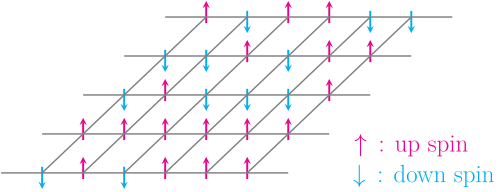
\includegraphics[width=0.6\textwidth]{pics/16_3.png} % INSERIRE QUI IL PERCORSO DEL GRAFICO DELLA MAGNETIZZAZIONE
\caption{Andamento della magnetizzazione $m$ in funzione della temperatura $T$.}
\label{fig:ch16_3}
\end{figure}

L'andamento di $m(T)$ mostra che:
\begin{itemize}
    \item $m=0$ per $T > T_c$
    \item $m \neq 0$ per $T < T_c$
\end{itemize}

Per $T < T_c$, il sistema manifesta un ordine ferromagnetico.

\vspace{0.5cm}
\noindent\fbox{%
    \parbox{\dimexpr\linewidth-2\fboxsep-2\fboxrule\relax}{%
        \textbf{!!}\\
        In assenza di un campo magnetico esterno ($h=0$), esistono due stati di equilibrio equivalenti: uno con tutti gli spin orientati verso l'alto ($m > 0$) e uno con tutti gli spin orientati verso il basso ($m < 0$).\\
        L'Hamiltoniana del sistema (con $h=0$) possiede una simmetria per inversione globale degli spin (cioè, $s_i \to -s_i$ per tutti gli $i$).\\
        Lo stato paramagnetico ($m=0$) è invariante rispetto a tale simmetria.\\
        Gli stati ferromagnetici ($m \neq 0$) rompono questa simmetria: l'inversione globale degli spin trasforma uno stato magnetizzato nell'altro, che è fisicamente distinto.\\
        Questo fenomeno è noto come rottura spontanea della simmetria. A livello macroscopico, il sistema può trovarsi in uno dei due stati di equilibrio distinti, ciascuno dei quali, singolarmente considerato, non possiede la piena simmetria dell'Hamiltoniana.
    }%
}
\vspace{0.5cm}

\subsection*{Approssimazione di Campo Medio (Mean Field)}
Risolvere esattamente il modello di Ising è un problema complesso. Per ottenere una comprensione qualitativa, si utilizza l'approssimazione di campo medio. L'idea è trasformare il sistema interagente in un sistema non interagente efficace.
Partiamo dall'Hamiltoniana completa con un campo esterno omogeneo $h$:

\begin{equation} \label{eq:ch16_24}
H = -J \sum_{\langle i,j \rangle} S_i S_j - h \sum_i S_i
\end{equation}

Il termine di interazione $\sum S_i S_j$ rende il problema difficile. L'approssimazione consiste nel riscrivere ogni spin $S_i$ come la somma del suo valore medio $m$ e di una fluttuazione $\delta S_i$:

\begin{equation} \label{eq:ch16_25}
S_i = \langle S_i \rangle + (S_i - \langle S_i \rangle) = m + \delta S_i
\end{equation}

Dato che il campo $h$ è omogeneo, il valore medio $\langle S_i \rangle$ è lo stesso per tutti i siti, $m_i = m$.
Sostituendo questa espressione nel termine di interazione:

\begin{equation} \label{eq:ch16_26}
S_i S_j = (m + \delta S_i)(m + \delta S_j) = m^2 + m(\delta S_i + \delta S_j) + \delta S_i \delta S_j
\end{equation}

Finora non abbiamo fatto alcuna approssimazione.
Il termine $\delta S_i \delta S_j$ accoppia le fluttuazioni degli spin sui siti $i$ e $j$. Questa è la parte più interessante e complessa, poiché descrive come gli spin tendano a fluttuare in modo coordinato.

\vspace{0.5cm}
\noindent\fbox{%
    \parbox{\dimexpr\linewidth-2\fboxsep-2\fboxrule\relax}{%
        L'approssimazione di campo medio consiste nel trascurare questo termine:
        \begin{equation} \label{eq:ch16_27}
        \delta S_i \delta S_j \approx 0
        \end{equation}
    }%
}
\vspace{0.5cm}

Fisicamente, questo equivale a dire che le fluttuazioni degli spin non sono correlate. Ogni spin non "vede" più le fluttuazioni istantanee dei suoi vicini, ma solo il loro effetto medio, rappresentato da $m$.
Con questa approssimazione, il termine di interazione nell'Hamiltoniana diventa:

\begin{equation} \label{eq:ch16_28}
\sum_{\langle i,j \rangle} S_i S_j \approx \frac{1}{2} \sum_{i \neq j} m_{ij} (m^2 + m\delta S_i + m\delta S_j)
\end{equation}

Dove $m_{ij}$ è la matrice di connettività (dice se due spin interagiscono).
Analizziamo i termini separatamente:

\textbf{Termine costante:}
\begin{equation} \label{eq:ch16_29}
\frac{1}{2} \sum_{i \neq j} m_{ij} m^2 = \frac{m^2}{2} \sum_{i} \sum_{j \neq i} m_{ij} = \frac{m^2}{2} \sum_{i} z = \frac{m^2 N z}{2}
\end{equation}

\textbf{Termini lineari nelle fluttuazioni:}
\begin{equation} \label{eq:ch16_30}
\frac{1}{2} \sum_{i \neq j} m_{ij} (m\delta S_i + m\delta S_j) = m \sum_{i \neq j} m_{ij} \delta S_j
\end{equation}

Ricordando che $\delta S_j = S_j - m$:

\begin{align}
m \sum_{i \neq j} m_{ij} (S_j - m) &= m \sum_j \left( \sum_{i \neq j} m_{ij} \right) S_j - m^2 \sum_{i \neq j} m_{ij} \nonumber \\  &= m z \sum_j S_j - m^2 N z \label{eq:ch16_31}
\end{align}

Mettendo insieme tutti i pezzi del termine di interazione approssimato:

\begin{equation} \label{eq:ch16_32}
\sum_{\langle i,j \rangle} m_{ij} S_i S_j \approx \frac{m^2 N z}{2} + m z \sum_j S_j - m^2 N z = - \frac{m^2 N z}{2} + m z \sum_j S_j
\end{equation}

Sostituendo questo risultato nell'Hamiltoniana, otteniamo l'Hamiltoniana di campo medio $H_{MF}$:

\begin{equation} \label{eq:ch16_33}
H_{MF} \approx -J \left( - \frac{m^2 N z}{2} + m z \sum_i S_i \right) - h \sum_i S_i
\end{equation}

Raggruppando i termini:

\begin{equation} \label{eq:ch16_34}
H_{MF} \approx \frac{J N z m^2}{2} - (h + J z m) \sum_i S_i
\end{equation}

Questa Hamiltoniana descrive un sistema di spin non interagenti. Il primo termine è una costante energetica, mentre il secondo mostra che ogni spin $S_i$ è soggetto a un campo efficace $h_{eff}$:

\begin{equation} \label{eq:ch16_35}
h_{eff} = h + J z m
\end{equation}

Questo campo efficace è la somma del campo esterno $h$ e del "campo molecolare" $Jzm$, che rappresenta l'influenza media di tutti i vicini sullo spin singolo.
Ora che il sistema è non interagente, possiamo calcolare facilmente la funzione di partizione.
La probabilità di una configurazione $S$ è:

\begin{equation} \label{eq:ch16_36}
P(S) = \frac{1}{Z} e^{-\beta H_{MF}(S)} = A \prod_i e^{\beta h_{eff} S_i} = \prod_i P(S_i)
\end{equation}

La probabilità si fattorizza, e la funzione di partizione totale $Z$ è il prodotto delle funzioni di partizione dei singoli spin, $Z = (Z_1)^N$. Calcoliamo $Z_1$ per un singolo spin, che ha Hamiltoniana $H_1 = -h_{eff}S_i$:

\begin{equation} \label{eq:ch16_37}
Z_1 = \sum_{S_i = \pm 1} e^{-\beta H_1(S_i)} = e^{\beta h_{eff}(+1)} + e^{\beta h_{eff}(-1)} = 2 \cosh(\beta h_{eff})
\end{equation}

\begin{equation} \label{eq:ch16_38}
Z_1 =  2 \cosh(\beta h_{eff})
\end{equation}

Infine, calcoliamo il valore medio di un singolo spin, che deve essere uguale alla magnetizzazione per sito $m$ che abbiamo introdotto all'inizio. Questa è la condizione di autocoerenza (self-consistency).

\begin{equation} \label{eq:ch16_39}
m  = \frac{1}{Z_1} \sum_{S_i = \pm 1} S_i e^{\beta h_{eff} S_i} = \frac{(+1)e^{\beta h_{eff}} + (-1)e^{-\beta h_{eff}}}{2 \cosh(\beta h_{eff})} = \frac{2 \sinh(\beta h_{eff})}{2 \cosh(\beta h_{eff})}
\end{equation}

\begin{equation} \label{eq:ch16_40}
m = \tanh(\beta h_{eff})
\end{equation}

Sostituendo l'espressione per $h_{eff}$, otteniamo l'equazione finale di autocoerenza per la magnetizzazione:

\begin{equation} \label{eq:ch16_41}
m = \tanh(\beta (h + Jzm))
\end{equation}

Questa equazione implicita lega la magnetizzazione $m$ a se stessa e ai parametri del sistema.

%-------------------------------------------------------------------------------
% CAPITOLO 17
%-------------------------------------------------------------------------------
\chapter{Lezione 17}
\label{capitolo_17}
\textit{29/04/2025}

\section{Forma generale del modello di Ising}
Il modello di Ising è un modello fondamentale in meccanica statistica. L'Hamiltoniana nella sua forma più generale, che descrive l'energia di una data configurazione di spin $\{S_i\}$, è data da:

\begin{equation} \label{eq:ch17_1}
H = -J \sum_{\langle i,j \rangle} S_i S_j - \sum_i h_i S_i
\end{equation}

Dove:
\begin{itemize}
    \item $S_i$ sono le variabili di spin, che possono assumere i valori $\pm 1$.
    \item La prima somma è estesa a tutte le coppie di spin primi vicini $\langle i,j \rangle$ su un reticolo.
    \item $J$ è la costante di accoppiamento. Se $J>0$, l'interazione è ferromagnetica e gli spin tendono ad allinearsi.
    \item $h_i$ è un campo magnetico esterno che può essere dipendente dal sito $i$.
\end{itemize}

Il termine di interazione può essere riscritto come $\frac{1}{2} \sum_{i \neq j} J_{ij} S_i S_j$, dove $J_{ij}$ è la matrice di interazione.

\section{Approssimazione di Campo Medio (Mean Field)}
Risolvere esattamente questo modello è complesso. Un'approssimazione potente è quella del campo medio. L'idea fisica è che ogni spin non interagisce con lo stato istantaneo dei suoi vicini, ma con il loro campo medio. Stiamo di fatto trascurando le correlazioni tra le fluttuazioni degli spin vicini.

Matematicamente, approssimiamo il termine di interazione:

\begin{equation} \label{eq:ch17_2}
\sum_{\langle i,j \rangle} S_i S_j = \frac{1}{2} \sum_i S_i \left( \sum_{j \in N(i)} S_j \right)
\end{equation}

Nell'approssimazione di campo medio, sostituiamo il valore istantaneo dello spin $S_j$ con il suo valore medio $\langle S_j \rangle$. Questo trasforma un termine fluttuante in uno che descrive l'interazione dello spin $S_i$ con un campo medio efficace generato dai suoi vicini.

L'Hamiltoniana di campo medio ($H_{mf}$) diventa:

\begin{equation} \label{eq:ch17_3}
H_{mf} = -\sum_i S_i h_i^{eff}
\end{equation}

Dove $h_i^{eff}$ è il campo efficace:

\begin{equation} \label{eq:ch17_4}
h_i^{eff} = h_i + J \sum_{j \in N(i)} \langle S_j \rangle
\end{equation}

Questo campo ha due contributi: il campo esterno $h_i$ e il campo medio generato dai vicini.

\subsection*{Caso Omogeneo}
Per semplificare, consideriamo il caso omogeneo in cui il campo esterno è uniforme ($h_i = h$ per ogni $i$) e, per simmetria, la magnetizzazione locale media è la stessa per ogni sito ($\langle S_j \rangle = m$). Se $z$ è il numero di primi vicini, il campo efficace diventa:

\begin{equation} \label{eq:ch17_5}
h^{eff} = h + zJm
\end{equation}

Durante la derivazione dell'Hamiltoniana di campo medio, appare anche un termine aggiuntivo che dipende da $m^2$. Questo termine è costante rispetto alle variabili di spin $\{S_i\}$ ed è cruciale quando si calcola la probabilità di una specifica magnetizzazione $m$. L'Hamiltoniana completa in questa approssimazione è:

\vspace{0.5cm}
\noindent\fbox{%
    \parbox{\dimexpr\linewidth-2\fboxsep-2\fboxrule\relax}{%
        \begin{equation} \label{eq:ch17_6}
        H_{MF} = -h^{eff} \sum_i S_i + \frac{N z J m^2}{2}
        \end{equation}
    }%
}
\vspace{0.5cm}

\subsection*{Fattorizzazione della Misura di Probabilità}
Un risultato fondamentale dell'approssimazione di campo medio è che l'Hamiltoniana è una somma di termini che dipendono da un singolo spin, $H_{mf} = \sum_i H_i(S_i)$.
Di conseguenza, la probabilità per una configurazione $\{S_i\}$ si fattorizza:

\begin{equation} \label{eq:ch17_7}
P(\{S_i\}) = \frac{e^{-\beta H_{mf}}}{Z} = \prod_{i=1}^N \frac{e^{-\beta H_i(S_i)}}{Z_1} = \prod_{i=1}^N P(S_i)
\end{equation}

Questo significa che gli spin diventano indipendenti e possiamo analizzare un singolo sito alla volta. La funzione di partizione per un singolo spin è:

\begin{equation} \label{eq:ch17_8}
Z_{1} = \sum_{S_i = \pm 1} e^{\beta h^{eff} S_i} = 2 \cosh(\beta h^{eff})
\end{equation}

\subsection*{Equazione di Autoconsistenza per la Magnetizzazione}
La magnetizzazione media per sito, $m$, è definita come $m = \langle S_i \rangle$. La calcoliamo usando la distribuzione di probabilità per un singolo spin:

\begin{equation} \label{eq:ch17_9}
m = \langle S_i \rangle = \frac{\sum_{S_i=\pm 1} S_i e^{\beta h^{eff} S_i}}{\sum_{S_i=\pm 1} e^{\beta h^{eff} S_i}} = \tanh(\beta h^{eff})
\end{equation}

Questa è un'equazione per la magnetizzazione. Sostituendo l'espressione di $h^{eff}$, otteniamo l'equazione di autoconsistenza che dobbiamo risolvere per trovare $m$:

\begin{equation} \label{eq:ch17_10}
m = \tanh(\beta h + \beta z J m)
\end{equation}

\section{Soluzione in approssimazione di Campo Medio}

\subsection*{Caso 1: $J = 0$ (Nessuna Interazione)}
Se non ci sono interazioni ($J=0$), l'approssimazione di campo medio è esatta. L'equazione diventa:

\begin{equation} \label{eq:ch17_11}
m = \tanh(\beta h)
\end{equation}

In questo caso, la soluzione per $m$ è esplicita. Graficamente, la magnetizzazione $m$ in funzione di $\beta h$ è una curva "smooth", senza discontinuità.
Questo scenario non presenta transizioni di fase. Il sistema si allinea gradualmente con il campo esterno, e l'allineamento è contrastato dal rumore termico (la temperatura $T$). L'ordine è indotto dal campo esterno.

\begin{figure}[h!]
\centering
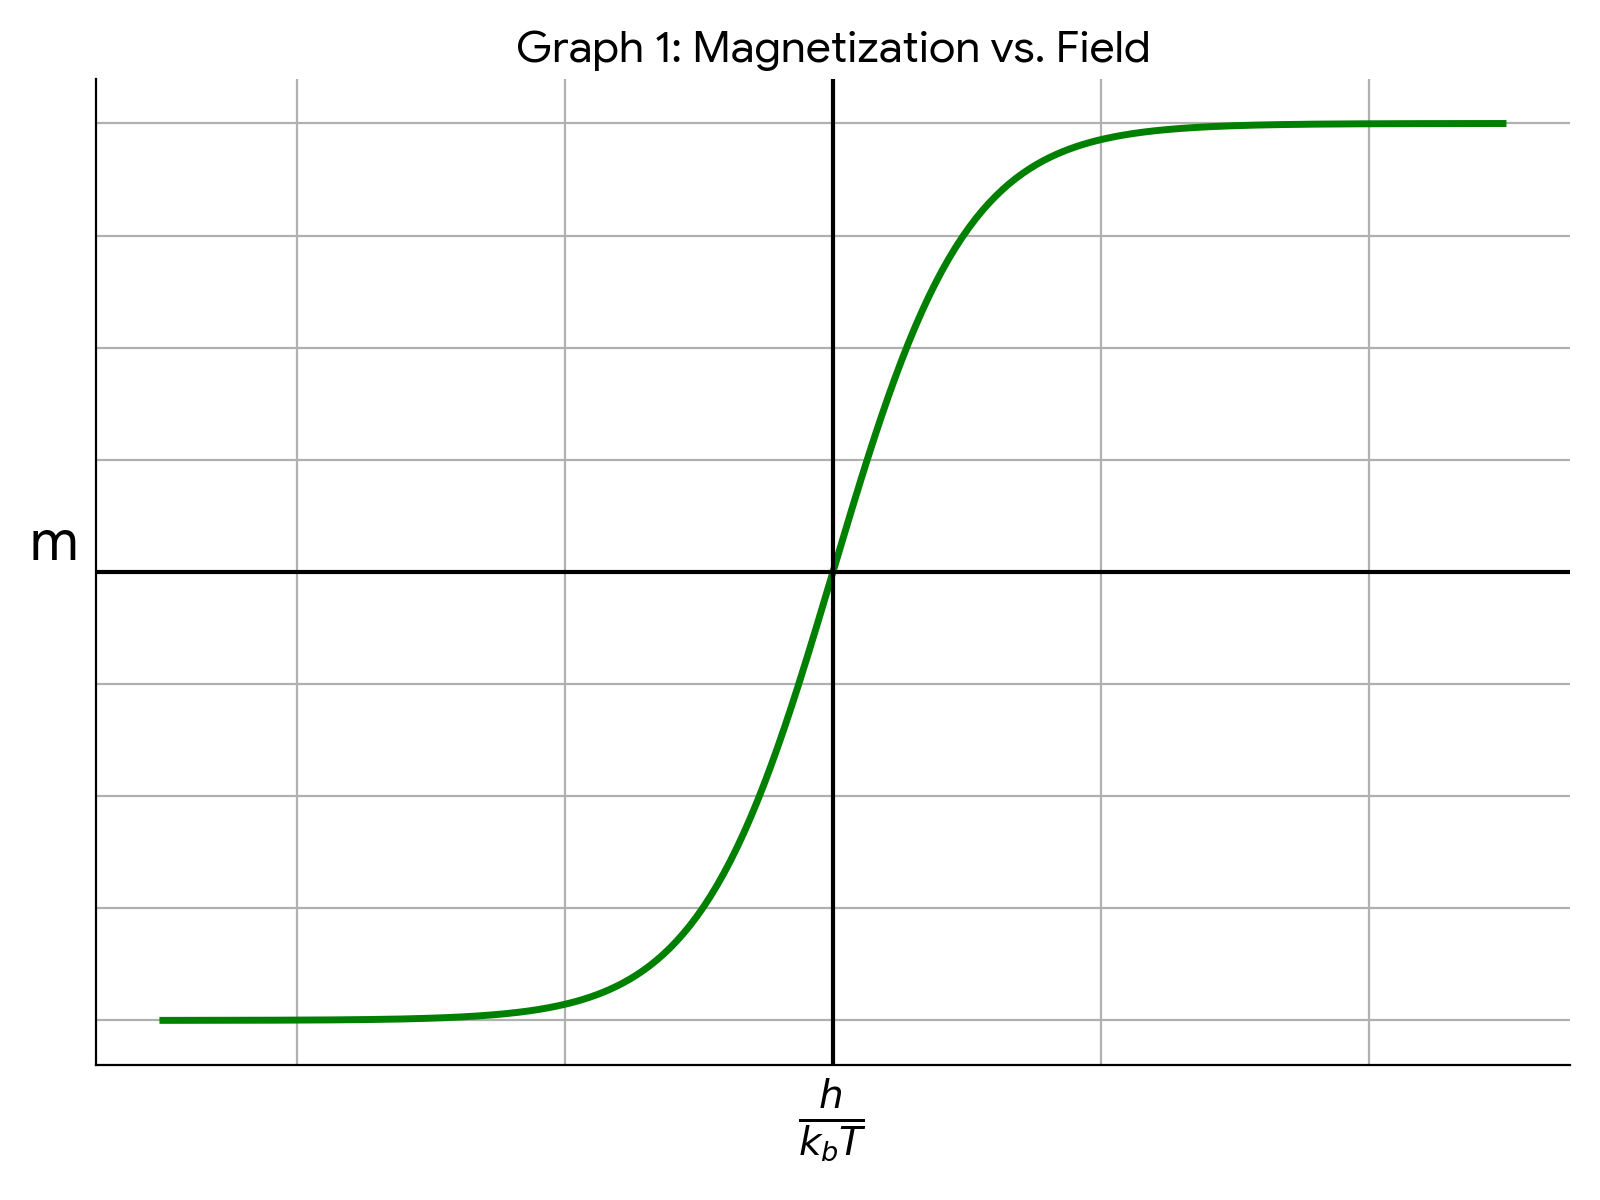
\includegraphics[width=0.6\textwidth]{pics/17_1.png} % INSERIRE QUI IL PERCORSO DEL GRAFICO
\caption{Andamento della magnetizzazione $m$ in funzione di $\beta h$ per $J=0$.}
\label{fig:ch17_1}
\end{figure}

\subsection*{Caso 2: $h = 0$, $J > 0$ (Interazioni senza Campo Esterno)}
Risolviamo l'equazione graficamente. Cerchiamo le intersezioni tra le due curve:
\begin{itemize}
    \item $y_1 = m$ (una retta con pendenza 1)
    \item $y_2 = \tanh(\beta z J m)$ (una tangente iperbolica)
\end{itemize}

La pendenza della tangente iperbolica nell'origine ($m=0$) è $\beta z J$. Il comportamento del sistema dipende dal confronto tra questa pendenza e la pendenza di $y_1$.

\subsubsection*{Alta Temperatura: $T > T_c$}
Se la temperatura è alta, $\beta$ è piccolo, quindi $\beta z J < 1$.
La pendenza della tangente iperbolica all'origine è minore di 1.
C'è solo un'intersezione in $m=0$. La magnetizzazione di equilibrio è nulla; il sistema è disordinato perché il rumore termico domina sull'interazione.

\begin{figure}[h!]
\centering
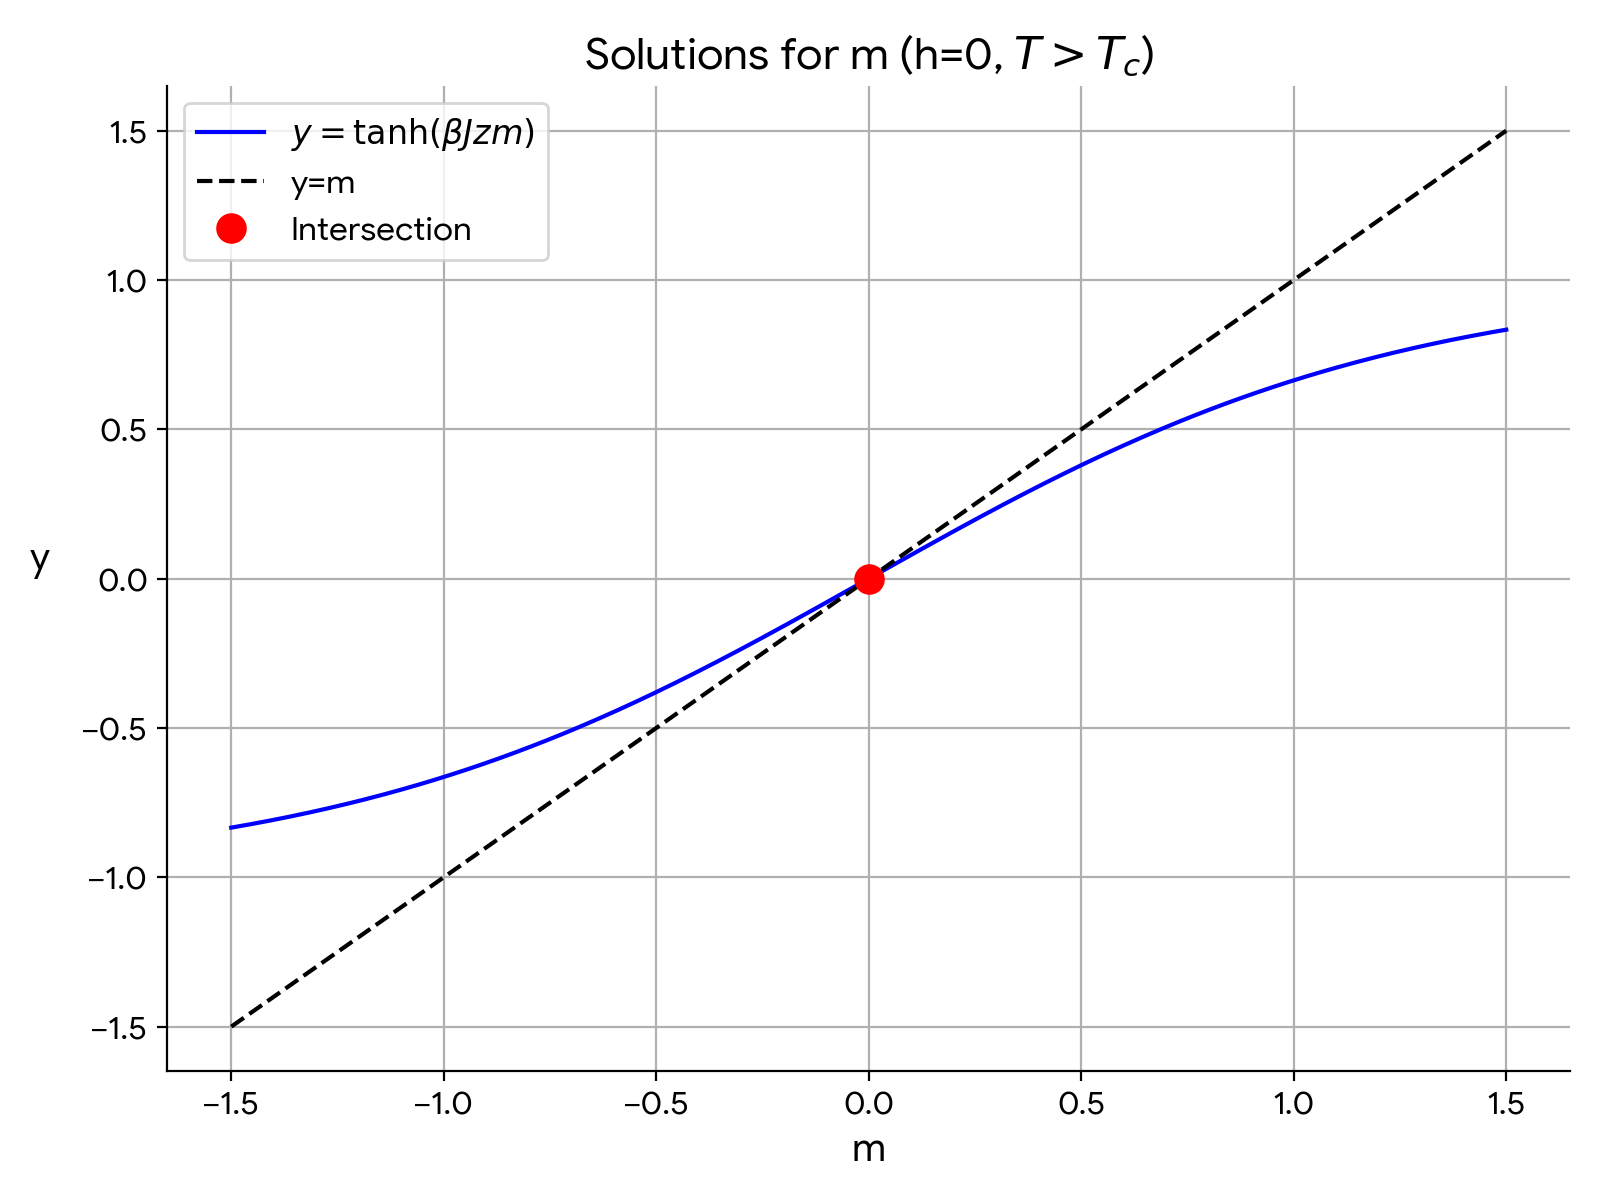
\includegraphics[width=0.6\textwidth]{pics/17_2.png} % INSERIRE QUI IL PERCORSO DEL GRAFICO
\caption{Soluzione per $T > T_c$.}
\label{fig:ch17_2}
\end{figure}

\subsubsection*{Temperatura Critica: $T = T_c$}
Esiste una temperatura critica $T_c$ tale che $\beta_c z J = 1$. Questo definisce la temperatura critica:

\begin{equation} \label{eq:ch17_12}
T_c = \frac{zJ}{k_B}
\end{equation}

A $T=T_c$, la pendenza della tangente iperbolica all'origine è esattamente 1. Anche in questo caso, l'unica soluzione è $m=0$.

\begin{figure}[h!]
\centering
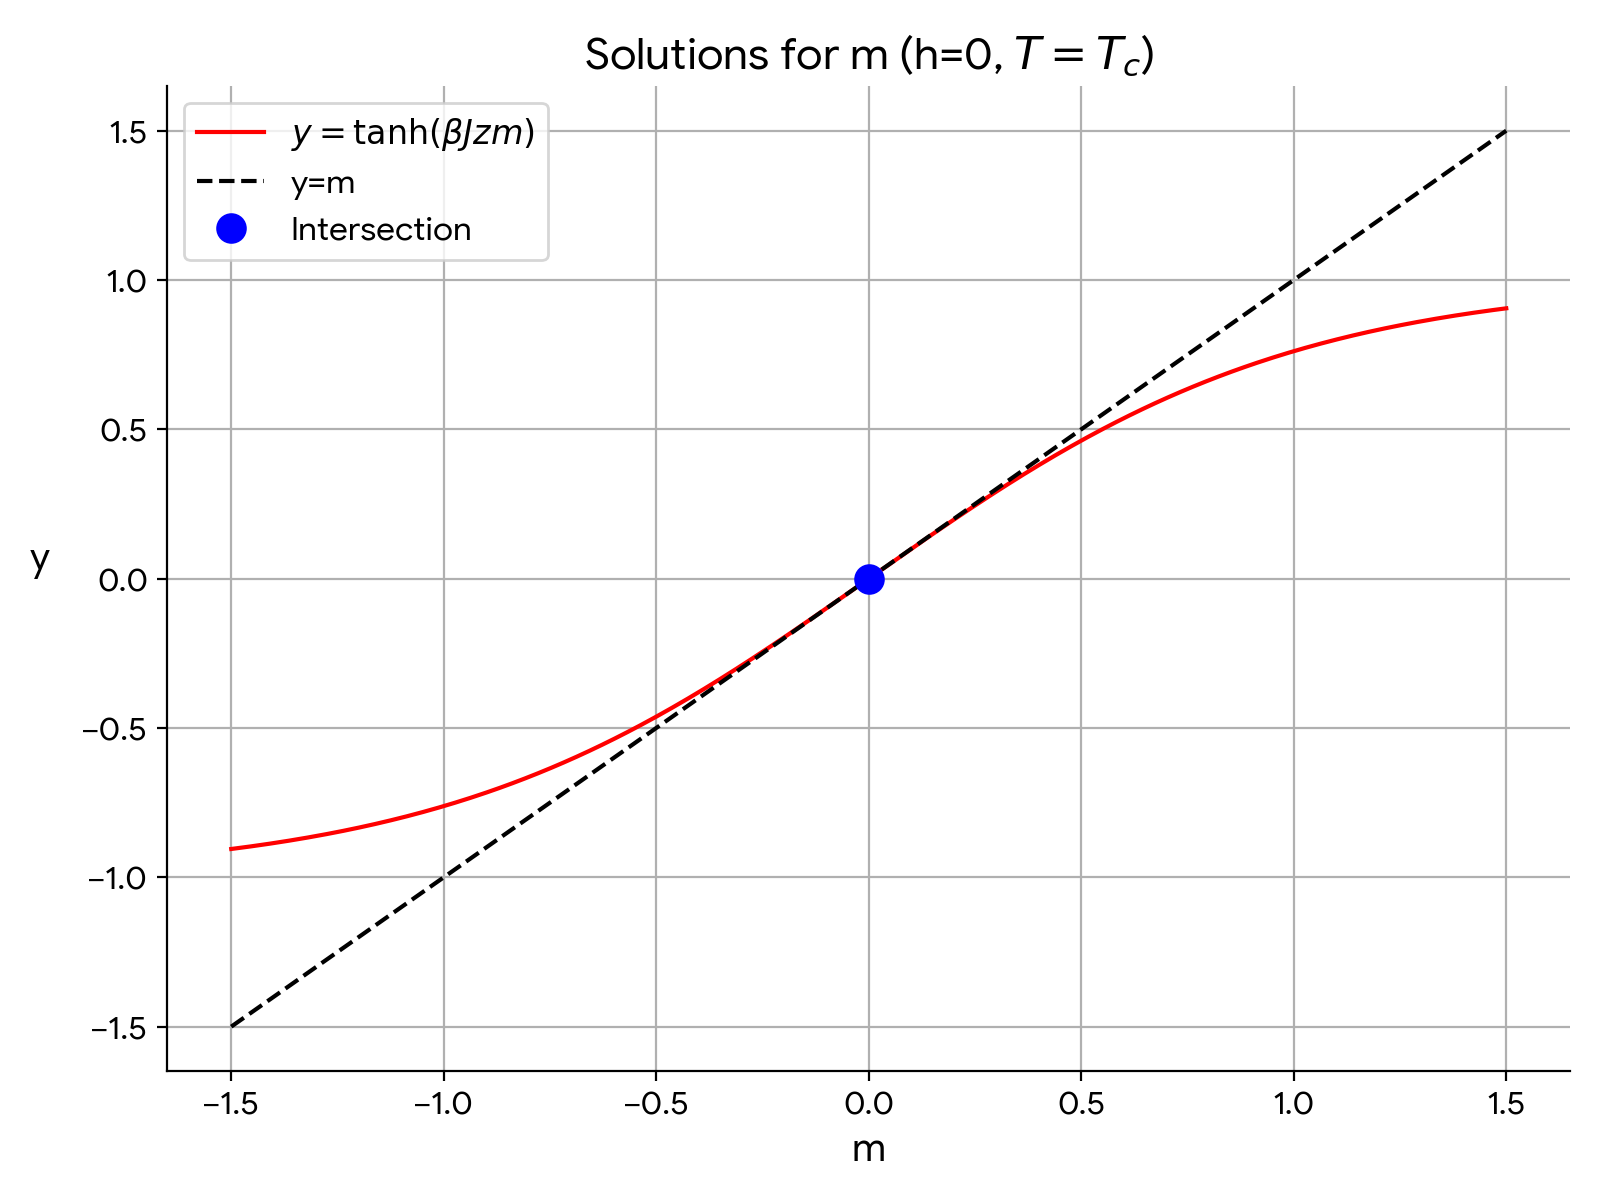
\includegraphics[width=0.6\textwidth]{pics/17_3.png} % INSERIRE QUI IL PERCORSO DEL GRAFICO
\caption{Soluzione per $T = T_c$.}
\label{fig:ch17_3}
\end{figure}

\subsubsection*{Bassa Temperatura: $T < T_c$}
Se $T < T_c$, allora $\beta z J > 1$. La pendenza della tangente iperbolica all'origine è maggiore di 1.
In questo caso, oltre alla soluzione $m=0$, compaiono altre due soluzioni simmetriche, $m^+$ e $m^-$.
La soluzione $m=0$ è instabile, mentre le soluzioni $m^\pm$ sono stabili. Il sistema sceglie spontaneamente una di queste due magnetizzazioni non nulle.

\begin{figure}[h!]
\centering
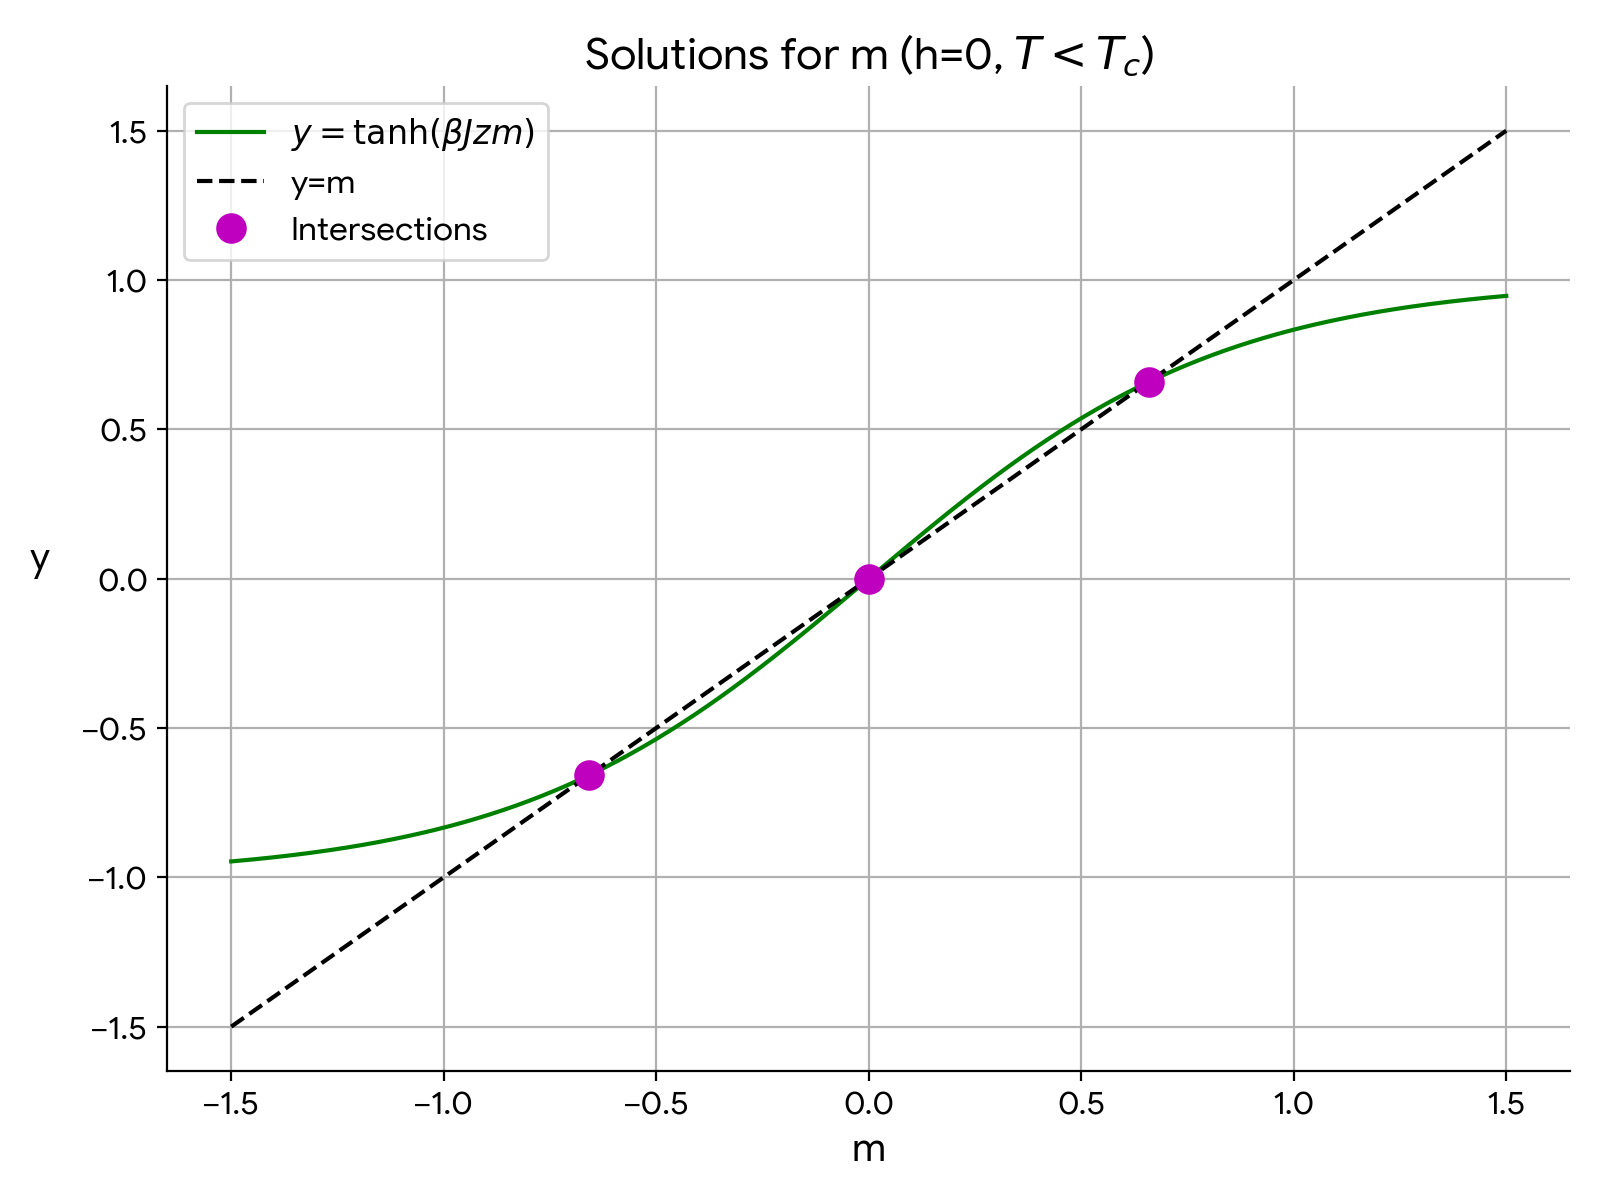
\includegraphics[width=0.6\textwidth]{pics/17_4.png} % INSERIRE QUI IL PERCORSO DEL GRAFICO
\caption{Soluzione per $T < T_c$.}
\label{fig:ch17_4}
\end{figure}

Il diagramma di $m$ in funzione di $T$ mostra che per $T>T_c$, $m=0$. A $T=T_c$, la soluzione si biforca, e per $T<T_c$ appaiono due rami di soluzioni stabili $m^\pm$.

\begin{figure}[h!]
\centering
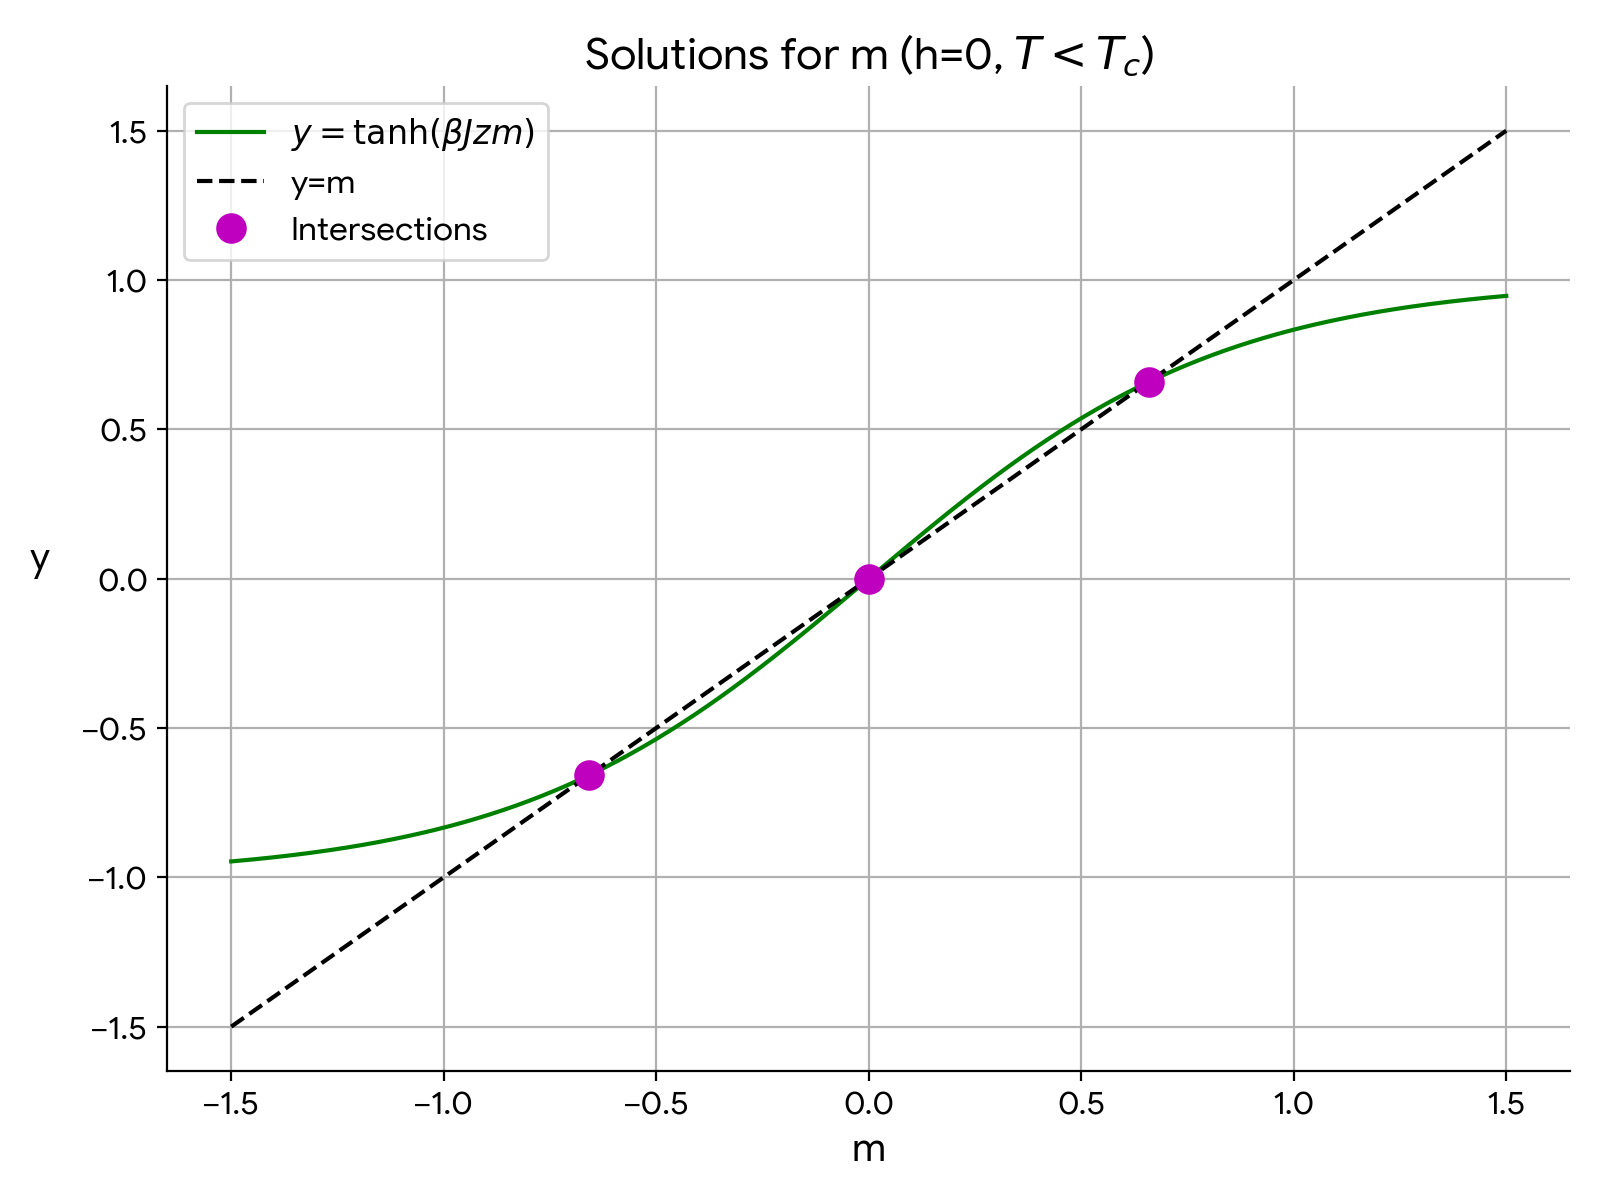
\includegraphics[width=0.6\textwidth]{pics/17_4.png} % INSERIRE QUI IL PERCORSO DEL GRAFICO DELLA BIFORCAZIONE
\caption{Diagramma di biforcazione della magnetizzazione $m$ in funzione della temperatura $T$.}
\label{fig:ch17_5}
\end{figure}


\section{Dalla Magnetizzazione alla Distribuzione di Probabilità}
La soluzione dell'equazione di autoconsistenza fornisce la magnetizzazione di equilibrio $m_{eq}$, ovvero il valore che misureremmo in un esperimento macroscopico. Tuttavia, su scale di tempo microscopiche, la magnetizzazione istantanea $m = \frac{1}{N} \sum_i S_i$ fluttua.
Vogliamo calcolare la distribuzione di probabilità $P(m)$ per questi valori istantanei.

Formalmente, si calcola sommando le probabilità di tutte le microconfigurazioni $\{S_i\}$ che corrispondono a un dato valore di $m$:

\begin{equation} \label{eq:ch17_13}
P\left(m = \frac{1}{N}\sum_i s_i\right) = \sum_{\{s_i\}} P(\{s_i\}) \delta\left(m - \frac{1}{N}\sum_i s_i\right)
\end{equation}

Sostituendo la probabilità di campo medio $P(\{s_i\}) \propto e^{-\beta H_{mf}}$ e usando la delta di Dirac per sostituire $\sum_i s_i = Nm$, l'espressione diventa:

\begin{equation} \label{eq:ch17_14}
P(m) = \frac{1}{Z_{TOT}} \sum_{\{s_i\}} e^{\beta h^{eff} (Nm) - \beta \frac{J N z m^2}{2}} \delta\left(m - \frac{1}{N}\sum_i s_i\right)
\end{equation}

L'obiettivo è scrivere questa probabilità nella forma $P(m) \propto e^{-\beta N f_{eff}(m)}$, dove $f_{eff}(m)$ è un'energia libera efficace. Per farlo, dobbiamo calcolare il termine entropico, ovvero la somma $\sum_{\{s_i\}} \delta(\dots)$, che conta il numero di configurazioni con magnetizzazione $m$.

Introduciamo il numero di spin "up" ($N^+$) e "down" ($N^-$):

\begin{equation} \label{eq:ch17_15}
M = \sum_i s_i = Nm = N^+ - N^-
\end{equation}
\begin{equation} \label{eq:ch17_16}
N = N^+ + N^-
\end{equation}

Risolvendo per $N^+$ e $N^-$:

\begin{equation} \label{eq:ch17_17}
N^+ = \frac{N(m+1)}{2} \quad , \quad N^- = \frac{N(1-m)}{2}
\end{equation}

Il numero di modi per arrangiare $N^+$ spin up e $N^-$ spin down su $N$ siti è dato dal coefficiente binomiale $\binom{N}{N^+}$. Usando l'approssimazione di Stirling ($\ln k! \approx k \ln k - k$) per $N$ grande, il suo logaritmo è:

\begin{equation} \label{eq:ch17_18}
\ln \binom{N}{N^+} = \ln N! - \ln N^+! - \ln N^-! \approx N\ln N - N^+\ln N^+ - N^-\ln N^-
\end{equation}

Sostituendo il termine entropico (espresso come $e^{\ln \binom{N}{N^+}}$) in $P(m)$, l'esponente completo diventa:

\begin{equation} \label{eq:ch17_19}
N\beta h^{eff}m - \beta \frac{J N z m^2}{2} + N\ln N - N^+\ln N^+ - N^-\ln N^-
\end{equation}

Sostituendo le espressioni di $N^+$ e $N^-$ in funzione di $m$ nei termini logaritmici e semplificando, i termini in $N\ln N$ si cancellano e l'esponente diventa:

\begin{equation*}
N\beta h^{eff}m - \beta \frac{J N z m^2}{2} - N\frac{1+m}{2}\ln(1+m) - N\frac{1-m}{2}\ln(1-m) + N\ln 2
\end{equation*}

Raccogliamo ora un fattore $-\beta N$ per identificare l'energia libera efficace $f_{eff}(m)$:

\begin{align} \label{eq:ch17_20}
P(m) &\propto \frac{1}{\mathcal{N}}\exp \left\{ -\beta N \left[ -mh^{eff} + \frac{J z m^2}{2} \right. \right. \nonumber\\ &\left. \left. + \frac{k_B T}{2} \left( (1+m)\ln(1+m) + (1-m)\ln(1-m) - 2\ln 2 \right) \right] \right\}
\end{align}

L'energia libera efficace per spin $f_{eff}(m)$ è l'espressione tra parentesi quadre. Trascurando la costante $-k_B T \ln 2$ (che viene assorbita nella normalizzazione), otteniamo:

\vspace{0.5cm}
\noindent\fbox{%
    \parbox{\dimexpr\linewidth-2\fboxsep-2\fboxrule\relax}{%
        \begin{equation*}
        f_{eff}(m) = -mh^{eff} + \frac{Jzm^2}{2} + \frac{k_B T}{2} [(1+m)\ln(1+m) + (1-m)\ln(1-m)]
        \end{equation*}
    }%
}
\vspace{0.5cm}


\section{Interpretazione di $f_{eff}(m)$}
Il valore di equilibrio della magnetizzazione, $m_{eq}$, corrisponde al valore $m^*$ che massimizza la probabilità $P(m)$. Per $N$ grande (metodo di Laplace), questo equivale a trovare il valore di $m$ che minimizza l'energia libera efficace $f_{eff}(m)$. Per trovare i minimi, poniamo la derivata uguale a zero:

\begin{equation} \label{eq:ch17_21}
\frac{d}{dm}f_{eff}(m) = 0
\end{equation}

Svolgendo la derivata, si ritrova esattamente l'equazione di autoconsistenza, mostrando la coerenza dell'approccio:

\begin{equation} \label{eq:ch17_22}
m = \tanh(\beta h_{eff}) = \tanh(\beta h + \beta z J m)
\end{equation}

L'analisi di $f_{eff}(m)$ conferma i risultati della soluzione grafica e permette di determinare la stabilità delle soluzioni.
Per $h=0$:
\begin{itemize}
    \item \textbf{$T > T_c$}: $f_{eff}(m)$ ha un solo minimo in $m=0$.
    \begin{figure}[h!]
\centering
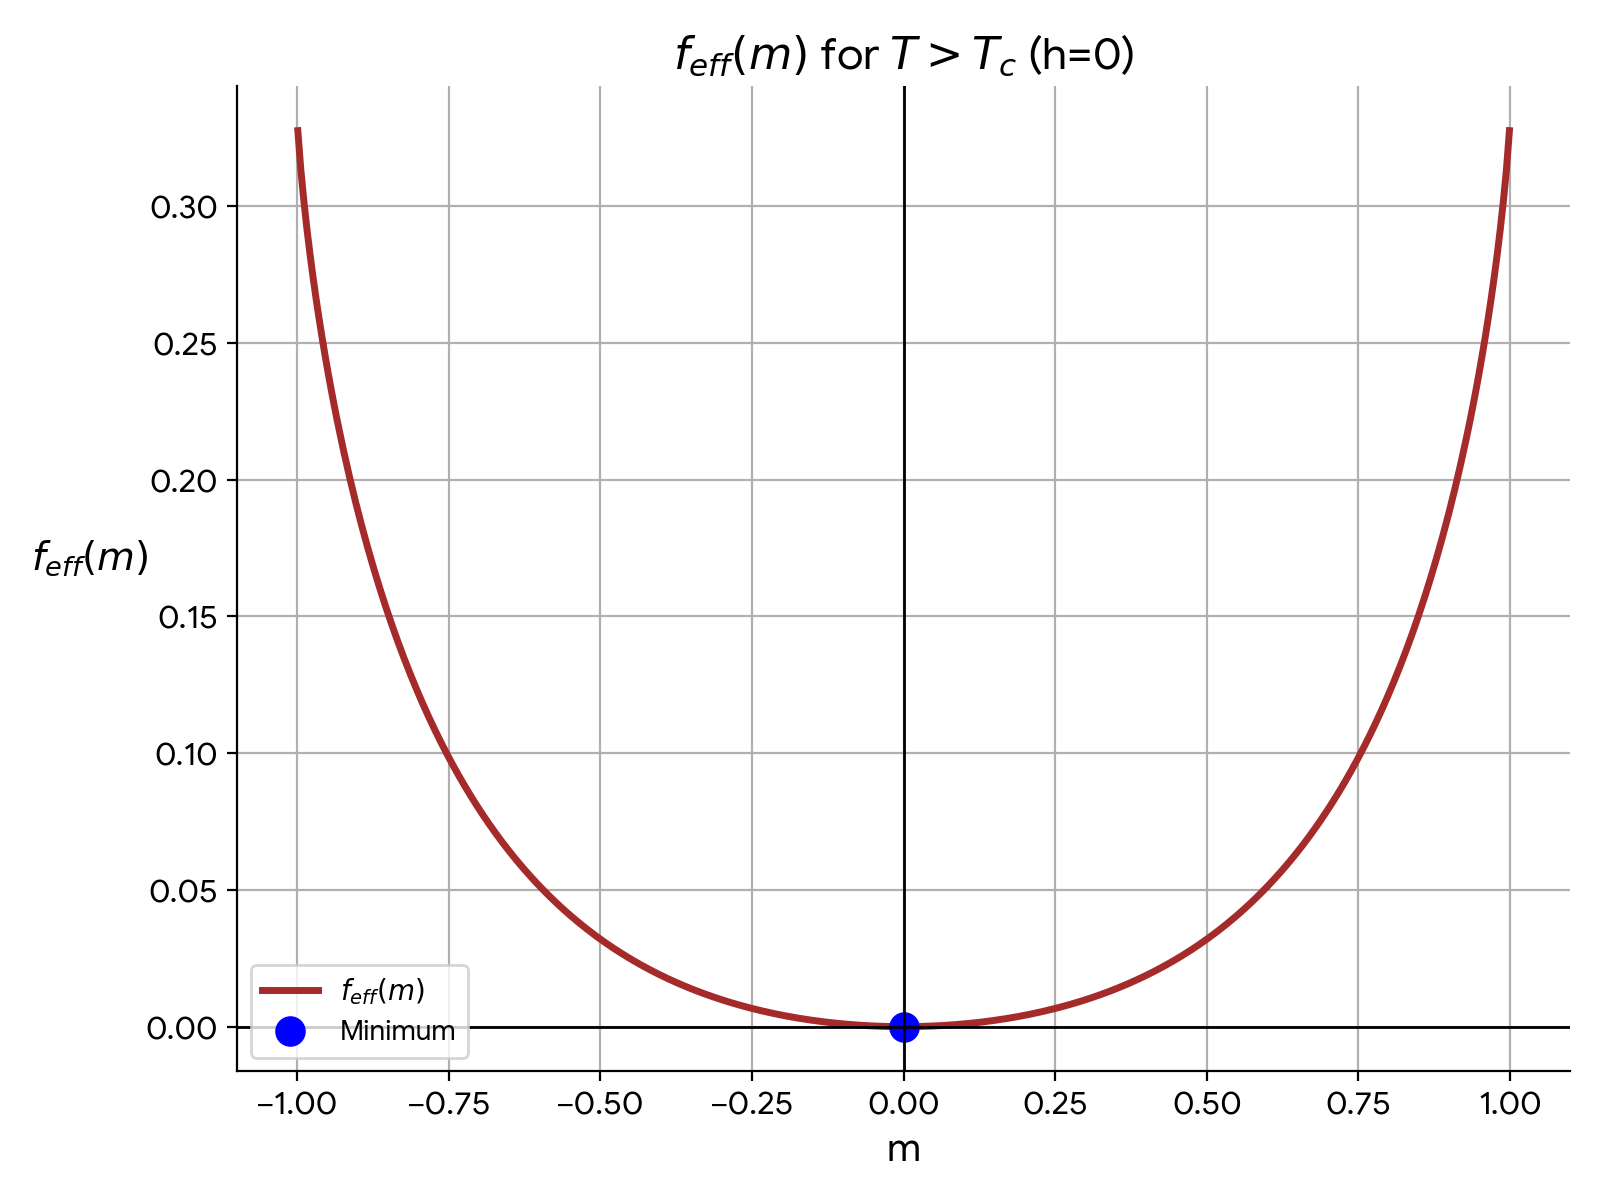
\includegraphics[width=0.6\textwidth]{pics/17_6.png} % INSERIRE QUI IL PERCORSO DEL GRAFICO DELLA DOPPIA BUCA
\caption{Profilo dell'energia libera efficace $f_{eff}(m)$ per $T > T_c$.}
\label{fig:ch17_6}
\end{figure}
    \item \textbf{$T = T_c$}: Il minimo in $m=0$ diventa molto piatto. Sia la derivata prima che la derivata seconda sono zero in $m=0$. Una derivata seconda nulla è associata a una suscettibilità magnetica divergente, $\chi = \frac{dm}{dh}\Big|_{h=0} \to \infty$, che è un segno distintivo di una transizione di fase continua (del secondo ordine).
     \begin{figure}[h!]
\centering
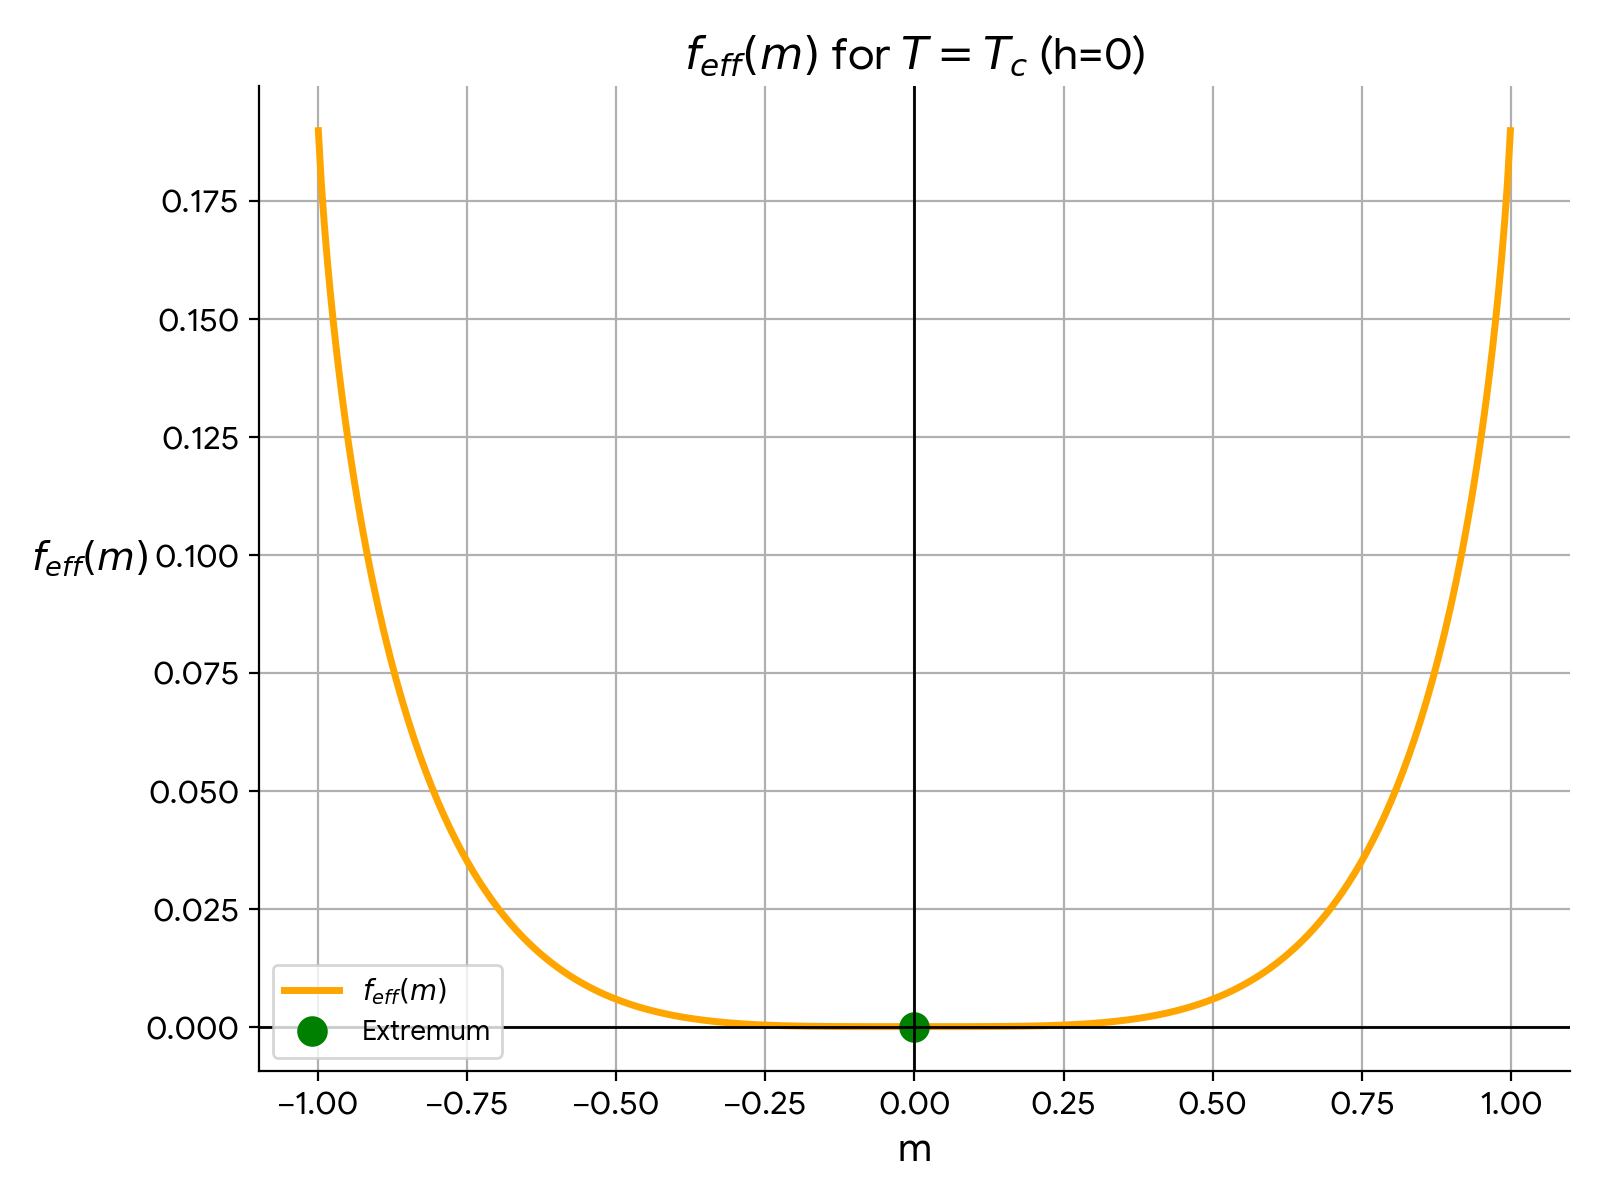
\includegraphics[width=0.6\textwidth]{pics/17_7.png} % INSERIRE QUI IL PERCORSO DEL GRAFICO DELLA DOPPIA BUCA
\caption{Profilo dell'energia libera efficace $f_{eff}(m)$ per $T = T_c$.}
\label{fig:ch17_7}
\end{figure}
    \item \textbf{$T < T_c$}: La forma della funzione cambia in una "doppia buca" (double well). Ci sono due minimi simmetrici in $m^\pm$, che sono le soluzioni stabili. Il punto $m=0$ è ora un massimo locale, che corrisponde a una soluzione instabile.
 \begin{figure}[h!]
\centering
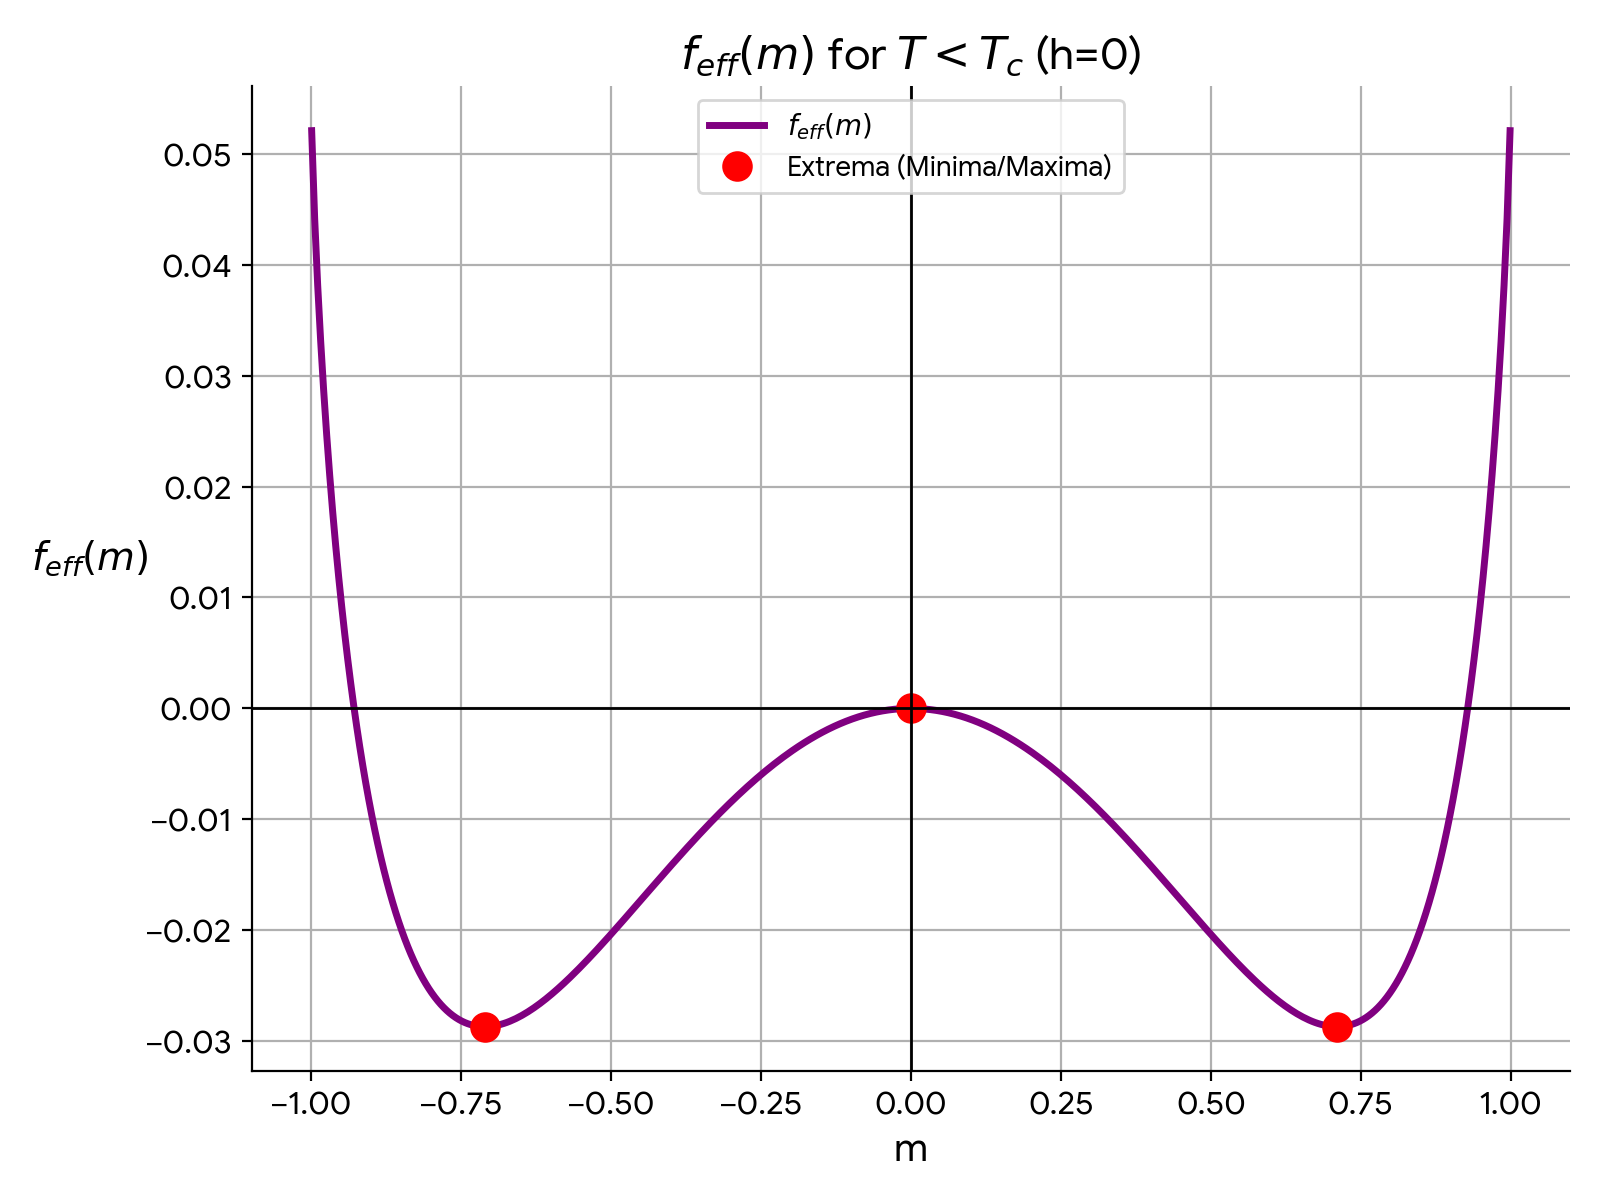
\includegraphics[width=0.6\textwidth]{pics/17_8.png} % INSERIRE QUI IL PERCORSO DEL GRAFICO DELLA DOPPIA BUCA
\caption{Profilo dell'energia libera efficace $f_{eff}(m)$ per $T < T_c$.}
\label{fig:ch17_8}
\end{figure}
\end{itemize}



\subsection*{Caso: $T > T_c$ e $h > 0$}
Consideriamo ora cosa accade quando viene applicato un campo esterno. Esaminiamo il caso ad alta temperatura in presenza di un campo positivo.

Dobbiamo risolvere $m = \tanh(\beta h + \beta z J m)$. La retta $y=m$ non cambia. La curva della tangente iperbolica, invece, è traslata. Il suo argomento si annulla non più in $m=0$, ma quando:

\begin{equation} \label{eq:ch17_23}
\beta h + \beta z J m = 0 \implies m_0 = -\frac{h}{zJ}
\end{equation}

Poiché siamo nel regime $T > T_c$, la pendenza della tangente iperbolica è sempre minore di 1.
Di conseguenza, la curva traslata interseca la retta $y=m$ in un solo punto, che corrisponde a un valore di magnetizzazione $m_{eq} > 0$. La magnetizzazione di equilibrio è sempre positiva se il campo è positivo. Il comportamento qualitativo di $m$ in funzione di $h$ è simile a quello del caso non interagente.

 \begin{figure}[h!]
\centering
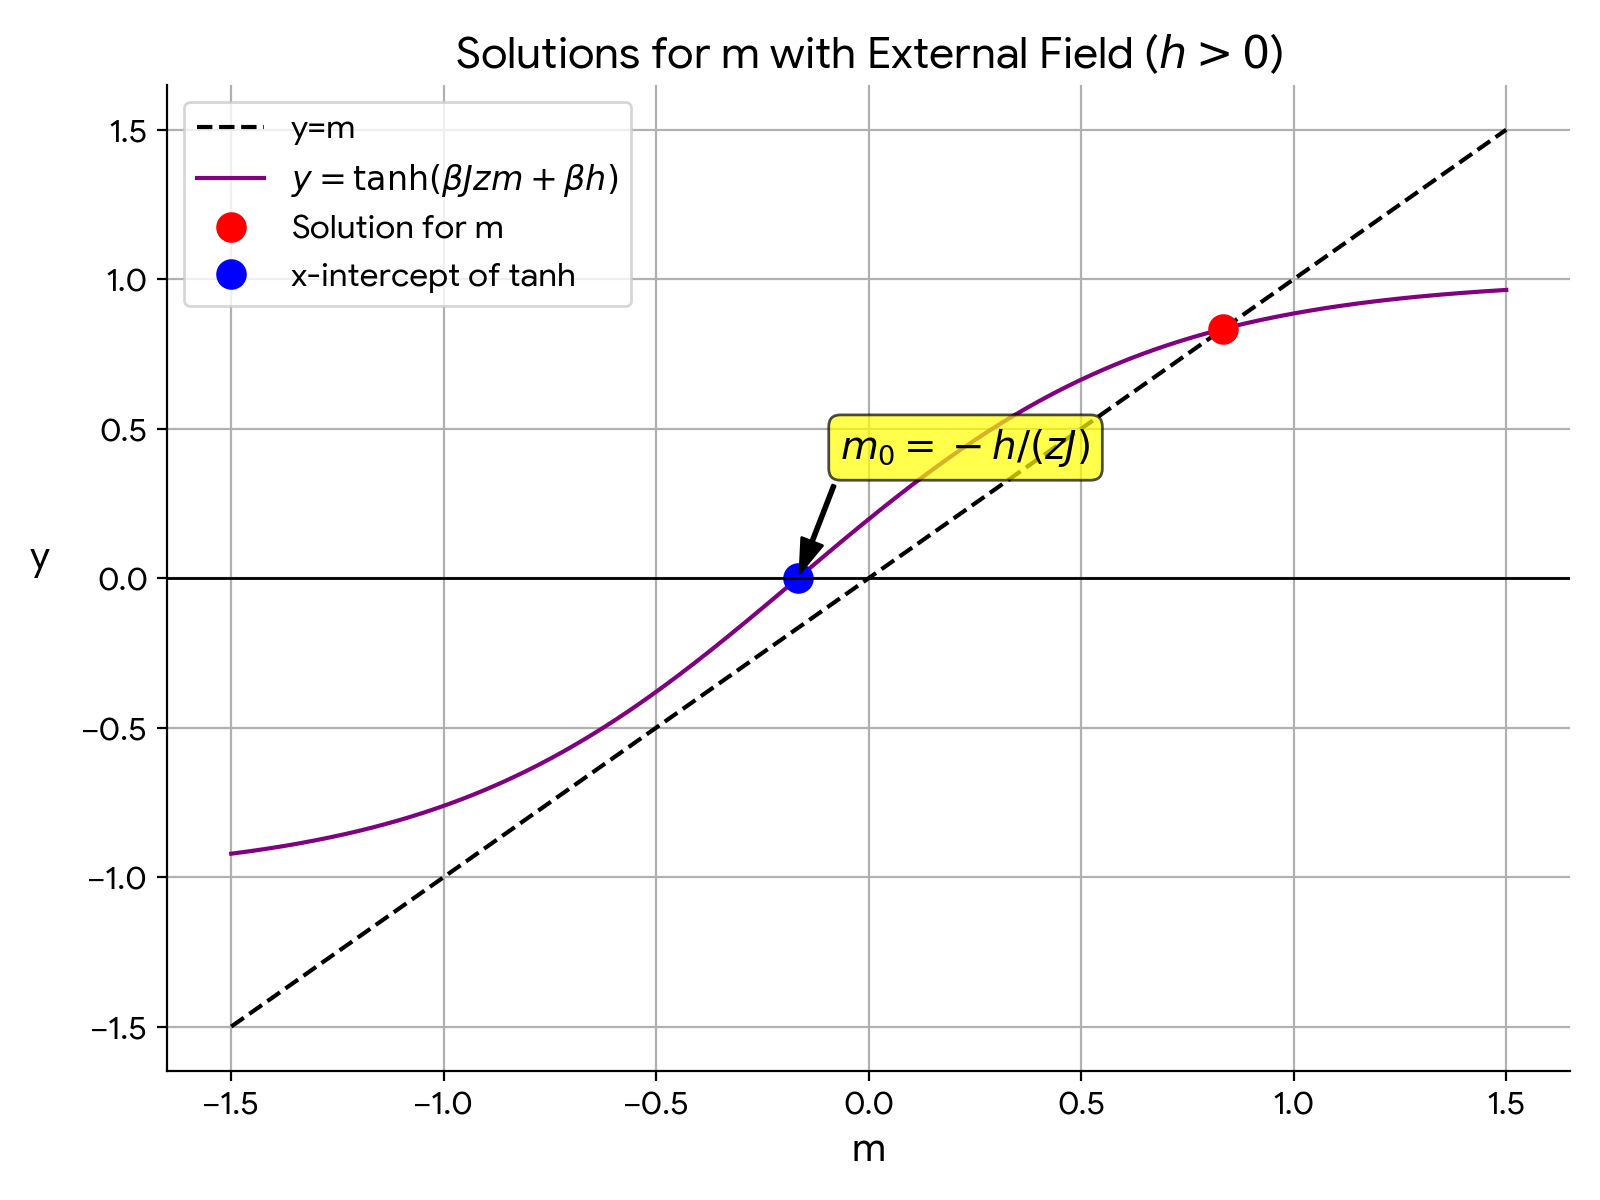
\includegraphics[width=0.6\textwidth]{pics/17_9.png} % INSERIRE QUI IL PERCORSO DEL GRAFICO DELLA DOPPIA BUCA
\caption{Soluzione grafica per $h > 0$.}
\label{fig:ch17_9}
\end{figure}

In questo stesso regime ($T > T_c$, $h>0$), la funzione di energia libera efficace $f_{eff}(m)$ presenta un singolo minimo. A causa del campo esterno, questo minimo non è più in $m=0$, ma è spostato sull'asse positivo, in corrispondenza del valore $m_{eq}$ trovato con il metodo grafico. Questo conferma che c'è un unico stato di equilibrio stabile con magnetizzazione positiva.

\begin{figure}[h!]
\centering
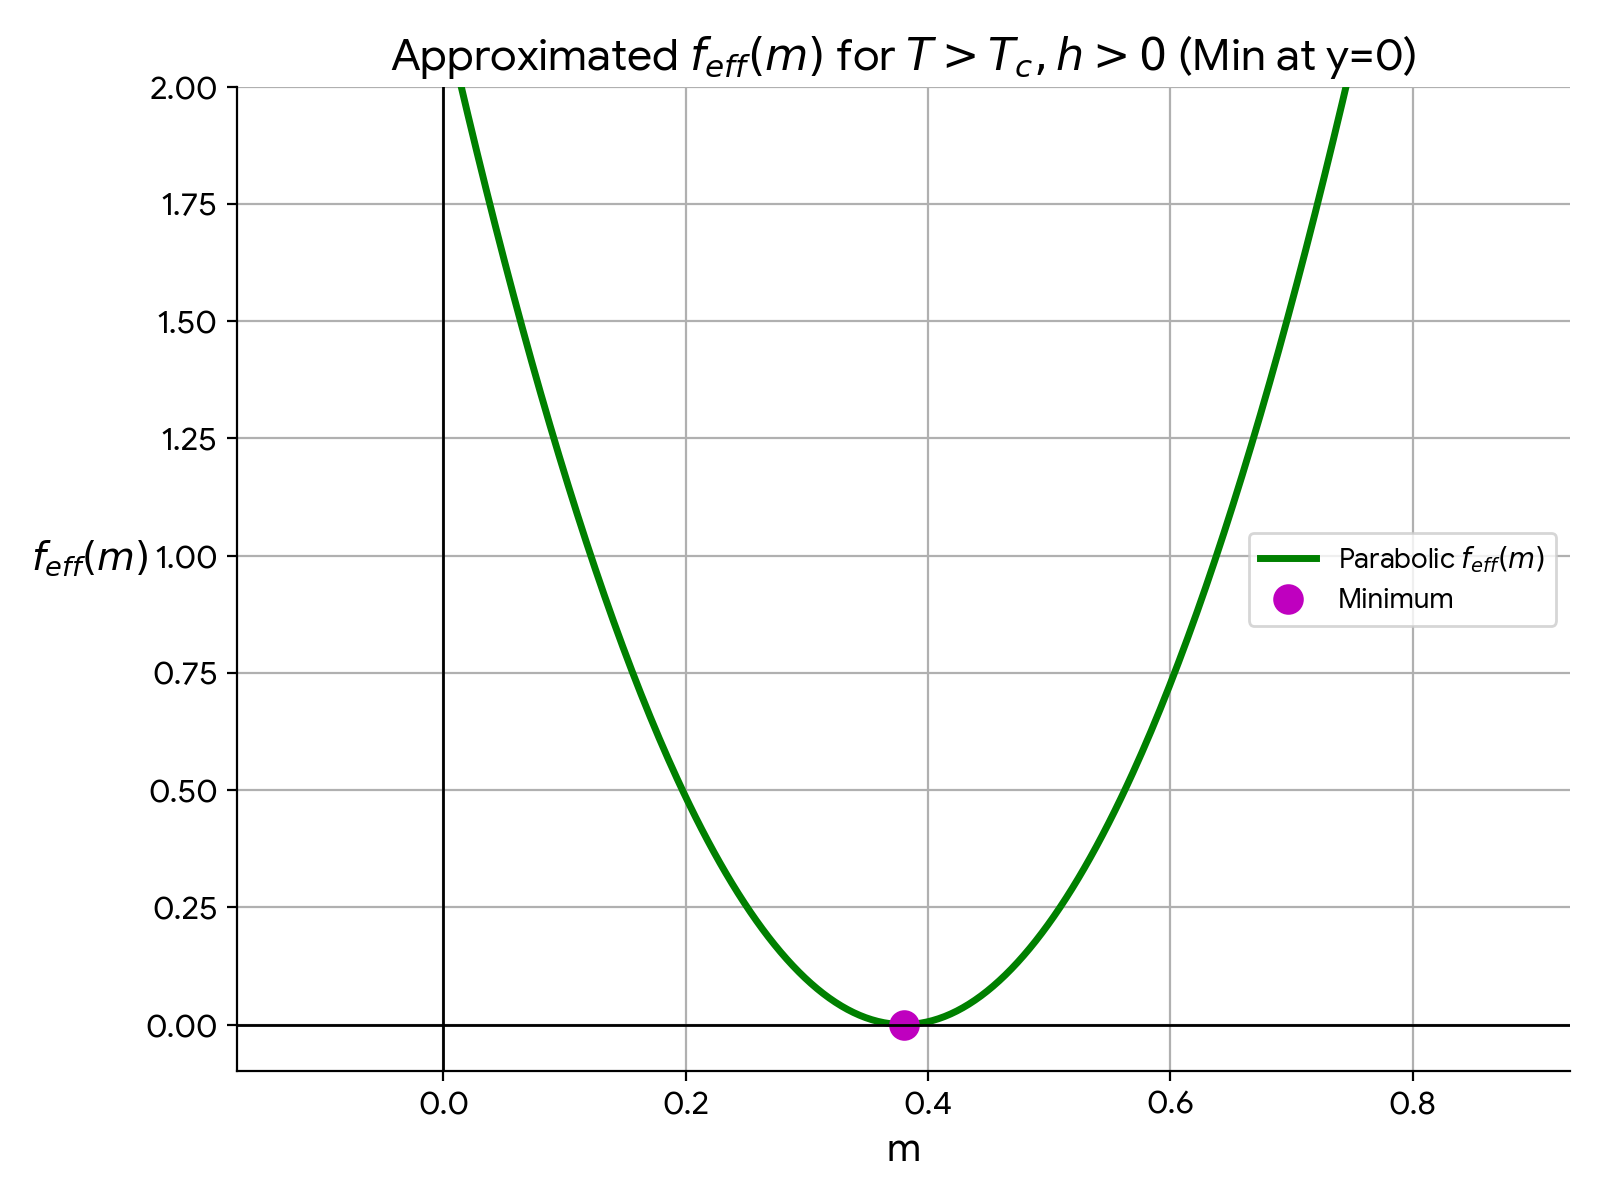
\includegraphics[width=0.6\textwidth]{pics/17_10.png} % INSERIRE QUI IL PERCORSO DEL GRAFICO CON CAMPO ESTERNO
\caption{Energia libera efficace $f_{eff}(m)$ nel caso $T > T_c$ e $h > 0$.}
\label{fig:ch17_10}
\end{figure}




%-------------------------------------------------------------------------------
% CAPITOLO 18
%-------------------------------------------------------------------------------
\chapter{Lezione 18}
\label{capitolo_18}
\textit{08/05/2025}

\section{Isteresi, Transizioni di Fase ed Esponenti Critici}

\subsection*{Comportamento del Sistema per $T < T_c$ con Campo Esterno $h$}
Quando la temperatura del sistema è inferiore alla temperatura critica ($T < T_c$), l'applicazione di un campo magnetico esterno $h$ modifica il comportamento della magnetizzazione $m$.
L'equazione di stato nel modello di campo medio è data da:

\begin{equation} \label{eq:ch18_1}
m = \tanh(\beta h + \beta J z m)
\end{equation}

\begin{itemize}
    \item \textbf{Effetto del Campo:} Se applichiamo un campo $h > 0$, l'intera curva $\tanh(x)$ viene traslata verso sinistra, mentre il potenziale efficace $f_{eff}(m)$ viene spinto verso destra.
Man mano che $h$ diminuisce, la curva $\tanh(x)$ si sposta verso destra e $m_{eq}$ si sposta verso sinistra.
    \item \textbf{Effetto della Temperatura:} Se diminuiamo la temperatura $T$, la pendenza della funzione $\tanh(x)$ nell'origine diventa più ripida. Questo favorisce un maggiore ordine e quindi una magnetizzazione più grande.
\end{itemize}

A una certa temperatura, definita Temperatura Spinodale, la comparsa di una seconda intersezione tra la retta $y=m$ e la curva $\tanh$ segnala la formazione di un secondo minimo nel potenziale efficace $f_{eff}(m)$.
Questo nuovo minimo è metastabile: ha un'energia libera più alta del minimo globale (lo stato di equilibrio vero) ma è comunque un punto di equilibrio localmente stabile. Per $h > 0$, lo stato con magnetizzazione positiva è favorito, quindi il suo minimo di energia libera sarà più basso.

Un comportamento simile si osserva mantenendo $T < T_c$ fissa e riducendo il campo $h$ da un valore elevato. Esiste un campo spinodale al di sotto del quale compare lo stato metastabile.

Per tempi di osservazione finiti, il sistema può rimanere "intrappolato" in questo stato metastabile.


\section{Isteresi e Transizione di Fase del 1° Ordine}
Il fenomeno dell'isteresi emerge quando si traccia la magnetizzazione $m$ in funzione del campo $h$ a temperatura costante $T < T_c$.

\begin{itemize}
    \item \textbf{Ramo di Equilibrio:} Partendo da $h \gg 0$, il sistema si trova nel suo stato di equilibrio con $m > 0$. Riducendo lentamente $h$, il sistema segue il ramo di equilibrio della curva.
    \item \textbf{Ramo Metastabile:} Se il campo viene ridotto e poi invertito ($h < 0$) rapidamente, il sistema può persistere nello stato con $m > 0$, che ora è metastabile. Questo ramo è una continuazione del ramo di equilibrio.
    \item \textbf{Transizione Discontinua:} Per un valore di $h$ sufficientemente negativo, lo stato metastabile scompare e il sistema "salta" bruscamente allo stato di equilibrio con magnetizzazione negativa.
\end{itemize}

Questo ciclo $m(h)$ è noto come ciclo di isteresi. Il salto della magnetizzazione a $h = 0$ (in condizioni sperimentali standard) è una transizione di fase discontinua del primo ordine.
Viene definita del primo ordine perché la grandezza che presenta una discontinuità, il parametro d'ordine $m$, è la derivata prima dell'energia libera $F$ rispetto al campo $h$.

\vspace{0.5cm}
\noindent\fbox{%
    \parbox{\dimexpr\linewidth-2\fboxsep-2\fboxrule\relax}{%
        \begin{equation} \label{eq:ch18_2}
        m = -\frac{1}{N}\frac{\partial F}{\partial h}
        \end{equation}
    }%
}
\vspace{0.5cm}

La prova di questa relazione è la seguente:

\begin{equation} \label{eq:ch18_3}
F(T, N, h) = -\frac{1}{\beta} \ln(Z)
\end{equation}

\begin{equation} \label{eq:ch18_4}
Z = \sum_{\{S_i\}} e^{-\beta H(\{S_i\})} \quad \text{con} \quad H = -J\sum_{\langle i,j \rangle} S_i S_j - h\sum_i S_i
\end{equation}

Calcoliamo la derivata:

\begin{equation} \label{eq:ch18_5}
-\frac{1}{N}\frac{\partial F}{\partial h} = -\frac{1}{N} \frac{\partial}{\partial h} \left( -\frac{1}{\beta} \ln Z \right) = \frac{1}{N\beta} \frac{1}{Z} \frac{\partial Z}{\partial h}
\end{equation}

\begin{equation} \label{eq:ch18_6}
\frac{\partial Z}{\partial h} = \frac{\partial}{\partial h} \sum_{\{S_i\}} e^{-\beta H} = \sum_{\{S_i\}} e^{-\beta H} \left( -\beta \frac{\partial H}{\partial h} \right) = \sum_{\{S_i\}} e^{-\beta H} \left( \beta \sum_i S_i \right)
\end{equation}

Sostituendo, otteniamo:

\begin{equation} \label{eq:ch18_7}
-\frac{1}{N}\frac{\partial F}{\partial h} = \frac{1}{N\beta} \frac{1}{Z} \sum_{\{S_i\}} \left(\beta \sum_i S_i\right) e^{-\beta H} = \frac{1}{N} \sum_i \left( \sum_{\{S_i\}} S_i \frac{e^{-\beta H}}{Z} \right) = \frac{1}{N} \sum_i \langle S_i \rangle = m
\end{equation}

Poiché $m$ (la derivata prima di $F$) ha un salto, la transizione è del primo ordine e discontinua.


\section{Transizione di Fase del 2° Ordine ed Esponenti Critici}
Se fissiamo $h=0$ e variamo la temperatura $T$, osserviamo una transizione di fase del secondo ordine a $T = T_c$. È detta continua perché $m$ va a zero con continuità. L'anomalia si trova nella derivata seconda dell'energia libera.
La suscettibilità magnetica $\chi$ è la derivata seconda di $F$:

\vspace{0.5cm}
\noindent\fbox{%
    \parbox{\dimexpr\linewidth-2\fboxsep-2\fboxrule\relax}{%
        \begin{equation} \label{eq:ch18_8}
        \chi := \frac{\partial m}{\partial h}\bigg|_{h=0} = -\frac{1}{N}\frac{\partial^2 F}{\partial h^2}\bigg|_{h=0}
        \end{equation}
    }%
}
\vspace{0.5cm}

Per $T$ vicino a $T_c$ e $h$ piccolo, linearizziamo l'equazione di campo medio: $m \approx \beta h + \beta z J m$.
Da cui:

\begin{equation} \label{eq:ch18_9}
(1 - \beta z J)m \approx \beta h \implies \chi = \frac{m}{h} = \frac{\beta}{1 - \beta z J}
\end{equation}

Ricordando che $T_c = zJ/k_B$, si può riscrivere il denominatore come $1 - T_c/T = (T - T_c)/T$

\begin{equation} \label{eq:ch18_10}
\chi \propto \frac{1}{T - T_c}
\end{equation}

Quindi $\chi$ diverge per $T \to T_c$.

\subsection*{Calcolo degli Esponenti Critici}
Gli esponenti critici descrivono il comportamento delle grandezze fisiche vicino al punto critico.

\begin{itemize}
    \item \textbf{Esponente $\gamma$ (Suscettibilità):} Definito da $\chi \sim (T - T_c)^{-\gamma}$. Il nostro calcolo mostra $\gamma = 1$ in campo medio.
    \item \textbf{Esponente $\beta$ (Parametro d’ordine):} Definito da $m \sim (T_c - T)^{\beta}$ per $T < T_c$ e $h=0$. Sviluppiamo $\tanh(x) \approx x - x^3/3$:
\end{itemize}

\begin{equation} \label{eq:ch18_11}
m = \tanh(\beta z J m) \approx (\beta z J m) - \frac{1}{3}(\beta z J m)^3
\end{equation}

Semplificando $m$ e riarrangiando:

\begin{equation} \label{eq:ch18_12}
1 \approx \beta z J - \frac{1}{3}(\beta z J)^3 m^2 \implies m^2 \approx \frac{3( \beta z J - 1)}{(\beta z J)^3} = \frac{3(T_c/T - 1)}{(T_c/T)^3}
\end{equation}

Per $T \approx T_c$, $m^2 \propto (T_c - T)$, quindi $\beta = 1/2$ in campo medio.

\begin{itemize}
    \item \textbf{Esponente $\delta$ (Isoterma Critica):} Definito da $m \sim h^{1/\delta}$ a $T = T_c$. A $T_c$, si ha $\beta_c z J = 1$
\end{itemize}

L'espansione diventa:

\begin{equation*} 
m = \tanh(\beta_c h + \beta_c z J m) = \tanh(\beta_c h + m) \approx (\beta_c h + m) - \frac{1}{3}(\beta_c h + m)^3
\end{equation*}

Trascurando $m$ a primo ordine, si ottiene:

\begin{equation} \label{eq:ch18_13}
0 \approx \beta_c h - \frac{1}{3}(\beta_c h + m)^3
\end{equation}

Per $h$ piccolo, $m$ domina nel termine cubico: $m^3 \approx 3 \beta_c h$, da cui $m \sim h^{1/3}$.
Quindi $\delta = 3$ in campo medio.

Sistemi fisici molto diversi possono condividere gli stessi esponenti critici, appartenendo così alla stessa classe di universalità. Questo implica che il comportamento collettivo su larga scala vicino a una transizione di fase è indipendente dai dettagli microscopici del sistema. Questo concetto permette di usare modelli semplici per predire il comportamento di sistemi complessi.


\section{Funzioni di Correlazione e FDT}
Per analizzare il comportamento collettivo, si usa la funzione di correlazione connessa:

\begin{equation} \label{eq:ch18_14}
C_{ij}^{conn} = \langle S_i S_j \rangle - \langle S_i \rangle \langle S_j \rangle
\end{equation}

Questa funzione è non nulla solo se il sistema è interagente. Poiché l'approssimazione di campo medio tratta gli spin come indipendenti, darebbe erroneamente $C_{ij}^{conn} = 0$. Si aggira il problema usando il Teorema di Fluttuazione-Dissipazione (FDT), che lega la correlazione alla risposta del sistema a una perturbazione:

\vspace{0.5cm}
\noindent\fbox{%
    \parbox{\dimexpr\linewidth-2\fboxsep-2\fboxrule\relax}{%
        \begin{equation} \label{eq:ch18_15}
        \chi_{ij} = \frac{\partial \langle S_i \rangle}{\partial h_j} \bigg|_{h=0}= \beta C_{ij}^{conn} \bigg|_{h=0}
        \end{equation}
    }%
}
\vspace{0.5cm}

\textbf{Dimostrazione del FDT:}

Partiamo da $\langle S_i \rangle = (1/Z) \sum_{\{S_k\}} S_i e^{-\beta H}$. Derivando rispetto a $h_j$:

\begin{equation} \label{eq:ch18_16}
\frac{\partial \langle S_i \rangle}{\partial h_j} = \frac{\partial}{\partial h_j} \left( \frac{1}{Z} \right) \sum S_i e^{-\beta H} + \frac{1}{Z} \sum S_i \frac{\partial}{\partial h_j} (e^{-\beta H})
\end{equation}

Usando $\partial(e^{-\beta H})/\partial h_j = \beta S_j e^{-\beta H}$ e $\partial(1/Z)/\partial h_j = -(1/Z^2) \partial Z/\partial h_j = -(1/Z) \beta \langle S_j \rangle$, si ottiene:

\begin{equation} \label{eq:ch18_17}
\frac{\partial \langle S_i \rangle}{\partial h_j} = -\beta \langle S_j \rangle \langle S_i \rangle + \beta \langle S_i S_j \rangle
\end{equation}

Che, per $h=0$, è esattamente l'FDT:

\begin{equation} \label{eq:ch18_18}
\chi_{ij}\bigg|_{h=0} = \beta [ \langle S_i S_j \rangle - \langle S_i \rangle \langle S_j \rangle ]\bigg|_{h=0}
\end{equation}

Questo teorema è cruciale: lega le fluttuazioni interne del sistema a riposo ($C_{ij}^{conn}$) alla sua risposta lineare a una perturbazione esterna ($\chi_{ij}$).

%-------------------------------------------------------------------------------
% CAPITOLO 19
%-------------------------------------------------------------------------------
\chapter{Lezione 19}
\label{capitolo_19}

\section{Funzione di Correlazione}
Iniziamo definendo la funzione di correlazione connessa $C_{ij}^c$ tra due spin $S_i$ e $S_j$ situati nei siti $i$ e $j$ di un reticolo:

\begin{equation} \label{eq:ch19_1}
C_{ij}^{c} = \langle S_i S_j \rangle - \langle S_i \rangle \langle S_j \rangle
\end{equation}

Nell'approssimazione di campo medio, che considera il miglior modello non interattivo per approssimare il nostro modello fortemente interattivo, le funzioni di correlazione risultano essere zero. Questo avviene perché, intrinsecamente, tale approssimazione annulla le correlazioni, anche se nel sistema reale (senza approssimazione) esse non sono nulle.
Per calcolare comunque queste funzioni di correlazione nel contesto in cui stiamo lavorando, possiamo sfruttare il Teorema Fluttuazione-Dissipazione (FDT). Questo teorema mette in relazione la funzione di correlazione magnetica con la suscettibilità del sistema. La relazione è la seguente:

\begin{equation} \label{eq:ch19_2}
\chi_{ij} = \beta C_{ij}^{c}
\end{equation}

dove $\chi_{ij}$ è la matrice di suscettibilità, definita come la funzione di risposta che descrive la risposta lineare del sistema all'applicazione di un campo esterno $h_j$:

\begin{equation} \label{eq:ch19_3}
\chi_{ij} = \frac{\partial \langle S_i \rangle}{\partial h_j} \bigg|_{h=0}
\end{equation}

Possiamo calcolare la funzione di suscettibilità nell'approssimazione di campo medio. Quindi, attraverso la FDT, otteniamo in modo indiretto la funzione di correlazione stessa.


\section{Invarianza Traslazionale e Spazio di Fourier}
Le funzioni $C_{ij}$ e $\chi_{ij}$ dipendono dalle posizioni spaziali dei siti $i$ e $j$, che indichiamo con $\bar{r}_i$ e $\bar{r}_j$.
Consideriamo un sistema definito su un reticolo regolare, ad esempio un reticolo 2D dove ogni spin $S_i$ è localizzato in una specifica posizione $\bar{r}_i$.
In assenza di un campo magnetico esterno, il sistema è perfettamente invariante per traslazioni spaziali. Di conseguenza, una funzione che in principio dipende da due coordinate $\bar{r}_i$ e $\bar{r}_j$, come $C^c(\bar{r}_i, \bar{r}_j)$, dipenderà in realtà solo dalla loro distanza relativa $\bar{r}_{ij} = \bar{r}_i - \bar{r}_j$:

\begin{equation} \label{eq:ch19_4}
C^c(\bar{r}_i, \bar{r}_j) \rightarrow C^c(\bar{r}_{ij})
\end{equation}

Lo stesso vale per la suscettibilità:

\begin{equation} \label{eq:ch19_5}
\chi(\bar{r}_i, \bar{r}_j) \rightarrow \chi(\bar{r}_{ij})
\end{equation}

Questo significa che il comportamento fisico tra due punti $i$ e $j$ non dipende specificamente dalla loro posizione assoluta nel reticolo, ma solo dalla loro distanza relativa (assumendo condizioni al contorno periodiche o di essere lontani dai bordi).
Se il modello possiede anche invarianza rotazionale (isotropia), allora la dipendenza sarà solo dal modulo della distanza, $r_{ij} = |\bar{r}_{ij}|$.
L'invarianza traslazionale rende conveniente lavorare nello spazio di Fourier. La trasformata di Fourier di una funzione dipendente solo da $\bar{r}_{ij}$ dipenderà da un solo vettore d'onda $\bar{q}$.
Per la funzione di correlazione connessa e la suscettibilità avremo:

\begin{equation} \label{eq:ch19_6}
C^c(\bar{r}_{ij}) \xrightarrow{\text{Fourier T.}} \hat{C}^c(\bar{q})
\end{equation}

\begin{equation} \label{eq:ch19_7}
\chi(\bar{r}_{ij}) \xrightarrow{\text{Fourier T.}} \hat{\chi}(\bar{q}) = \frac{\partial \hat{m}(\bar{q})}{\partial \hat{h}(\bar{q})}
\end{equation}

dove $\hat{m}(\bar{q})$ e $\hat{h}(\bar{q})$ sono le trasformate di Fourier della magnetizzazione e del campo magnetico, rispettivamente. La strategia consiste nel calcolare $\hat{\chi}(\bar{q})$, da cui si ottiene $\hat{C}^c(\bar{q})$ tramite la FDT, e infine antitrasformando per ottenere $C^c(\bar{r}_{ij})$.
Il punto di partenza è l'equazione di campo medio per la magnetizzazione $m_i$ sul sito $i$. Nel caso di un campo omogeneo $h$, tutte le magnetizzazioni locali $m_i$ sono uguali alla magnetizzazione globale $m$, e l'equazione è:

\begin{equation} \label{eq:ch19_8}
m = \tanh(\beta h + \beta J z m)
\end{equation}

dove $z$ è il numero di primi vicini e $J$ è la costante di accoppiamento.
Per calcolare la suscettibilità $\chi_{ij}$, che descrive la risposta a un campo locale $h_j$, dobbiamo generalizzare l'equazione di campo medio al caso in cui il campo $h_i$ può variare da sito a sito (campo disomogeneo). In questo caso, anche la magnetizzazione media locale $m_i = \langle S_i \rangle$ varierà da sito a sito. L'equazione generalizzata diventa:

\vspace{0.5cm}
\noindent\fbox{%
    \parbox{\dimexpr\linewidth-2\fboxsep-2\fboxrule\relax}{%
        \begin{equation} \label{eq:ch19_9}
        m_i = \tanh\left(\beta h_i + \beta J \sum_{l \in N_i} m_l\right)
        \end{equation}
    }%
}
\vspace{0.5cm}

dove $N_i$ indica l'insieme dei primi vicini del sito $i$.
Risolvere questo sistema di $N$ equazioni accoppiate per $m_i$ nello spazio reale è complicato perché non è direttamente invertibile. Per questo motivo, passiamo allo spazio di Fourier, dove le equazioni si disaccoppiano e diventano invertibili.


\section{Linearizzazione e Trasformata di Fourier}
Vogliamo studiare il comportamento della suscettibilità e della funzione di correlazione vicino alla temperatura critica $T_c$, approcciandola dalla fase ad alta temperatura ($T \rightarrow T_c^+$). In questa regione, la magnetizzazione è zero in assenza di campo.
Se applichiamo un campo $h_i$ molto piccolo, anche la risposta $m_i$ sarà piccola. Possiamo quindi espandere la tangente iperbolica al primo ordine ($\tanh(x) \approx x$ per $x \ll 1$). L'equazione linearizzata diventa:

\begin{equation} \label{eq:ch19_10}
m_i \approx \beta h_i + \beta J \sum_{l \in N_i} m_l
\end{equation}

Definiamo la trasformata di Fourier discreta e la sua inversa come segue:

\begin{equation} \label{eq:ch19_11}
\hat{m}_{\bar{q}} = \sum_{\bar{r}_i} e^{-i\bar{q}\cdot\bar{r}_i} m_i
\end{equation}

\begin{equation} \label{eq:ch19_12}
m_i = \frac{1}{N} \sum_{\bar{q}} e^{i\bar{q}\cdot\bar{r}_i} \hat{m}_{\bar{q}}
\end{equation}

La posizione del fattore $1/N$ è convenzionale.
Applichiamo la trasformata di Fourier all'equazione linearizzata:
\begin{itemize}
    \item Il membro sinistro $m_i$ diventa $\hat{m}_{\bar{q}}$
    \item Il termine $\beta h_i$ diventa $\beta \hat{h}_{\bar{q}}$
\end{itemize}

Per il termine di interazione, dobbiamo essere più attenti:

\begin{equation} \label{eq:ch19_13}
\text{TF}\left[\beta J \sum_{j \in N_i} m_j\right] = \sum_{\bar{r}_i} e^{-i\bar{q}\cdot\bar{r}_i} \beta J \sum_{l \in N_i} \left(\frac{1}{N} \sum_{\bar{k}} e^{i\bar{k}\cdot\bar{r}_l} \hat{m}_{\bar{k}}\right)
\end{equation}

Ponendo $\bar{r}_l = \bar{r}_i + \bar{r}_{il}$:

\begin{equation} \label{eq:ch19_14}
\frac{\beta J}{N} \sum_{\bar{r}_i} e^{-i\bar{q}\cdot\bar{r}_i} \sum_{l \in N_i} \sum_{\bar{k}} e^{i\bar{k}\cdot(\bar{r}_i + \bar{r}_{il})} \hat{m}_{\bar{k}}
\end{equation}

Raggruppiamo i termini che dipendono da $\bar{r}_i$:

\begin{equation} \label{eq:ch19_15}
\frac{\beta J}{N} \sum_{\bar{k}} \sum_{\bar{r}_i} e^{-i\bar{r}_i \cdot (\bar{q}-\bar{k})} \left( \sum_{l \in N_i} e^{i\bar{k}\cdot\bar{r}_{il}} \right) \hat{m}_{\bar{k}}
\end{equation}

La somma $\frac{1}{N}\sum_{\bar{r}_i} e^{-i(\bar{q}-\bar{k})\cdot\bar{r}_i}$ è una rappresentazione della delta di Kronecker $\delta(\bar{q}-\bar{k})$, quindi:

\begin{equation} \label{eq:ch19_16}
\beta J \sum_{\bar{k}} \delta(\bar{q}-\bar{k}) \left( \sum_{l \in N_i} e^{i\bar{k}\cdot\bar{r}_{il}} \right) \hat{m}_{\bar{k}}
\end{equation}

La presenza della $\delta$ nella somma su $\bar{k}$ significa che solo il termine con $\bar{k}=\bar{q}$ sopravvive:

\begin{equation} \label{eq:ch19_17}
\beta J  \left( \sum_{l \in N_i} e^{i\bar{q}\cdot\bar{r}_{il}} \right) \hat{m}_{\bar{q}}
\end{equation}

La somma $\sum_{l \in N_i} e^{i\bar{q}\cdot\bar{r}_{il}}$ è una somma sui vettori che connettono il sito $i$ ai suoi primi vicini. Per un reticolo regolare, questa somma ha lo stesso valore per ogni sito $i$ e non dipende da $\bar{r}_i$.
Per un reticolo ipercubico $d$-dimensionale con passo reticolare $L$, i vettori $\bar{r}_{il}$ che connettono ai primi vicini sono $(\pm L, 0, \dots)$, $(0, \pm L, \dots)$, ecc. La somma diventa:

\begin{equation} \label{eq:ch19_18}
\sum_{l \in N_i} e^{i\bar{q}\cdot\bar{r}_{il}} = \sum_{\alpha=1}^{d} (e^{iq_{\alpha}L} + e^{-iq_{\alpha}L}) = \sum_{\alpha=1}^{d} 2\cos(q_{\alpha}L)
\end{equation}

L'equazione trasformata completa è quindi:

\begin{equation} \label{eq:ch19_19}
\hat{m}_{\bar{q}} = \beta \hat{h}_{\bar{q}} + \beta J \hat{m}_{\bar{q}} \sum_{\alpha=1}^{d} 2\cos(q_{\alpha}L)
\end{equation}

Risolvendo per $\hat{m}_{\bar{q}}$:

\begin{equation} \label{eq:ch19_20}
\hat{m}_{\bar{q}} = \frac{\beta \hat{h}_{\bar{q}}}{1 - 2\beta J \sum_{\alpha=1}^{d} \cos(q_{\alpha}L)}
\end{equation}

Dalla definizione $\hat{\chi}(\bar{q}) =\frac{\partial \hat{m}_{\bar{q}} }{ \partial \hat{h}_{\bar{q}}}$, e usando $\hat{C}^c(\bar{q}) = \frac{1}{\beta} \hat{\chi}(\bar{q})$, otteniamo:

\begin{equation} \label{eq:ch19_21}
\hat{C}^c(\bar{q}) = \frac{1}{1 - 2\beta J \sum_{\alpha=1}^{d} \cos(q_{\alpha}L)}
\end{equation}

Siamo interessati al comportamento della funzione di correlazione a grandi distanze nello spazio reale: $r \gg L$. Questo corrisponde a piccoli vettori d'onda nello spazio di Fourier: $qL \ll 1$.
In questo limite, possiamo espandere il coseno: $\cos(x) \approx 1 - x^2/2$
Il denominatore di $\hat{C}^c(\bar{q})$ diventa:

\begin{align*}
1 - 2\beta J \sum_{\alpha=1}^{d} \cos(q_{\alpha}L) &\approx 1 - 2\beta J \sum_{\alpha=1}^{d} \left(1 - \frac{(q_{\alpha}L)^2}{2}\right) \\
&= 1 - 2\beta J d + \beta J L^2 \sum_{\alpha=1}^{d} q_{\alpha}^2 \\
&= 1 - \beta J z + \beta J L^2 q^2
\end{align*}

dove $z = 2d$ è il numero di coordinazione per un reticolo ipercubico e $q^2 = \sum_{\alpha} q_{\alpha}^2$ è il modulo quadro del vettore d'onda.
Quindi, per $q \ll 1/L$:

\begin{equation} \label{eq:ch19_22}
\hat{C}^c(\bar{q}) \approx \frac{1}{1 - \beta J z + \beta J L^2 q^2} = \frac{1}{\beta J L^2} \frac{1}{q^2 + \frac{1-\beta J z}{\beta J L^2}}
\end{equation}

Definiamo la lunghezza di correlazione $\xi$ come:

\vspace{0.5cm}
\noindent\fbox{%
    \parbox{\dimexpr\linewidth-2\fboxsep-2\fboxrule\relax}{%
        \begin{equation} \label{eq:ch19_23}
        \xi^{-2} = \frac{1 - \beta J z}{\beta J L^2}
        \end{equation}
    }%
}
\vspace{0.5cm}

Con questa definizione, $\hat{C}^c(\bar{q})$ assume la forma Ornstein-Zernike:

\vspace{0.5cm}
\noindent\fbox{%
    \parbox{\dimexpr\linewidth-2\fboxsep-2\fboxrule\relax}{%
        \begin{equation} \label{eq:ch19_24}
        \hat{C}^c(\bar{q}) = \frac{1}{\beta J L^2} \frac{1}{q^2 + \xi^{-2}}
        \end{equation}
    }%
}
\vspace{0.5cm}

La lunghezza di correlazione $\xi$ ha le dimensioni di una lunghezza. Ricordando che la temperatura critica di campo medio è $T_c = Jz/k_B$, ovvero $\beta_c J z = 1$, possiamo riscrivere $\xi$ come:

\begin{equation} \label{eq:ch19_25}
\xi = \sqrt{\frac{\beta J L^2}{1 - \beta J z}} = \frac{L \sqrt{\beta J}}{\sqrt{1 - \frac{T_c}{T}}}
\end{equation}


\section{Funzione di Correlazione nello Spazio Reale}
Per ottenere la funzione di correlazione nello spazio reale $C^c(\bar{r})$, dobbiamo antitrasformare.
Poiché siamo interessati a grandi distanze, possiamo passare a una trasformata di Fourier continua:

\begin{equation} \label{eq:ch19_26}
C^c(\bar{r}) = \int \frac{d^d q}{(2\pi)^d} e^{i\bar{q}\cdot\bar{r}} \hat{C}^c(\bar{q}) \approx A' \int d^d q \frac{e^{i\bar{q}\cdot\bar{r}}}{q^2 + \xi^{-2}}
\end{equation}

dove $A'$ è una costante.
Consideriamo il caso tridimensionale ($d=3$). L'integrale si calcola passando in coordinate sferiche per $\bar{q}$:

\begin{align} \label{eq:ch19_27}
C^c(\bar{r}) &= A \int_{-1}^{1} d(\cos\theta) \int_0^\infty dq \, q^2 \frac{e^{iqr\cos\theta}}{q^2 + \xi^{-2}} \nonumber \\ 
&=  A \int_0^\infty dq \, q^2 \frac{1}{iqr} \frac{[e^{iqr} - e^{-iqr}]}{q^2 + \xi^{-2}}  \nonumber \\ 
&= \frac{A}{ir} \int_0^\infty dq \frac{q}{q^2 + \xi^{-2}} [e^{iqr} - e^{-iqr}]
\end{align}

L'integrale da $0$ a $\infty$ viene esteso da $-\infty$ a $\infty$ (l'integrando completo è pari, quindi si introduce un fattore $1/2$ assorbito in $A$).
Si considera solo uno dei due termini esponenziali, $e^{iqr}$, poiché il calcolo per $e^{-iqr}$ è analogo e darà un contributo con segno opposto che si sommerà costruttivamente.

\begin{equation*}
\frac{A}{ir} \int_{-\infty}^\infty dq \frac{q e^{iqr}}{(q+i\xi^{-1})(q-i\xi^{-1})}
\end{equation*}

L'integrando ha due poli semplici nel piano complesso, in $q = i\xi^{-1}$ e $q = -i\xi^{-1}$.
Per il termine con $e^{iqr}$ ($r>0$), si chiude il contorno di integrazione nel semipiano superiore, includendo solo il polo $q = i\xi^{-1}$. L'integrale è pari a $2\pi i$ volte il residuo in questo polo.
Il residuo è $\frac{i\xi^{-1} e^{i(i\xi^{-1})r}}{2i\xi^{-1}} = \frac{1}{2}e^{-r/\xi}$.
Considerando entrambi i termini esponenziali, e tutti i fattori, si ottiene il risultato finale:

\begin{equation} \label{eq:ch19_28}
C^c(r) = A \frac{e^{-r/\xi}}{r}
\end{equation}

dove $A$ è un'altra costante e $r=|\bar{r}|$.
La funzione di correlazione decade esponenzialmente con la distanza, con una lunghezza $\xi$.

\textbf{Significato di $\xi$:}
La lunghezza di correlazione $\xi$ misura la scala di distanza su cui gli spin sono significativamente correlati.
\begin{itemize}
    \item \textbf{Alta temperatura ($T \gg T_c$):} Il rumore termico domina: $\beta J z = T_c/T \ll 1$. Quindi $\xi \approx L\sqrt{\beta J}$, che è piccola, dell'ordine della spaziatura reticolare $L$. Le correlazioni sono a corto raggio.
    \item \textbf{Avvicinandosi a $T_c$ (da $T > T_c$):} Il termine $(1 - T_c/T)$ al denominatore di $\xi$ diventa piccolo, quindi $\xi$ aumenta. Le fluttuazioni diventano correlate su distanze sempre maggiori.
    \item \textbf{Alla temperatura critica ($T = T_c$):} $\xi \rightarrow \infty$. La funzione di correlazione non decade più esponenzialmente, ma segue una legge di potenza. Per $d=3$, $e^{-r/\xi}/r \rightarrow 1/r$ per $\xi \rightarrow \infty$.
\end{itemize}

\begin{equation} \label{eq:ch19_29}
C^c(r) \xrightarrow{T=T_c} \frac{A}{r}
\end{equation}

Questo comportamento è detto scale-free (privo di scala), poiché non c'è una lunghezza caratteristica intrinseca nel decadimento. L'esponente con cui $\xi$ diverge vicino a $T_c$, $\xi \sim |T-T_c|^{-\nu}$, definisce un esponente critico $\nu$. Nel nostro caso di campo medio, $\nu = 1/2$.
In un sistema di dimensioni finite $L_{sys}$, la lunghezza di correlazione non può divergere all'infinito, ma sarà limitata da $L_{sys}$. Al punto critico, si trova che $\xi \sim L_{sys}$.


\section{Modello di Heisenberg e Rottura di Simmetria}
Il modello di Ising considera spin scalari ($S_i = \pm 1$). Una generalizzazione è il modello di Heisenberg, dove gli spin sono vettori $\bar{S}_i$ di norma fissata $|\bar{S}_i|=1$ che possono puntare in qualsiasi direzione nello spazio. L'Hamiltoniana è:

\begin{equation} \label{eq:ch19_30}
H = -J \sum_{\langle ij \rangle} \bar{S}_i \cdot \bar{S}_j
\end{equation}

La differenza cruciale risiede nelle proprietà di simmetria:

\vspace{0.5cm}
\noindent\fbox{%
    \parbox{\dimexpr\linewidth-2\fboxsep-2\fboxrule\relax}{%
        \begin{itemize}
            \item \textbf{Modello di Ising:} Possiede una simmetria discreta sotto inversione di tutti gli spin.
            \item \textbf{Modello di Heisenberg:} Possiede una simmetria continua sotto rotazione globale di tutti gli spin nello spazio.
        \end{itemize}
    }%
}
\vspace{0.5cm}

\textbf{Rottura Spontanea di Simmetria e Landscape dell'Energia Libera:}
L'energia libera effettiva $f_{eff}$ in funzione del parametro d'ordine (la magnetizzazione $m$) illustra questo concetto.

\begin{itemize}
    \item \textbf{Caso discreto (Ising):} Per $T < T_c$, $f_{eff}(m)$ ha due minimi degeneri a $\pm m_{eq}$. Il sistema sceglie spontaneamente uno di questi stati, rompendo la simmetria di inversione. Per passare da uno stato all'altro, si deve superare una barriera di energia finita. Le fluttuazioni sono quindi "dure".
\end{itemize}

\begin{figure}[h!]
\centering
% 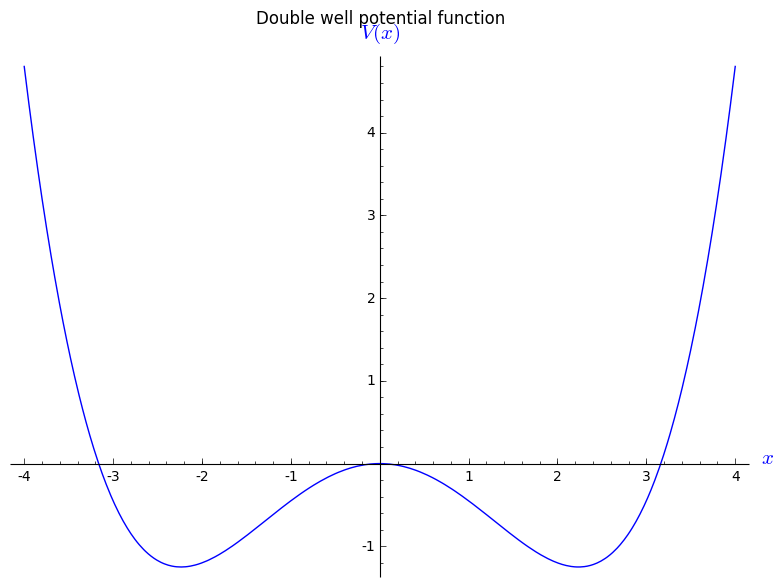
\includegraphics[width=0.6\textwidth]{pics/19_1.png} % INSERIRE QUI LO SCHEMA PER ISING
\caption{Schema di $f_{eff}(m)$ per Ising, $T < T_c$ (doppia buca).}
\label{fig:ch19_1}
\end{figure}

\begin{itemize}
    \item \textbf{Caso continuo (Heisenberg):} Per $T < T_c$, la situazione è diversa. Il sistema si ordina, e la magnetizzazione $\bar{m}_{eq}$ sceglie una direzione specifica nello spazio, rompendo la simmetria rotazionale continua. Tuttavia, tutte le direzioni sono equivalenti energeticamente. Il landscape dell'energia libera $f_{eff}(\bar{m})$ assomiglia a un "cappello messicano" (sombrero). C'è una valle continua di minimi degeneri che corrispondono a tutte le possibili direzioni di $\bar{m}_{eq}$ con lo stesso modulo.
\end{itemize}

\begin{figure}[h!]
\centering
% 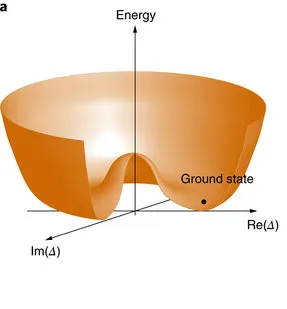
\includegraphics[width=0.6\textwidth]{pics/19_2.png} % INSERIRE QUI LO SCHEMA PER HEISENBERG
\caption{Schema di $f_{eff}(\bar{m})$ per Heisenberg (2D), $T < T_c$ (cappello messicano).}
\label{fig:ch19_9}
\end{figure}

Le fluttuazioni del modulo della magnetizzazione (salire/scendere le pareti del cappello) sono "dure" (costano energia). Tuttavia, le fluttuazioni lungo la valle dei minimi (cambiamenti nella direzione della magnetizzazione mantenendo il modulo costante) sono "soffici" e non costano energia (o costano molto poco a grandi lunghezze d'onda). Queste fluttuazioni soffici sono chiamate \textbf{modi di Goldstone} e sorgono ogni volta che una simmetria continua viene rotta spontaneamente.
La presenza di modi di Goldstone rende le fluttuazioni più importanti nei sistemi con simmetria continua.

La dimensionalità critica inferiore (la dimensione al di sotto della quale non c'è ordine per $T>0$) può essere più alta. Ad esempio, il modello di Ising ordina per $d \ge 2$, mentre il modello di Heisenberg ordina per $d \ge 3$.
Per $T < T_c$ (non solo a $T_c$), nella fase ordinata, le funzioni di correlazione connesse possono decadere come leggi di potenza a causa di questi modi soffici, invece che esponenzialmente. Questo significa che trovare un decadimento a legge di potenza non implica necessariamente che il sistema sia al punto critico $T_c$; potrebbe essere in una fase a bassa temperatura con rottura di simmetria continua.


\section{Calcolo Approssimato della Funzione di Correlazione per $T \ll T_c$ (Modi di Goldstone)}
Consideriamo un modello con simmetria continua (es. Heisenberg) a temperature molto basse rispetto a $T_c$, dove il sistema è fortemente ordinato.
L'Hamiltoniana è $H = -J \sum_{ij} m_{ij} \bar{S}_i \cdot \bar{S}_j$ dove $m_{ij}=1$ per primi vicini e 0 altrimenti.
La funzione di partizione è data da:

\begin{align*}
Z &= \int d\bar{S} e^{-\beta H(s)} \quad \quad \quad \quad \quad \bar{S} = \{\bar{S}_1, \dots, \bar{S}_N\} \\ 
&= \int d\bar{S} e^{+\beta J \sum \bar{S}_i \cdot \bar{S}_j} \delta(S_i^2 - 1)
\end{align*}

In questa fase, la magnetizzazione globale $\langle \bar{S} \rangle$ punta in una certa direzione, diciamo $\hat{n}$. Ogni spin locale $\bar{S}_i$ sarà quasi allineato con $\hat{n}$, ma avrà piccole fluttuazioni trasversali $\bar{\pi}_i$. Possiamo scrivere:

\begin{equation} \label{eq:ch19_31}
\bar{S}_i = S_i^L \hat{n} + \bar{\pi}_i
\end{equation}

dove $S_i^L$ è la componente longitudinale e $\bar{\pi}_i \cdot \hat{n} = 0$. Poiché $|\bar{S}_i|^2 = 1$, abbiamo:
$(S_i^L)^2 + |\bar{\pi}_i|^2 = 1$.
Per $\pi_i = |\bar{\pi}_i| \ll 1$ (piccole fluttuazioni trasversali), possiamo approssimare la componente longitudinale:

\begin{equation} \label{eq:ch19_32}
S_i^L = \sqrt{1 - \pi_i^2} \approx 1 - \frac{\pi_i^2}{2}
\end{equation}

Sostituendo questo nell'Hamiltoniana e sviluppando $\bar{S}_i \cdot \bar{S}_j$ fino ai termini quadratici in $\pi$:

\begin{align*} 
\bar{S}_i \cdot \bar{S}_j &= S_i^L S_j^L + \bar{\pi}_i \cdot \bar{\pi}_j \\ 
&\approx \left(1-\frac{\pi_i^2}{2}\right)\left(1-\frac{\pi_j^2}{2}\right) + \bar{\pi}_i \cdot \bar{\pi}_j \\ 
&\approx 1 - \frac{\pi_i^2}{2} - \frac{\pi_j^2}{2} + \bar{\pi}_i \cdot \bar{\pi}_j 
\end{align*}

L'Hamiltoniana (ignorando i termini costanti) diventa un'Hamiltoniana quadratica per i campi $\bar{\pi}_i$, che rappresentano le fluttuazioni trasversali (modi di Goldstone).

\begin{equation} \label{eq:ch19_33}
H \approx \text{const} + J \sum_{ij} m_{ij} \left( -\pi_i^2 + \bar{\pi}_i \cdot \bar{\pi}_j \right)
\end{equation}

(considerando la simmetria di $m_{ij}$ e che i termini $\sum \pi_i^2$ e $\sum \pi_j^2$ danno lo stesso contributo).
Questa può essere riscritta usando l'operatore Laplaciano discreto $\Lambda_{ij}$:

\begin{equation} \label{eq:ch19_34}
H \approx \sum_{ij} \Lambda_{ij} \bar{\pi}_i \cdot \bar{\pi}_j
\end{equation}

Con:
\begin{equation} \label{eq:ch19_35}
\Lambda_{ij} = -m_{ij} + \delta_{ij} \sum_k m_{ik} 
\end{equation}

Nel limite continuo: $\Lambda_{ij} \rightarrow -L^2 \nabla^2$.
La probabilità di una configurazione $\{\bar{\pi}_i\}$ è data da:

\begin{equation} \label{eq:ch19_36}
P(\{\bar{\pi}_i\}) = \frac{1}{Z} e^{-\beta J \sum \Lambda_{ij} \bar{\pi}_i \cdot \bar{\pi}_j} \; \delta\left(\sum_i \bar{\pi}_i\right)
\end{equation}

dove la $\delta$ rappresenta il vincolo che la somma delle fluttuazioni trasversali non alteri la magnetizzazione globale, $\sum_i \bar{\pi}_i = 0$.
Nello spazio di Fourier, si trova:

\begin{equation} \label{eq:ch19_37}
C^c(\bar{q}) = \frac{1}{Z} \int d\hat{\pi}(\bar{q}) \hat{\pi}(\bar{q}) \hat{\pi}(-\bar{q}) e^{-\beta \sum q^2 |\hat{\pi}(\bar{q})|^2} \delta(\hat{\pi}(0))
\end{equation}

Essendo l'Hamiltoniana Gaussiana, il calcolo della funzione di correlazione per questi modi è standard. La funzione di correlazione per i modi di Goldstone nello spazio di Fourier risulta essere:

\begin{equation} \label{eq:ch19_38}
C^c(\bar{q}) \sim \frac{1}{q^2} \quad (\text{per } q \neq 0)
\end{equation}

Antitrasformando questa espressione per ottenere la funzione di correlazione nello spazio reale, si ottiene:

\begin{equation} \label{eq:ch19_39}
C^c(\bar{r}_{ij}) = \int d\bar{\pi}_i \delta\left(\sum_k \bar{\pi}_k\right) e^{-\beta J \sum_{kl} \Lambda_{kl} \bar{\pi}_k \cdot \bar{\pi}_l} (\bar{\pi}_i \cdot \bar{\pi}_j)
\end{equation}

È un decadimento a legge di potenza. In $d$ dimensioni:

\vspace{0.5cm}
\noindent\fbox{%
    \parbox{\dimexpr\linewidth-2\fboxsep-2\fboxrule\relax}{%
        \begin{equation} \label{eq:ch19_40}
        C^c(r) \sim \frac{1}{r^{d-2}}
        \end{equation}
    }%
}
\vspace{0.5cm}

Per $d=3$, questo dà $C^c(r) \sim \frac{1}{r}$.
Questo dimostra come i modi di Goldstone, presenti nella fase ordinata ($T < T_c$) di un sistema con simmetria continua rotta spontaneamente, portino a correlazioni a lungo raggio (decadimento a legge di potenza) anche lontano dal punto critico $T_c$. Le fluttuazioni $\bar{\pi}_i$ sono direttamente collegate a piccole rotazioni della magnetizzazione globale, e quindi rappresentano i modi di Goldstone.

%-------------------------------------------------------------------------------
% CAPITOLO 20
%-------------------------------------------------------------------------------
\chapter{Lezione 20}
\label{capitolo_20}
\textit{13/05/2026}

\section{Potenziale di Membrana}
Il potenziale d'azione nei neuroni è una variazione rapida del potenziale di membrana che si verifica in un breve lasso di tempo. Per comprendere questo fenomeno, è necessario analizzare il comportamento della membrana cellulare e dei canali ionici che la attraversano.
La membrana cellulare del neurone, come in altre cellule, è costellata di canali ionici. Un singolo neurone può possedere diversi tipi di canali ionici, ad esempio 8 o 9 tipi, e nell'intero sistema nervoso se ne possono trovare centinaia. Questi canali ionici sono proteine che attraversano la membrana e presentano le seguenti caratteristiche:

\begin{itemize}
    \item \textbf{Sono semipermeabili:} permettono il passaggio selettivo di ioni tra l'interno e l'esterno della cellula.
    \item \textbf{Sono selettivi:} ogni tipo di canale è specifico per determinati ioni (es. canali per il Calcio, canali per il Potassio\dots).
\end{itemize}

A causa di questa semipermeabilità selettiva, si crea uno squilibrio di cariche ai due lati della membrana, generando una differenza di potenziale di membrana. Gli ioni si muovono attraverso la membrana spinti da due forze principali:

\begin{itemize}
    \item \textbf{Forza di diffusione:} dovuta a gradienti di concentrazione. Se la concentrazione di uno ione è maggiore da un lato della membrana (es. interno) rispetto all'altro (es. esterno), gli ioni tenderanno a muoversi verso la regione a minore concentrazione.
    \item \textbf{Forza elettrica:} dovuta alla differenza di potenziale elettrico attraverso la membrana. Questa forza si oppone o favorisce il movimento degli ioni a seconda della loro carica e del campo elettrico.
\end{itemize}

All'equilibrio, queste due forze si bilanciano. In una situazione di solo equilibrio diffusionale, la differenza di potenziale di membrana si attesta intorno ai $50 \text{ mV}$.


\section{Pompe Ioniche}
Oltre ai meccanismi passivi di diffusione e forza elettrica, esistono proteine chiamate pompe ioniche. Queste pompe trasportano attivamente ioni contro il loro gradiente elettrochimico, mantenendo il potenziale di membrana a un valore stazionario diverso da quello di equilibrio puramente diffusionale. Questo processo richiede energia e genera una corrente ionica netta. In presenza delle pompe ioniche, la differenza di potenziale attraverso un singolo canale ionico può raggiungere valori dell'ordine di $50-100 \text{ mV}$. Il valore esatto dipende dal tipo specifico di canale ionico considerato.


\section{Modellizzazione della Membrana Come Capacitore}
La membrana cellulare, nel suo complesso, può essere schematizzata come un capacitore, poiché separa cariche elettriche sui suoi due lati. Se $C$ è la capacità dell'intera membrana e $V$ è la differenza di potenziale ai suoi capi, la variazione di potenziale nel tempo è data da:

\begin{equation} \label{eq:ch20_1}
C\frac{dV}{dt} = I_{tot}
\end{equation}

La corrente totale $I_{tot}$ può essere suddivisa in due contributi principali:
\begin{itemize}
    \item $I_{Ch}$: la corrente dovuta al passaggio di ioni attraverso i canali ionici.
    \item $I_{ext}$: una corrente esterna, ad esempio un segnale elettrico proveniente da altri neuroni connessi.
\end{itemize}

Quindi, l'equazione diventa:

\begin{equation} \label{eq:ch20_2}
C\frac{dV}{dt} = I_{Ch} + I_{EXT}
\end{equation}

La corrente attraverso i canali $I_{Ch}$ è la somma dei contributi di tutti i tipi di canali presenti. Se $n$ è il numero di diversi tipi di canali:

\begin{equation} \label{eq:ch20_3}
I_{Ch} = \sum_{i=1}^{n} N_{i}f_{i}g_{i}(V_{i}-V)
\end{equation}

Dove:
\begin{itemize}
    \item $N_i$: è il numero di canali del tipo $i$-esimo sulla membrana (una costante che rappresenta l'abbondanza di quel tipo di canale).
    \item $f_i$: è la frazione di canali del tipo $i$-esimo che sono aperti. Questa frazione dipende dal potenziale di membrana $V$.
    \item $g_i$: è la conduttanza di un singolo canale aperto del tipo $i$-esimo ($g_i = 1/R_i$, dove $R_i$ è la resistenza del canale).
    \item $V_i$: è il potenziale di riposo (o di inversione) per il canale di tipo $i$-esimo. È il valore del potenziale di membrana $V$ al quale la corrente attraverso il canale di tipo $i$ si annulla. Se $V=V_i$, non c'è flusso netto di corrente attraverso quel specifico tipo di canale, anche se potrebbe esserci corrente attraverso altri tipi di canali.
\end{itemize}

Il prodotto $g_i(V_i-V)$ rappresenta la corrente che fluisce attraverso un singolo canale aperto di tipo $i$.


\section{Dinamica della Frazione di Canali Aperti}
La frazione di canali aperti $f_i$ non è costante ma dipende essa stessa dal potenziale $V$. Questa dipendenza è cruciale perché introduce un meccanismo di feedback che permette l'apertura rapida e concertata di molti canali, alla base dell'impulso nervoso.
Si può assumere che $f_i$ tenda a un valore di equilibrio $f_i^{eq}(V)$ che dipende dal potenziale istantaneo $V$. La dinamica con cui $f_i$ si avvicina a questo valore di equilibrio può essere descritta da un'equazione di rilassamento esponenziale:

\begin{equation} \label{eq:ch20_4}
\frac{df_{i}}{dt} = -\frac{1}{\tau_{i}}[f_{i}-f_{i}^{eq}(V)]
\end{equation}

Dove $\tau_i$ è la costante di tempo caratteristica per l'apertura/chiusura dei canali di tipo $i$. Canali diversi possono avere $\tau_i$ diversi (canali rapidi o lenti).
Il sistema completo di equazioni da risolvere è quindi costituito dall'equazione per $dV/dt$ e dalle $n$ equazioni per $df_i/dt$:

\vspace{0.5cm}
\noindent\fbox{%
    \parbox{\dimexpr\linewidth-2\fboxsep-2\fboxrule\relax}{%
        \begin{equation} \label{eq:ch20_5}
        \begin{cases}  
        \frac{df_{i}}{dt} &= -\frac{1}{\tau_{i}}[f_{i}-f_{i}^{eq}(V)] \\ \\ 
        C\frac{dV}{dt} &= \sum_{i=1}^{n} N_{i}f_{i}g_{i}(V_{i}-V) + I_{EXT} 
        \end{cases} 
        \end{equation}
    }%
}
\vspace{0.5cm}


\section{Determinazione di $f_i^{eq}(V)$: Modello a Due Stati}
Per determinare $f_i^{eq}(V)$, consideriamo un singolo canale che può esistere in due stati: aperto (O) o chiuso (C).
Quando un canale si apre, una certa quantità di carica, detta gating charge $Q_{eff}$ (carica efficace, che può essere un multiplo della carica elementare $e$, cioè $Q \cdot e$), si muove attraverso la membrana, che si trova a un potenziale $V$. Questo movimento di carica comporta una variazione dell'energia libera del canale.
Siano $F_{i0}^C$ e $F_{i0}^O$ le energie libere del canale di tipo $i$ rispettivamente nello stato chiuso e aperto, in assenza dell'effetto del potenziale di membrana sulla gating charge.

Quando il potenziale di membrana è $V$:
\begin{itemize}
    \item Energia libera dello stato chiuso: $E_C = F_{i0}^C$
    \item Energia libera dello stato aperto: $E_O = F_{i0}^O - Q_{eff}V$
\end{itemize}

Il termine $-Q_{eff}V$ rappresenta la diminuzione di energia dovuta al movimento della gating charge $Q_{eff}$ secondo il potenziale $V$.
Utilizzando la statistica di Boltzmann, la probabilità che il canale sia aperto, $P_i^O$, che corrisponde a $f_i^{eq}(V)$, è data da:

\begin{equation} \label{eq:ch20_6}
P_i^O = \frac{e^{-\beta E_O}}{e^{-\beta E_O} + e^{-\beta E_C}} = \frac{e^{-\beta (F_{i0}^O - Q_{eff}V)}}{e^{-\beta (F_{i0}^O - Q_{eff}V)} + e^{-\beta F_{i0}^C}}
\end{equation}

Questa espressione può essere riscritta dividendo numeratore e denominatore per $e^{-\beta (F_{i0}^O - Q_{eff}V)}$:

\begin{equation} \label{eq:ch20_7}
P_i^O  = \frac{1}{1 + e^{\beta [F_{i0}^O - F_{i0}^C - Q_{eff}V]}}
\end{equation}

Questa è una funzione sigmoidale e può essere espressa nella forma standard:

\vspace{0.5cm}
\noindent\fbox{%
    \parbox{\dimexpr\linewidth-2\fboxsep-2\fboxrule\relax}{%
        \begin{equation} \label{eq:ch20_8}
        f_i^{eq}(V) = P_i^O(V) = \frac{1}{1+e^{-\frac{(V-V_{1/2,i})}{\Delta_i}}}
        \end{equation}
    }%
}
\vspace{0.5cm}

Dove:
\begin{itemize}
    \item $V_{1/2,i} = \frac{F_{i0}^C - F_{i0}^O}{Q_{eff}}$ è il potenziale al quale metà dei canali di tipo $i$ sono aperti ($f_i^{eq}(V_{1/2,i}) = 1/2$).
    \item $\Delta_i = \frac{1}{Q_{eff}\beta}$ è un parametro che determina la pendenza della curva sigmoidale, rappresentando una scala di potenziale per la sensibilità del canale.
\end{itemize}

La funzione $f_i^{eq}(V)$ è quindi non lineare, il che rende il sistema di equazioni differenziali accoppiate difficile da risolvere analiticamente in generale.

\begin{figure}[h!]
\centering
% 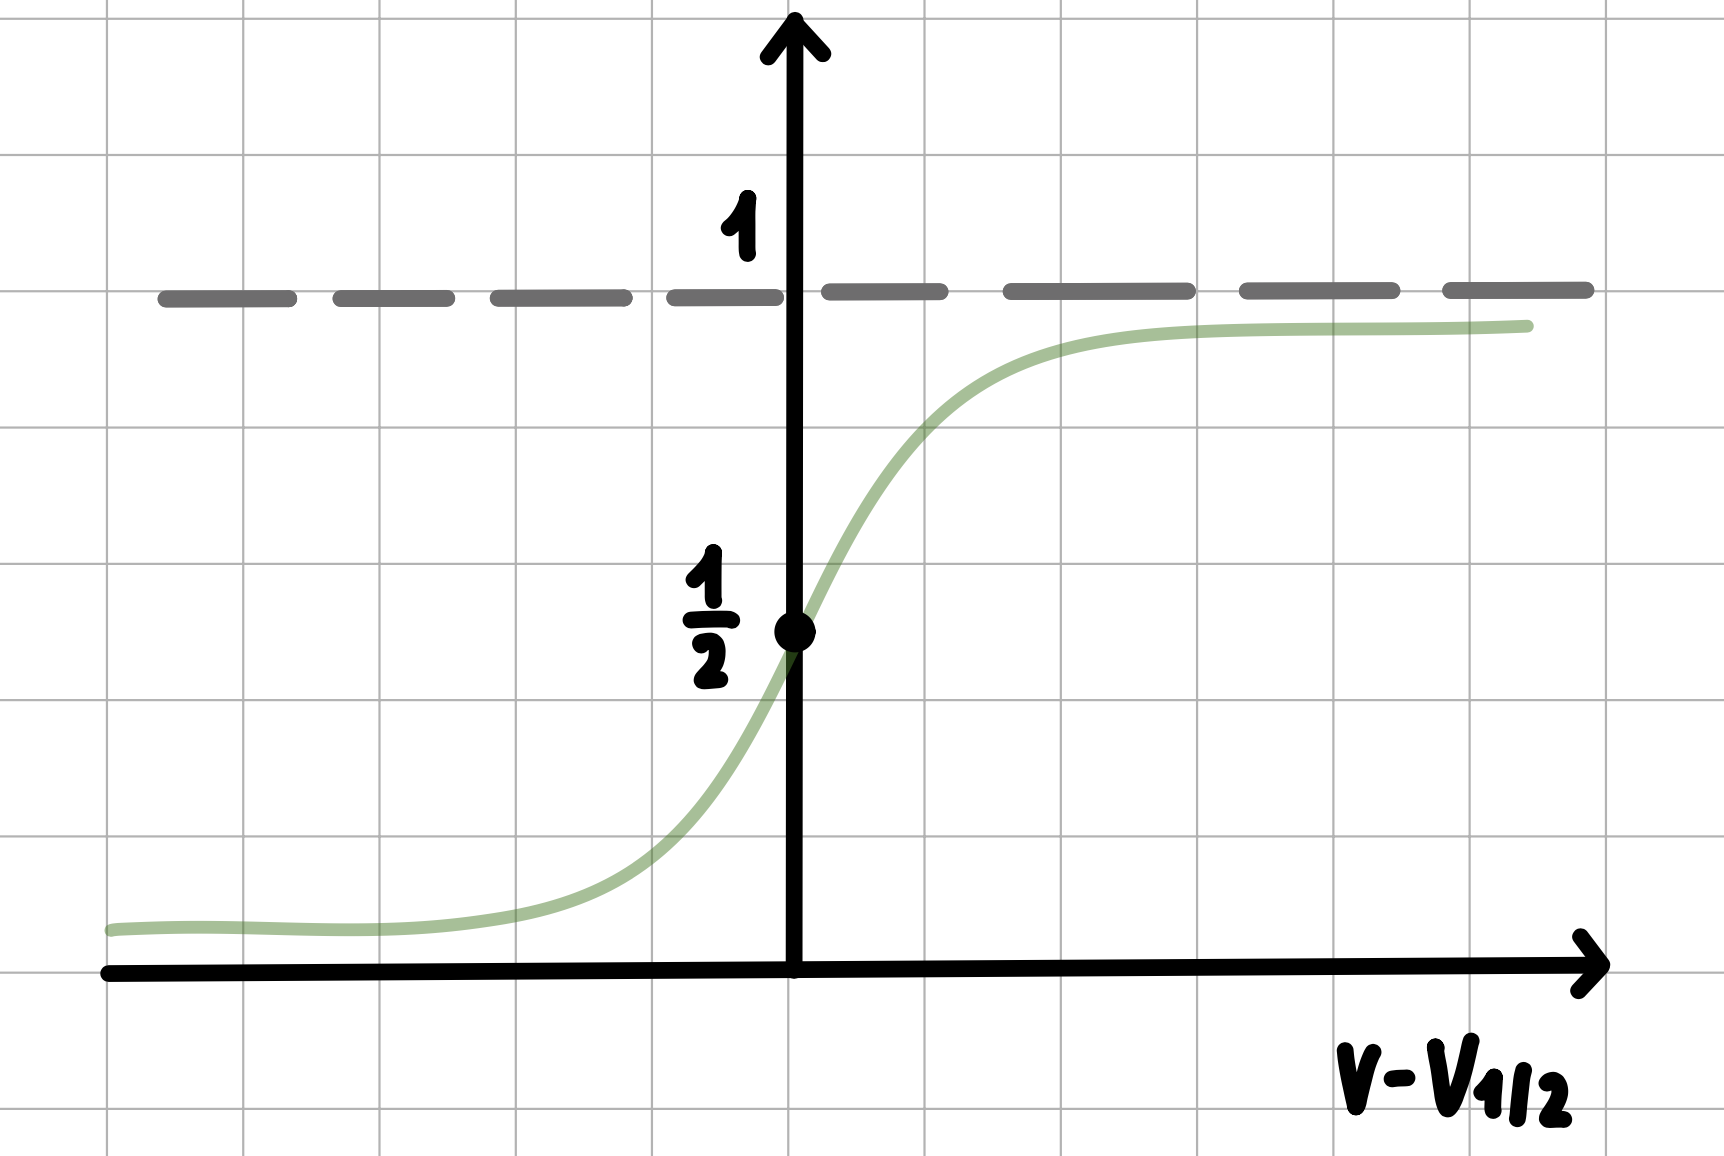
\includegraphics[width=0.6\textwidth]{pics/20_1.png} % INSERIRE QUI IL GRAFICO DELLA FUNZIONE SIGMOIDE
\caption{Curva sigmoidale che descrive la frazione di canali aperti all'equilibrio $f_i^{eq}(V)$ in funzione del potenziale di membrana $V$.}
\label{fig:ch20_1}
\end{figure}


\section{Linearizzazione del Sistema}
Per analizzare il comportamento del sistema, si può ricorrere a una linearizzazione attorno a uno stato stazionario. Assumiamo che il sistema si trovi inizialmente in uno stato stazionario $V_0$ (in assenza di segnali esterni, $\delta I_{EXT}=0$). Applichiamo una piccola perturbazione $\delta I_{EXT}$ che causa piccole variazioni $\delta V$ e $\delta f_i$:

\begin{equation} \label{eq:ch20_9}
\begin{cases}
V(t) &= V_0 + \delta V(t) \\ 
f_i(t) &= f_{i0} + \delta f_i(t) \\ 
f_{i0} &= f_i^{eq}(V_0) 
\end{cases}
\end{equation}

Espandiamo $f_i^{eq}(V)$ attorno a $V_0$:

\begin{equation} \label{eq:ch20_10}
f_i^{eq}(V_0 + \delta V) \approx f_i^{eq}(V_0) + \left.\frac{\partial f_i^{eq}}{\partial V}\right|_{V_0} \delta V 
\end{equation}

Sostituiamo nelle equazioni originali (\ref{eq:ch20_5}):

Per $dV/dt$, si parte da:

\begin{equation} \label{eq:ch20_11}
C\frac{d\delta V}{dt} = \sum_{i=1}^{n}N_{i}g_{i}(f_{i0}+\delta f_{i})[V_{i}-(V_{0}+\delta V)]+I_{EXT}
\end{equation}

Espandendo i prodotti:

\begin{equation*}
C\frac{d\delta V}{dt} = \sum_{i=1}^{n}N_{i}g_{i}(f_{i0}(V_i-V_{0}) - f_{i0}\delta V + \delta f_{i}(V_i-V_{0}) - \delta f_{i}\delta V) + I_{EXT}
\end{equation*}

Nello stato stazionario $V_0$, in assenza di perturbazione esterna ($I_{EXT,0}=0$), si ha:

\begin{equation} \label{eq:ch20_12}
0 = \sum_{i}N_{i}g_{i}f_{i0}(V_{i}-V_{0})
\end{equation}

Trascurando i termini del secondo ordine (come $\delta f_i \delta V$), l'equazione linearizzata per $\delta V$ (con $\delta I$ indicante la perturbazione $I_{EXT}$) è:

\begin{equation} \label{eq:ch20_13}
C\frac{d\delta V}{dt} = \sum_{i=1}^{n}N_{i}g_{i}[-f_{i}^{eq}(V_{0})\delta V + (V_{i}-V_{0})\delta f_{i}] + \delta I
\end{equation}

Per $df_i/dt$, si parte da:

\begin{equation} \label{eq:ch20_14}
\frac{d\delta f_{i}}{dt} = -\frac{1}{\tau_{i}}\Bigg[(f_{i0}+\delta f_{i})-\left(f_{i}^{eq}(V_{0})+\left.\frac{\partial f_{i}^{eq}}{\partial V}\right|_{V_{0}}\delta V\right)\Bigg]
\end{equation}

Che si semplifica a:

\begin{equation} \label{eq:ch20_15}
\frac{d\delta f_{i}}{dt} = -\frac{1}{\tau_{i}}\left[\delta f_{i} - \left.\frac{\partial f_{i}^{eq}}{\partial V}\right|_{V_{0}}\delta V\right]
\end{equation}


\section{Analisi nel Dominio di Fourier}
Per risolvere questo sistema di equazioni differenziali lineari, passiamo al dominio di Fourier.
Definiamo la trasformata di Fourier di una funzione $x(t)$ come:
$\hat{x}(\omega) = \int x(t)e^{i\omega t}dt$
La derivata $dx/dt$ si trasforma in $-i\omega \hat{x}(\omega)$

Le equazioni linearizzate trasformate diventano:

\begin{equation} \label{eq:ch20_16}
-i\omega C \delta\hat{V}(\omega) = -\sum_{i}N_ig_{i}f_{i0}\delta\hat{V}(\omega) + \sum_{i}N_ig_{i}(V_{i}-V_{0})\delta\hat{f}_{i}(\omega) + \delta\hat{I}(\omega)
\end{equation}

\begin{equation} \label{eq:ch20_17}
-i\omega\delta\hat{f}_{i}(\omega) = -\frac{1}{\tau_{i}}\left[\delta\hat{f}_{i}(\omega) - \left.\frac{df_{i}^{eq}}{dV}\right|_{V_{0}}\delta\hat{V}(\omega)\right]
\end{equation}

Dalla seconda equazione, possiamo esprimere $\delta\hat{f}_{i}(\omega)$ in termini di $\delta\hat{V}(\omega)$:

\begin{equation} \label{eq:ch20_18}
\delta\hat{f}_{i}(\omega) = \frac{1}{1-i\omega\tau_{i}}\left.\frac{df_{i}^{eq}}{dV}\right|_{V_{0}}\delta\hat{V}(\omega)
\end{equation}

Sostituendo questa espressione nella (\ref{eq:ch20_16}):

\begin{align*} 
-i\omega C \delta\hat{V}(\omega) &= -\left(\sum_{i}N_ig_{i}f_{i0}\right)\delta\hat{V}(\omega) \\
&+ \sum_{i}N_ig_{i}(V_{i}-V_{0})\frac{1}{1-i\omega\tau_{i}}\left.\frac{df_{i}^{eq}}{dV}\right|_{V_{0}}\delta\hat{V}(\omega)\\ 
&+ \delta\hat{I}(\omega) 
\end{align*}

Raccogliendo i termini con $\delta\hat{V}(\omega)$:

\begin{align} \label{eq:ch20_19}
\delta\hat{I}(\omega) = \delta\hat{V}(\omega) \left\{ -i\omega C + \sum_{i}N_ig_{i} \Bigg[ f_{i0} - \frac{(V_{i}-V_{0})}{1-i\omega\tau_{i}}\left.\frac{df_{i}^{eq}}{dV}\right|_{V_{0}} \Bigg]\right\} 
\end{align}

Definendo la conduttanza di base $1/R_0 = \sum_{i}N_ig_{i}f_{i0}$ (la conduttanza totale della membrana nello stato stazionario $V_0$ dovuta alla frazione basale di canali aperti):

\vspace{0.5cm}
\noindent\fbox{%
    \parbox{\dimexpr\linewidth-2\fboxsep-2\fboxrule\relax}{%
        \begin{equation} \label{eq:ch20_20}
        \delta\hat{I}(\omega) = \delta\hat{V}(\omega) \left\{ -i\omega C + \frac{1}{R_{0}} + \sum_{i}N_ig_{i}\frac{(V_{0}-V_{i})}{1-i\omega\tau_{i}}\left.\frac{df_{i}^{eq}}{dV}\right|_{V_{0}} \right\}
        \end{equation}
    }%
}
\vspace{0.5cm}

Questa equazione lega la perturbazione di corrente applicata $\delta\hat{I}(\omega)$ alla risposta in potenziale $\delta\hat{V}(\omega)$ attraverso un'impedenza generalizzata $Z(\omega)$, dove $\delta\hat{V}(\omega) = Z(\omega)\delta\hat{I}(\omega)$.
L'espressione tra parentesi graffe è l'ammettenza $Y(\omega) = 1/Z(\omega)$.


\section{Analisi dei Casi Limite del Termine di Somma}
Il termine $\sum_{i}N_ig_{i}\frac{(V_{0}-V_{i})}{1-i\omega\tau_{i}}\left.\frac{df_{i}^{eq}}{dV}\right|_{V_{0}}$ modifica l'ammettenza del sistema in modo dipendente dalla frequenza.

\subsection*{Canali Veloci ($\tau_i \omega \ll 1$)}
Per canali con costante di tempo $\tau_i$ molto piccola, il termine $1-i\omega\tau_i \approx 1$.
Il contributo all'ammettenza diventa una conduttanza costante:

\begin{equation} \label{eq:ch20_21}
\sum_{i \in \text{veloci}} N_ig_{i}(V_{0}-V_{i})\left.\frac{df_{i}^{eq}}{dV}\right|_{V_{0}}
\end{equation}

Consideriamo le condizioni per un feedback positivo:
\begin{itemize}
    \item $\left.\frac{df_{i}^{eq}}{dV}\right|_{V_{0}} > 0$: un aumento di $V$ apre più canali (sensibilità positiva).
    \item $V_i > V_0$: il potenziale di inversione del canale è maggiore del potenziale di riposo $V_0$. Questo implica che allo stato $V_0$ c'è una forza spingente per l'ingresso di cariche positive (o uscita di negative) se il canale si apre.
\end{itemize}

In queste condizioni, il termine $(V_0 - V_i)$ è negativo. Quindi, il contributo di questi canali alla conduttanza $(V_0-V_i) \cdot (df/dV)$ è \textbf{negativo}. Una conduttanza negativa effettiva riduce la resistenza totale del circuito, potenziando la risposta a una perturbazione (feedback positivo).

\subsection*{Canali Lenti ($\tau_i \omega \gg 1$)}
Per canali con costante di tempo $\tau_i$ molto grande, il termine $1-i\omega\tau_i \approx -i\omega\tau_i$.
Il contributo all'ammettenza diventa:

\begin{equation} \label{eq:ch20_22}
\sum_{i \in \text{lenti}} N_ig_{i}(V_{0}-V_{i})\left.\frac{df_{i}^{eq}}{dV}\right|_{V_{0}} \frac{1}{-i\omega\tau_i} = \frac{1}{i\omega} \sum_{i \in \text{lenti}} N_ig_{i}\frac{(V_{i}-V_{0})}{\tau_{i}}\left.\frac{df_{i}^{eq}}{dV}\right|_{V_{0}}
\end{equation}

Questo termine ha la forma $1/(i\omega L_{eff})$, che è l'ammettenza di un'induttanza efficace $L_{eff}$, dove:

\begin{equation} \label{eq:ch20_23}
L_{eff} = \left( \sum_{i \in \text{lenti}} N_ig_{i}\frac{(V_{i}-V_{0})}{\tau_{i}}\left.\frac{df_{i}^{eq}}{dV}\right|_{V_{0}} \right)^{-1}
\end{equation}

Quindi, i canali lenti possono conferire proprietà \textbf{induttive} alla membrana neuronale a certe frequenze.

Questi comportamenti (conduttanza negativa per canali veloci, induttanza per canali lenti) sono importanti per determinare la risposta dinamica del neurone a segnali variabili nel tempo e possono contribuire a fenomeni come la risonanza e l'eccitabilità neuronale.

%-------------------------------------------------------------------------------
% CAPITOLO 21
%-------------------------------------------------------------------------------
\chapter{Lezione 21}
\label{capitolo_21}
\textit{16/05/2026}

\section{Modello della Membrana Neuronale}
Modelliamo la membrana di un neurone come un condensatore. Sulla membrana sono presenti diversi tipi di canali ionici.
L'equazione che descrive la variazione del potenziale di membrana $V$ nel tempo è data da:

\begin{equation} \label{eq:ch21_1}
C\frac{dV}{dt} = \sum_{i}^{N_{ch}} g_{i}N_{i}f_{i}(V_{i}-V) + I_{ext}
\end{equation}

dove:
\begin{itemize}
    \item $C$ è la capacità della membrana.
    \item $i$ è un indice che specifica il tipo di canale ionico considerato.
    \item $g_i$ è la conduttanza del singolo canale di tipo $i$.
    \item $N_i$ è il numero totale di canali di tipo $i$.
    \item $f_i$ è la frazione di canali di tipo $i$ che sono aperti.
    \item $V_i$ è il potenziale di riposo per quel tipo di canale, ovvero il valore che il potenziale di membrana dovrebbe avere affinché in quello specifico canale non ci sia corrente.
    \item $V$ è la differenza di potenziale attraverso l'intera membrana, determinata da tutti i tipi di canali.
    \item $I_{ext}$ è un contributo esterno alla corrente, ad esempio proveniente da altri neuroni.
\end{itemize}

La dinamica della frazione di canali aperti $f_i$ è descritta da un'equazione di rilassamento:

\begin{equation} \label{eq:ch21_2}
\frac{df_i}{dt} = -\frac{1}{\tau_i}(f_i - f_i^{eq}(V))
\end{equation}

dove $\tau_i$ è la costante di tempo caratteristica del canale $i$ e $f_i^{eq}(V)$ è la frazione di canali aperti all'equilibrio, che dipende dal potenziale di membrana $V$.
L'espressione esplicita di $f_i^{eq}(V)$ può essere derivata da un modello a due stati:

\begin{equation} \label{eq:ch21_3}
f_i^{eq}(V) = \frac{1}{1 + \exp\left(\frac{V-V_{1/2}}{\Delta}\right)}
\end{equation}

dove $V_{1/2}$ è il potenziale al quale metà dei canali sono aperti e $\Delta$ caratterizza la sensibilità al voltaggio. La varianza $\Delta$ è data dalla carica che si muove dall'interno all'esterno della membrana se il canale si apre.

\subsection*{Feedback positivo}
Consideriamo lo stato stazionario del sistema, che chiamiamo $V_0$. Si analizza cosa succede se si perturba lo stato stazionario $V_0$ con una piccola perturbazione $\delta V$.
Linearizzando il sistema di equazioni, si osserva che esiste una classe di canali veloci che contribuisce con una sorta di resistenza negativa, facilitando il passaggio attraverso la membrana.
Questi canali soddisfano le seguenti condizioni:

\textbf{Prima condizione:}
\begin{equation} \label{eq:ch21_4}
f_i^{eq}(V_0) > 0 
\end{equation}

La prima condizione implica che, anche allo stato stazionario (o di riposo) $V_0$, una frazione seppur piccola di questi canali ionici di tipo $i$ è già aperta. Questo è importante perché implica che i canali sono pronti a rispondere a variazioni di potenziale; non sono in uno stato completamente "chiuso" o inattivo dal quale sarebbe più difficile "attivarli". Se $f_i^{eq}(V_0)$ fosse nulla, una piccola depolarizzazione potrebbe non essere sufficiente ad innescare la loro apertura.

\textbf{Seconda condizione:}
\begin{equation} \label{eq:ch21_5}
\left. \frac{df_i^{eq}}{dV}\right|_{V_0} > 0 
\end{equation}

La seconda condizione indica che la frazione di canali di tipo $i$ aperti all'equilibrio aumenta all'aumentare del potenziale di membrana $V$ (cioè, quando la membrana si depolarizza a partire da $V_0$). Una piccola depolarizzazione della membrana, quindi, causerà l'apertura di un numero maggiore di questi canali.

L'effetto combinato di queste due condizioni fa sì che i canali facilitano il passaggio della corrente attraverso la membrana. Ciò indica che i canali forniscono un feedback positivo alla membrana: se il potenziale aumenta rispetto al valore di equilibrio, l'aumento del potenziale innesca l'apertura di questi canali, e l'apertura dei canali spinge il potenziale a un valore maggiore, che innesca l'apertura di ulteriori canali, e così via. Questo spiega l'apertura improvvisa di molti canali e perché il potenziale di membrana cambia molto rapidamente, portando al cosiddetto potenziale d'azione.


\section{Caso Semplificato con Due Tipi di Canali}
Consideriamo un caso semplice con solo due tipi di canali:
\begin{itemize}
    \item \textbf{Canali di leak:} questi canali sono sempre aperti. La loro frazione di apertura è costante e uguale a 1. Si assume un potenziale di inversione $V_i = V_{leak} = 0$ e la loro conduttanza totale è $G_L = g_{\text{leak}}N_{\text{leak}}$.
    \item \textbf{Altri canali (canali attivi):} questi canali sono tutti uguali, con un potenziale di riposo $V_i = V_R$. La loro conduttanza totale è $g \cdot N$, dove $g$ è la conduttanza del singolo canale attivo e $N$ il loro numero totale. Questi sono i canali responsabili del feedback positivo e la loro frazione di apertura dipende dal voltaggio secondo l'equazione:
\end{itemize}

\begin{equation} \label{eq:ch21_6}
\frac{df}{dt} = -\frac{1}{\tau}(f - f^{eq}(V))
\end{equation}

Abbiamo omesso l'indice $i$ poiché c'è solo un tipo di canale attivo.
In questo caso, l'equazione per il potenziale di membrana diventa:

\begin{equation} \label{eq:ch21_7}
C\frac{dV}{dt} = -G_L V + gNf(V_R - V) + I_{ext}
\end{equation}

\subsection*{Stato Stazionario}
Per trovare lo stato stazionario, poniamo le derivate temporali a zero ($dV/dt = 0$ e $df/dt = 0$).
Dall'equazione (\ref{eq:ch21_7}) (assumendo $I_{ext}=0$ per semplicità nello stato stazionario):

\begin{equation} \label{eq:ch21_8}
G_L V = gNf(V_R - V)
\end{equation}

Da cui possiamo esprimere $f$ in funzione di $V$:

\begin{equation} \label{eq:ch21_9}
f = \frac{G_L V}{gN(V_R - V)}
\end{equation}

Dall'equazione (\ref{eq:ch21_6}):

\begin{equation} \label{eq:ch21_10}
f = f^{eq}(V) = \frac{1}{1 + \exp\left(\frac{V-V_{1/2}}{\Delta}\right)}
\end{equation}

Possiamo risolvere graficamente questo sistema cercando le intersezioni delle due curve $f(V)$.

\begin{figure}[h!]
\centering
% 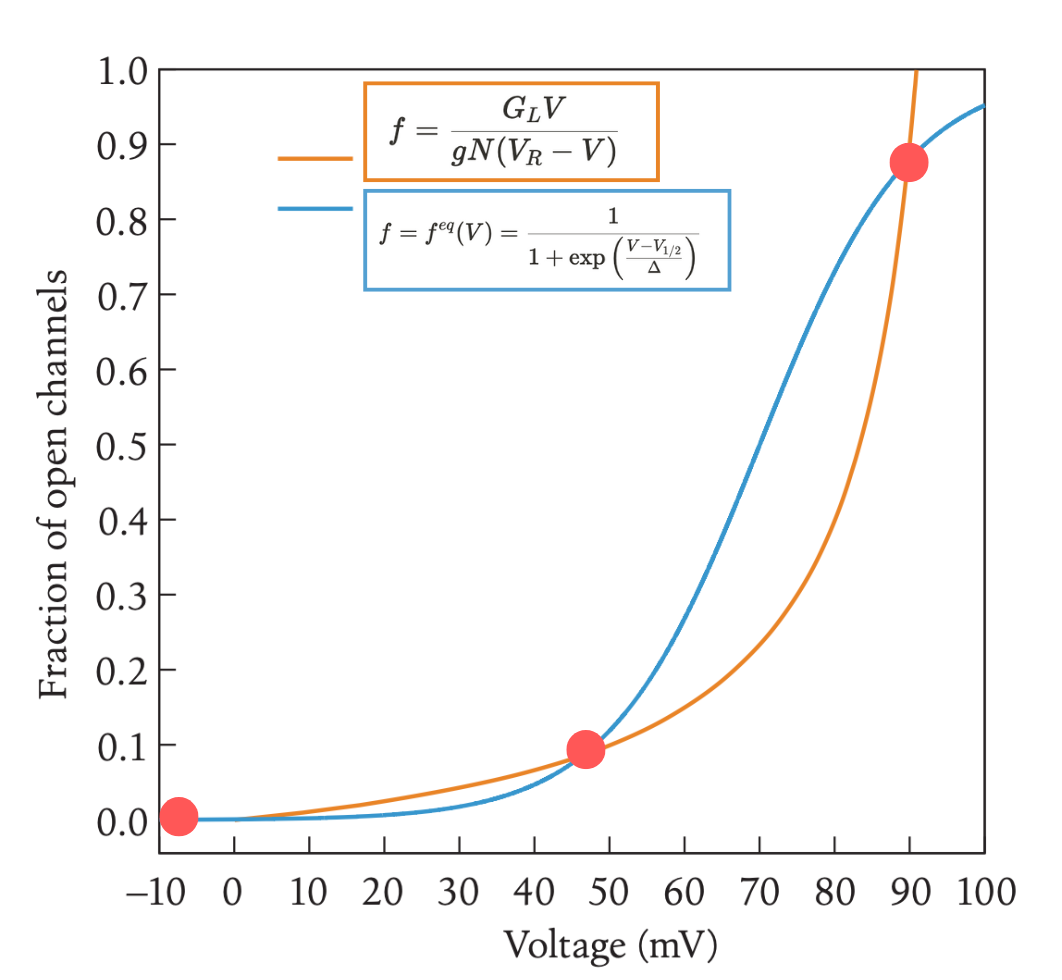
\includegraphics[width=0.6\textwidth]{pics/21_1.png} % INSERIRE QUI IL GRAFICO DELLE INTERSEZIONI DELLE CURVE f(V)
\caption{Risoluzione grafica per lo stato stazionario: intersezioni tra la curva di equilibrio $f^{eq}(V)$ e la curva derivata dalla condizione stazionaria del potenziale.}
\label{fig:ch21_1}
\end{figure}

Si ottengono tre soluzioni: due stabili e una instabile.
\begin{itemize}
    \item \textbf{Uno stato stabile a basso $V$ e basso $f$:} Questo corrisponde allo stato di riposo del neurone. Se il sistema si trova in prossimità di questo punto, piccole perturbazioni lo faranno ritornare a questo stato. In questo stato, la maggior parte dei canali è chiusa (fatta eccezione per quelli di leak).
    \item \textbf{Uno stato instabile a $V$ intermedio.}
    \item \textbf{Uno stato stabile ad alto $V$ e alto $f$:} Questo corrisponde allo stato eccitato del neurone, o al picco del potenziale d'azione, dove una frazione significativa dei canali attivi è aperta.
\end{itemize}

L'evoluzione del sistema è determinata in modo cruciale dalla posizione rispetto al punto di instabilità. Se un impulso di corrente esterna $I_{ext}$ è sufficientemente intenso da elevare il potenziale di membrana $V$ al di sopra del valore corrispondente al punto instabile, il sistema non ritorna più allo stato di riposo. Si attiva, invece, un processo evolutivo a cascata:

\begin{enumerate}
    \item Il nuovo valore di $V$, ora superiore alla soglia di instabilità, porta il sistema a cercare una nuova frazione di equilibrio di canali aperti $f$, come dettato dalla curva $f^{eq}(V)$. Questa frazione $f$ risulterà maggiore di quella associata al punto instabile.
    \item Questa maggiore frazione di canali aperti $f$, a sua volta, induce una variazione del potenziale di membrana $V$, che tenderà verso il valore imposto dalla relazione stazionaria $f(V)$. Questo nuovo valore di $V$ sarà ulteriormente incrementato.
    \item Tale sequenza iterativa, in cui lo stato del sistema si sposta alternativamente tra le condizioni imposte dalle due curve di stazionarietà, prosegue, spingendo progressivamente il sistema verso il secondo punto stabile, caratterizzato da un elevato potenziale $V$ e una grande frazione di canali attivi aperti.
\end{enumerate}

In caso contrario, se la perturbazione non supera la soglia di instabilità, il sistema ritorna allo stato di riposo iniziale.
Questa analisi grafica illustra in modo esplicito l'effetto di feedback positivo e come una perturbazione sopra soglia possa innescare il potenziale d'azione, portando il neurone dallo stato di riposo a quello eccitato.

\begin{figure}[h!]
\centering
% 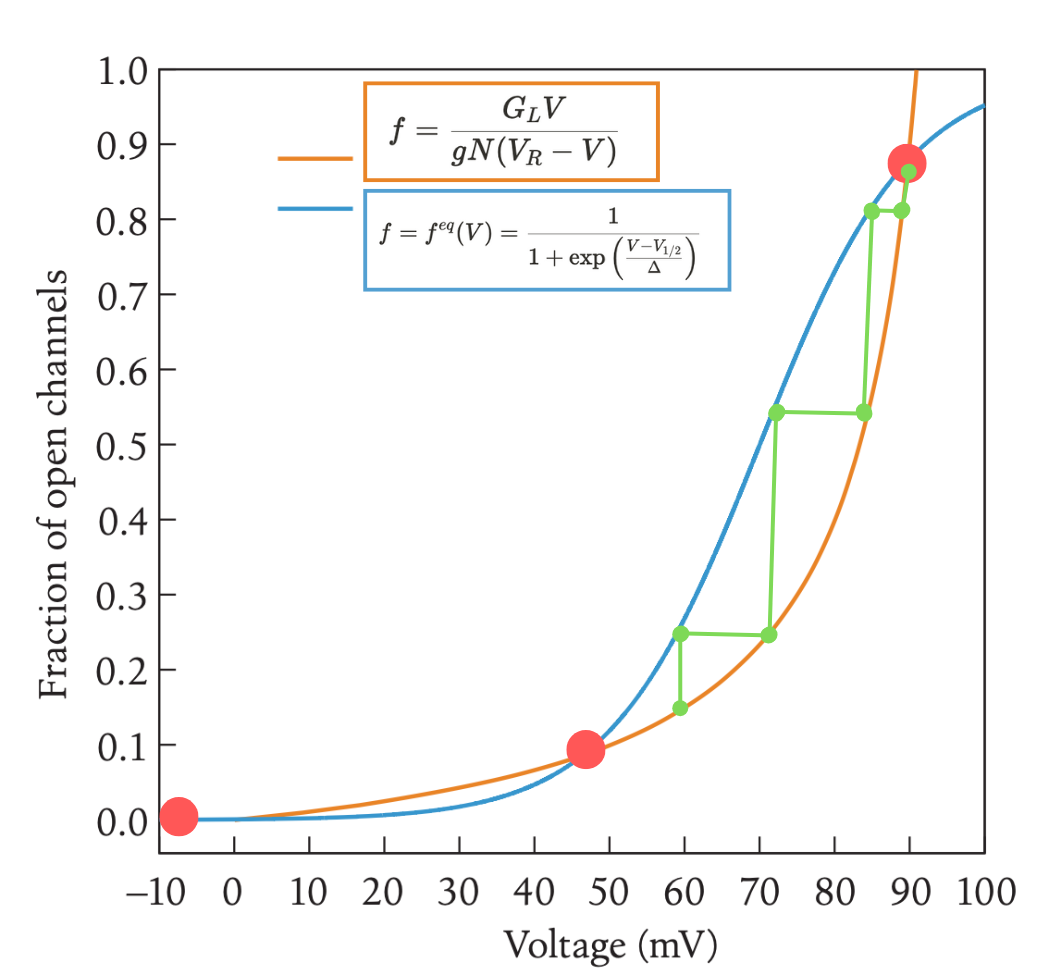
\includegraphics[width=0.6\textwidth]{pics/21_2.png} % INSERIRE QUI IL GRAFICO DELLE INTERSEZIONI DELLE CURVE f(V)
\caption{Effetto di feedback positivo.}
\label{fig:ch21_2}
\end{figure}

\section{Modelli Neuronali Più Realistici}
La descrizione precedente è semplificata. Modelli più realistici dei neuroni includono ulteriori complessità:
\begin{itemize}
    \item \textbf{Porte dei canali (gates):} Si assume che ogni canale abbia diversi gates (attivazione e inattivazione) e che il canale si apra solo quando tutti i gates rilevanti sono aperti. La frazione di canali aperti $f_i$ viene espressa in termini di frazioni di questi gates:
\end{itemize}

\begin{equation} \label{eq:ch21_11}
f_i = m_i^{\alpha_i} h_i^{\beta_i}
\end{equation}

dove $m_i$ è la frazione di gates di attivazione aperti e $h_i$ è la frazione di gates di inattivazione aperti. Per $m_i$ e $h_i$ si scrivono equazioni dinamiche simili a quella per $f_i$.

\begin{itemize}
    \item \textbf{Dipendenza spaziale del potenziale:} Il potenziale di membrana $V$ può variare non solo nel tempo ma anche lungo la posizione $z$ dell'assone del neurone.
\end{itemize}

\begin{equation} \label{eq:ch21_12}
V \equiv V(z,t)
\end{equation}

Includendo questi dettagli si ottengono le equazioni di Hodgkin-Huxley, che possono descrivere la propagazione degli impulsi lungo l'assone.


\section{Reti Neurali}
Dopo aver analizzato la dinamica del singolo neurone, che si caratterizza per processi di trasmissione del segnale molto rapidi, ci si concentra ora sul comportamento collettivo di molti neuroni interconnessi. L'idea di base è che un singolo neurone, in assenza di stimoli significativi, si trovi in uno stato di quiescenza (silente). Tuttavia, riceve continuamente segnali da numerosi altri neuroni con cui è connesso. Quando il segnale cumulativo in ingresso supera una certa soglia critica, il neurone si attiva e genera un potenziale d'azione.

Per modellare una rete di neuroni, si assegna a ciascun neurone $i$ una variabile binaria $S_i$:
\begin{itemize}
    \item $S_i = +1$: stato attivo.
    \item $S_i = -1$: stato silente.
\end{itemize}

L'idea è che un neurone $i$ si attivi se il segnale cumulativo che riceve dagli altri neuroni $S_j$ (pesato dalle connessioni sinaptiche $W_{ij}$) supera una soglia $\vartheta_i$:

\begin{equation} \label{eq:ch21_13}
S_i= \text{sgn}\left(\sum_j W_{ij}S_j- \vartheta_i\right)
\end{equation}

dove $\text{sgn}(x)$ è la funzione segno che restituisce $+1$ se $x > 0$ e $-1$ se $x < 0$.
I pesi sinaptici $W_{ij}$ codificano la forza dell'influenza del neurone $j$ sul neurone $i$. $W_{ij}$ può essere nullo se non c'è connessione diretta, oppure può assumere valori diversi indicanti connessioni più o meno forti, a seconda, ad esempio, del numero di contatti sinaptici tra l'assone di $j$ e i dendriti di $i$.
Questa equazione ricorda l'equazione di campo medio per il modello di Ising a temperatura zero.
L'equazione di campo medio per il modello di Ising è:

\begin{equation} \label{eq:ch21_14}
m_i = \tanh\left(\beta h_i + \beta J \sum_j M_{ij}m_j\right)
\end{equation}

dove $m_i$ è la magnetizzazione locale, $h_i$ il campo esterno locale, $J$ la costante di accoppiamento, $M_{ij}$ la matrice di interazione e $\beta = 1/(k_B T)$.
A temperatura $T \to 0$, la funzione tangente iperbolica $\tanh(\beta x)$ diventa una funzione a gradino, equivalente alla funzione segno $\text{sgn}(x)$; l'equazione (\ref{eq:ch21_14}) diventa:

\begin{equation} \label{eq:ch21_15}
m_i = \text{sgn} \left(\beta h_i + \beta J \sum_j M_{ij}m_j\right)
\end{equation}

Quindi, l'equazione per l'attivazione neuronale è analoga a un modello di Ising a $T=0$.
Questa analogia suggerisce che sia possibile definire una Hamiltoniana per la rete neurale, tale che gli stati stabili della dinamica neuronale corrispondano ai minimi di questa energia.
Per analogia con l'Hamiltoniana del modello di Ising, si può postulare un'Hamiltoniana per la rete neurale della forma:

\begin{equation} \label{eq:ch21_16}
H_N = -\frac{1}{2}\sum_{i, j} W_{ij}S_iS_j + \sum_i \vartheta_i S_i
\end{equation}


\section{Modellare la Memoria}
L'obiettivo primario nello studio di tali reti neurali è comprendere come possano immagazzinare e recuperare informazioni, ovvero come possano funzionare da memorie associative.
L'idea centrale è che la memoria corrisponda a un pattern specifico di attività neuronale, cioè una particolare configurazione degli stati $\{S_i\}$ dei neuroni della rete.
Indichiamo un pattern di memoria con $\{\xi_i^\mu\}$, dove $\xi_i^\mu = \pm 1$ per ogni neurone $i$, e $\mu$ è un indice che etichetta i diversi pattern memorizzati.
Il requisito fondamentale è che questi pattern di memoria siano stati stabili della dinamica della rete. Ciò significa che se la rete viene posta in una configurazione $\{S_i\}$ vicina a un pattern memorizzato, la sua evoluzione dinamica dovrebbe portarla a convergere precisamente a quel pattern (non ad un mix di due diversi pattern) e a rimanervi:

\begin{equation*}
\{S_i\} \longrightarrow  \{\xi_i^\mu\} 
\end{equation*}

In termini dell'analogia con i sistemi fisici, si desidera che i pattern di memoria $\{\xi_i^\mu\}$ corrispondano a minimi locali del landscape energetico definito dall'Hamiltoniana $H_N$.
La questione cruciale è come scegliere i pesi sinaptici $W_{ij}$ (e le soglie $\vartheta_i$, che per semplicità iniziale si pongono uguali a zero) affinché la rete esibisca i pattern desiderati come stati stabili.

\begin{itemize}
    \item \textbf{Modello di Ising ferromagnetico:} Una prima ipotesi, mutuata direttamente dal modello di Ising ferromagnetico, potrebbe essere quella di porre tutti i $W_{ij}$ uguali a una costante positiva $J$. Tuttavia, un tale sistema avrebbe solo due stati fondamentali stabili: quello con tutti i neuroni attivi ($S_i = +1$ per ogni $i$) e quello con tutti i neuroni silenti ($S_i = -1$ per ogni $i$). Questo limiterebbe drasticamente la capacità di memoria a soli due pattern molto specifici, il che è chiaramente insufficiente.
    \item \textbf{Modello di vetro di spin:} Un'alternativa opposta sarebbe scegliere i $W_{ij}$ in modo casuale. Questo porta a un modello noto come "spin glass" (vetro di spin). I vetri di spin sono caratterizzati da un fenomeno chiamato "frustrazione": a causa della natura disordinata e competitiva delle interazioni (alcune positive, altre negative), non è possibile soddisfare simultaneamente tutti i legami energetici.
\end{itemize}

Un semplice esempio di frustrazione si ha in un reticolo triangolare di spin con interazioni antiferromagnetiche: se due spin adiacenti sono anti-allineati per minimizzare la loro energia, il terzo spin non può soddisfare contemporaneamente il legame con entrambi.

\begin{figure}[h!]
\centering
% 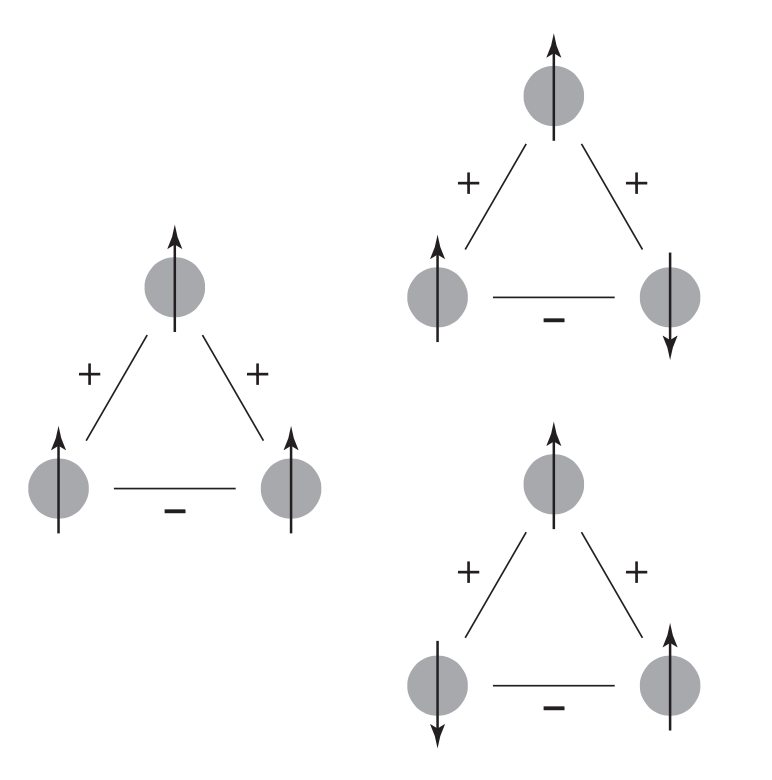
\includegraphics[width=0.4\textwidth]{pics/21_3.png} % INSERIRE QUI LO SCHEMA DELLA FRUSTRAZIONE (ES. TRIANGOLO ANTIFERROMAGNETICO)
\caption{Esempio di frustrazione in un reticolo triangolare con interazioni antiferromagnetiche.}
\label{fig:ch21_3}
\end{figure}

La conseguenza della frustrazione è un landscape energetico estremamente complesso, con un numero elevatissimo di minimi locali sub-ottimali, molti dei quali possono avere energie simili.
Se da un lato la presenza di molti minimi potrebbe sembrare vantaggiosa per immagazzinare numerosi pattern, i vetri di spin presentano un problema significativo: la posizione esatta di questi minimi nello spazio delle configurazioni è estremamente sensibile a piccole variazioni nei valori dei $W_{ij}$. Questa fragilità rende i vetri di spin inadatti come modello per una memoria robusta, poiché la perdita o l'alterazione di poche connessioni sinaptiche potrebbe stravolgere l'intera struttura delle memorie immagazzinate.
Si cerca quindi una via intermedia tra l'eccessiva semplicità del modello ferromagnetico e l'eccessiva fragilità dei vetri di spin.


\section{Il Modello di Hopfield}
Il modello di Hopfield, introdotto negli anni '80, fornisce una prescrizione specifica per costruire i pesi sinaptici $W_{ij}$ in modo che una serie di $K$ pattern di memoria desiderati $\{\vec{\xi}^\mu\}_{\mu=1}^K$ diventino minimi di energia.
Supponiamo di voler memorizzare un singolo pattern generico $\vec{\xi} = (\xi_1, \xi_2, \dots, \xi_N)$, dove ogni $\xi_i = \pm 1$.
L'idea di Hopfield è di definire i pesi sinaptici come:

\begin{equation} \label{eq:ch21_17}
W_{ij} =  \xi_i \xi_j W
\end{equation}

Con questa scelta, l'Hamiltoniana (assumendo $\vartheta_i=0$) diventa:

\begin{equation} \label{eq:ch21_18}
H = -\frac{1}{2} \sum_{i, j} W_{ij}S_iS_j = -\frac{W}{2} \sum_{i,j} (\xi_i \xi_j) S_i S_j
\end{equation}

Questa espressione può essere riscritta introducendo nuove variabili $S'_i = S_i \xi_i$.
Poiché $\xi_i = \pm 1$, anche $S'_i = \pm 1$.
Sostituendo:

\begin{equation} \label{eq:ch21_19}
H = -\frac{W}{2}\sum_{i,j} S'_i S'_j
\end{equation}

Questa è l'Hamiltoniana di un modello di Ising con interazione a lungo raggio (ogni $S'_i$ interagisce con ogni $S'_j$) con costante di accoppiamento $W$.
Gli stati di minima energia per tale sistema si hanno quando tutti gli $S'_i$ sono allineati:

\begin{itemize}
    \item $S'_i = +1$ per tutti gli $i \implies S_i \xi_i = +1 \implies S_i = \xi_i$ (poiché $1/\xi_i = \xi_i$)
    \item $S'_i = -1$ per tutti gli $i \implies S_i \xi_i = -1 \implies S_i = -\xi_i$
\end{itemize}

Dunque, i due stati di minima energia della rete sono esattamente il pattern $\vec{\xi}$ e il suo opposto.

\vspace{0.5cm}
\noindent\fbox{%
    \parbox{\dimexpr\linewidth-2\fboxsep-2\fboxrule\relax}{%
        La rete è in grado di memorizzare un pattern generico $\vec{\xi}$, non solo configurazioni uniformi come nel caso ferromagnetico semplice.
    }%
}
\vspace{0.5cm}

Un modo alternativo per visualizzare l'energia, è notare che $H$ è proporzionale a $-(\vec{\xi} \cdot \vec{S})^2$:

\begin{equation} \label{eq:ch21_20}
H = -C (\vec{\xi} \cdot \vec{S})^2
\end{equation}

dove $C$ è una costante positiva. L'energia è minimizzata quando il prodotto scalare tra lo stato della rete $\vec{S}$ e il pattern memorizzato $\vec{\xi}$ è massimo in valore assoluto, cioè quando $\vec{S} = \pm\vec{\xi}$.

Consideriamo il caso di due pattern distinti, $\vec{\xi}^1 = \{\xi_i^1\}$ e $\vec{\xi}^2 = \{\xi_i^2\}$.
I pesi sinaptici $W_{ij}$ vengono costruiti come la somma dei contributi individuali di ciascun pattern:

\begin{equation} \label{eq:ch21_21}
W_{ij} = W(\xi_i^1 \xi_j^1 + \xi_i^2 \xi_j^2)
\end{equation}

Assumendo $W_{ii}=0$. Sostituendo questa espressione dei pesi nell'Hamiltoniana generale $H = -\frac{1}{2}\sum_{i \neq j} W_{ij}S_iS_j$, l'energia del sistema in funzione della configurazione di spin $\vec{S}$ e dei due pattern memorizzati assume la forma:

\begin{equation} \label{eq:ch21_22}
H = -\frac{W}{2}\left[ (\vec{\xi}^1 \cdot \vec{S})^2 + (\vec{\xi}^2 \cdot \vec{S})^2 \right]
\end{equation}

Questa espressione mostra che l'energia è minimizzata quando la somma dei quadrati degli overlap (=prodotti scalari) tra lo stato della rete $\vec{S}$ e ciascuno dei pattern memorizzati è massimizzata.
Per comprendere come questa Hamiltoniana conduca a minimi di energia distinti corrispondenti ai pattern $\vec{\xi}^1$ e $\vec{\xi}^2$, è cruciale considerare la geometria di questi pattern nello spazio $N$-dimensionale degli stati possibili.

\vspace{0.5cm}
\noindent\fbox{%
    \parbox{\dimexpr\linewidth-2\fboxsep-2\fboxrule\relax}{%
        \textbf{!!}\\
        Quando la dimensionalità dello spazio è molto grande (proprio come nel caso di una rete neurale), due vettori (=pattern) scelti casualmente tenderanno ad essere quasi ortogonali, cioè il loro prodotto scalare $\vec{\xi}^1 \cdot \vec{\xi}^2$ sarà prossimo a zero.
    }%
}
\vspace{0.5cm}

Questa quasi-ortogonalità è la chiave per avere minimi di energia separati:

\begin{itemize}
    \item Se la configurazione della rete $\vec{S}$ si allinea quasi perfettamente con $\vec{\xi}^1$, allora l'overlap $(\vec{\xi}^1 \cdot \vec{S})^2$ sarà grande. Allo stesso tempo, l'overlap $(\vec{\xi}^2 \cdot \vec{S})^2$ sarà piccolo (vicino a zero), poiché $\vec{S}$ sarà quasi ortogonale a $\vec{\xi}^2$. In questo caso, l'Hamiltoniana assume un valore molto negativo, indicando un minimo di energia.
    \item Simmetricamente, se $\vec{S} \approx \vec{\xi}^2$, allora $(\vec{\xi}^2 \cdot \vec{S})^2$ sarà grande e $(\vec{\xi}^1 \cdot \vec{S})^2$ sarà piccolo, portando a un altro minimo di energia di valore simile.
    \item È energeticamente sfavorevole per la rete trovarsi in una configurazione intermedia che abbia un overlap significativo con entrambi i pattern contemporaneamente, se questi sono ortogonali.
\end{itemize}

Di conseguenza, questa costruzione dell'Hamiltoniana, basata sulla proprietà di ortogonalità tipica dei pattern in alta dimensione, permette alla rete di avere distinti bacini di attrazione. Questi bacini corrispondono ai pattern memorizzati $\vec{\xi}^1$ e $\vec{\xi}^2$ (e ai loro inversi). Si hanno quindi due "memorie" ben definite e separate che la rete può recuperare. Se un evento esterno porta la rete in una regione dello spazio degli stati vicina a $\vec{\xi}^1$, essa tenderà a evolvere verso $\vec{\xi}^1$; se lo stimolo la porta vicino a $\vec{\xi}^2$, recupererà $\vec{\xi}^2$.

Generalizzando a $K$ pattern:

\begin{equation} \label{eq:ch21_23}
W_{ij} = W\sum_{\mu=1}^K \xi_i^\mu \xi_j^\mu
\end{equation}

L'Hamiltoniana è:

\begin{equation} \label{eq:ch21_24}
H = -\frac{W}{2} \sum_{i,j} \left( \sum_{\mu=1}^K \xi_i^\mu \xi_j^\mu \right) S_i S_j
\end{equation}

Possiamo riscriverla identificando un campo locale effettivo $h_i^{eff}$:

\begin{equation} \label{eq:ch21_25}
H = -\sum_{i} \underbrace{\left( \sum_{\mu, j}\frac{W}{2}  \xi_i^\mu \xi_j^\mu S_j\right)}_{h^{\text{eff}}_{i}} S_i = -\sum_{i} h^{\text{eff}}_{i} S_i
\end{equation}


\section{Capacità di Memoria del Modello di Hopfield}
Una domanda cruciale riguarda il numero massimo di pattern $K$ che una rete di $N$ neuroni può immagazzinare e recuperare in modo affidabile. È intuitivo che $K$ non possa essere arbitrariamente grande. Se si tenta di memorizzare troppi pattern, questi inizieranno a "sovrapporsi" eccessivamente nello spazio delle configurazioni, e la rete non sarà più in grado di distinguerli. Esiste quindi un limite alla capacità di memoria, oltre il quale la qualità del recupero degrada drasticamente.

Per stimare questa capacità, si conduce un'analisi di stabilità.
Si considera la rete posta esattamente in uno dei pattern memorizzati, diciamo $\{S_j\} = \{\xi_j^\nu\}$ per un certo $\nu \in \{1, \dots, K\}$, e si calcola il campo locale effettivo $h_i^{eff}$ che agisce su un generico neurone $S_i$:

\begin{equation} \label{eq:ch21_26}
h_i^{eff}(\vec{S}=\vec{\xi}^\nu) = \frac{W}{2} \sum_{j \neq i} \sum_{\mu=1}^K \xi_i^\mu \xi_j^\mu \xi_j^\nu
\end{equation}

Questo campo può essere separato in due componenti:

\textbf{1. Termine stabilizzante:}
Il termine proveniente dal pattern $\mu = \nu$:

\begin{equation} \label{eq:ch21_27}
\frac{W}{2} \sum_{j \neq i} \xi_i^\nu \xi_j^\nu \xi_j^\nu = \frac{W}{2} \xi_i^\nu \sum_{j \neq i} \underbrace{(\xi_j^\nu)^2}_{=1} = \frac{W}{2} (N-1) \xi_i^\nu
\end{equation}

Questo termine è allineato con $\xi_i^\nu$ e tende a mantenere $S_i$ nello stato corretto del pattern $\vec{\xi}^\nu$, agendo quindi come forza stabilizzante.

\textbf{2. Termine di rumore:}
Il termine proveniente da tutti gli altri pattern $\mu \neq \nu$:

\begin{equation} \label{eq:ch21_28}
\frac{W}{2} \sum_{j \neq i} \sum_{\mu \neq \nu} \underbrace{\xi_i^\mu \xi_j^\mu \xi_j^\nu}_{a^{\mu}_j}
\end{equation}

Questo termine rappresenta l'interferenza degli altri pattern memorizzati.

Affinché il pattern $\vec{\xi}^\nu$ sia stabile, il neurone $S_i$ deve "sentire" un campo locale $h_i^{eff}$ il cui segno sia concorde con $\xi_i^\nu$. Ciò richiede che il termine stabilizzante sia predominante rispetto al termine di rumore.
Per analizzare il termine di rumore, definiamo: $a_j^\mu = \xi_i^\mu \xi_j^\mu \xi_j^\nu$.
$a_j^\mu$ è una variabile casuale che assume i valori $+1$ o $-1$ (assumendo che i componenti $\xi$ siano casuali e indipendenti).
Il termine di rumore può essere scritto come $h_i^{\text{rumore}} = \frac{W}{2} \sum_{j \neq i} \sum_{\mu \neq \nu} a_j^\mu$.
Questa è una somma di $M = (N-1)(K-1)$ variabili casuali $a_j^\mu$, ciascuna con media zero e varianza 1.
La somma totale $\sum_{j \neq i} \sum_{\mu \neq \nu} a_j^\mu$ avrà quindi media zero e varianza $M = (N-1)(K-1)$.
Di conseguenza, la deviazione standard del campo di rumore $h_i^{\text{rumore}}$ è:
$ \sqrt{\sigma^2} \propto \sqrt{(N-1)(K-1)} $.

La condizione di stabilità richiede che l'ampiezza del segnale sia maggiore dell'ampiezza del rumore. Poiché il termine stabilizzante scala come $N$, si ha che:
\begin{itemize}
    \item se $K$ è piccolo, il termine stabilizzante è quello dominante;
    \item se $K$ è grande, il termine di rumore diventa dominante;
\end{itemize}

Il numero di pattern $K$ che possono essere immagazzinati e recuperati in modo affidabile deve essere inferiore al numero di neuroni $N$.
Si definisce il rapporto $\alpha = K/N$ come la "densità" dei pattern memorizzati. Si osserva che esiste un valore critico $\alpha_c$:
\begin{itemize}
    \item Per $\alpha < \alpha_c$, la rete può recuperare i pattern con pochi errori.
    \item Per $\alpha > \alpha_c$, la capacità di recupero crolla catastroficamente e la rete diventa incapace di distinguere i pattern memorizzati.
\end{itemize}

Il valore critico trovato teoricamente e sperimentalmente è circa $\alpha_c \approx 0.138$.

La qualità del recupero viene misurata tramite l'overlap $m_s$ tra lo stato di equilibrio della rete $\vec{S}^{eq}$ e il pattern $\vec{\xi}^\mu$ che si sta cercando di recuperare:

\begin{equation} \label{eq:ch21_29}
m_s = \max_\mu \left( \frac{1}{N} \left| \sum_i \xi_i^\mu S_i^{eq} \right| \right)
\end{equation}

Questa quantità è prossima a 1 per un buon recupero e scende a valori bassi (vicini a zero) quando $\alpha > \alpha_c$.

%-------------------------------------------------------------------------------
% CAPITOLO 22
%-------------------------------------------------------------------------------
\chapter{Lezione 22}
\label{capitolo_22}
\textit{20/05/2026}

\section{Modello di Hopfield}
Ripartiamo dal modello di Hopfield.
Stiamo modellando l'attività di una rete neurale considerando un insieme di stati $\{S_i\}$, con $S_i = \pm 1$.
Indichiamo un pattern di memoria con $\{\xi_i^\mu\}$, dove $\xi_i^\mu = \pm 1$ per ogni neurone $i$, e $\mu$ è un indice che etichetta i diversi pattern memorizzati.
In analogia con il modello di Ising, possiamo definire l'Hamiltoniana:

\begin{equation} \label{eq:ch22_1}
H = -\frac{1}{2} \sum_{i, j} W_{ij}S_iS_j
\end{equation}

I pesi sinaptici $W_{ij}$ sono definiti come:

\begin{equation} \label{eq:ch22_2}
W_{ij} = W \sum_{\mu=1}^{K} \xi_i^\mu \xi_j^\mu
\end{equation}

Introducendo delle nuove variabili $S'_i = S_i \xi_i$, l'Hamiltoniana diventa:

\begin{equation} \label{eq:ch22_3}
H = -\frac{W}{2}\sum_{i,j} S'_i S'_j
\end{equation}

Da questa Hamiltoniana, possiamo derivare la probabilità di una configurazione di stati $\{S_i\}$ all'equilibrio termodinamico, data dalla distribuzione di Boltzmann:

\begin{equation} \label{eq:ch22_4}
P(\{S_i\}) = \frac{e^{-\beta H}}{Z}
\end{equation}

dove $Z$ è la funzione di partizione.
Se consideriamo un modello all'equilibrio descritto dalla statistica di Boltzmann, l'energia libera del sistema è data da:

\begin{equation} \label{eq:ch22_5}
F = -\frac{1}{\beta} \ln Z
\end{equation}

Nel limite $\beta \rightarrow \infty$ (bassa temperatura), il sistema tende a minimizzare l'energia $H$.
Il numero di pattern $K$ che possono essere immagazzinati e recuperati in modo affidabile deve essere inferiore al numero di neuroni $N$.
Si definisce il rapporto $\alpha = K/N$ come la "densità" dei pattern memorizzati. Si osserva che esiste un valore critico ($\alpha_c \approx 0.138$) al di sopra del quale la capacità di recupero crolla catastroficamente e la rete diventa incapace di distinguere i pattern memorizzati.

\vspace{0.5cm}
\noindent\fbox{%
    \parbox{\dimexpr\linewidth-2\fboxsep-2\fboxrule\relax}{%
        \textbf{!!}\\
        Un pattern di memoria è distribuito su tutta la rete. La memoria non è localizzata in un singolo neurone, ma emerge dall'interazione collettiva di tutti i neuroni. Questa caratteristica rende il sistema robusto: se un neurone collassa o viene distrutto, il comportamento generale della rete non cambia drasticamente.
    }%
}
\vspace{0.5cm}

Per quantificare quanto la configurazione attuale della rete $S = \{S_i\}$ assomigli a uno dei pattern memorizzati $\xi^\mu$, si introduce il concetto di overlap.

\begin{equation} \label{eq:ch22_6}
m_s = \max_{\mu} \left( \frac{1}{N} \sum_i \langle \xi_i^\mu s_i \rangle \right)
\end{equation}

Questa grandezza misura la propensione della rete a "ricordare" il pattern con cui ha la massima somiglianza all'equilibrio.
Vogliamo capire cosa succede se si distrugge un neurone.
Supponiamo di aver fissato un pattern $\mu = \bar{\mu}$ (quello per cui l'overlap è massimo) e che l'overlap sia vicino a 1:

\begin{equation} \label{eq:ch22_7}
m_s = \frac{1}{N} \sum_i \xi_i^{\bar{\mu}} S_i \sim 1
\end{equation}

Se il neurone $k$ viene distrutto, il nuovo overlap $m_s'$ diventa:

\begin{equation} \label{eq:ch22_8}
m_s' = \frac{1}{N} \sum_{i \neq k} \xi_i^{\bar{\mu}} S_i = m_s - \frac{1}{N} \xi_k^{\bar{\mu}} S_k
\end{equation}

La diminuzione è piccola, proporzionale a $1/N$.


\section{Dinamica di Apprendimento: Regola Hebbiana}
Le connessioni $W_{ij}$ possono evolvere nel tempo: $W_{ij} \equiv W_{ij}(t)$.
Se al tempo $t+1$ la configurazione della rete $\{S_i(t+1)\}$ corrisponde a un nuovo pattern $\xi_i^{K+1}$ da memorizzare, allora le connessioni si aggiornano.
Esiste una dinamica di apprendimento descritta dalla regola di Hebb:

\vspace{0.5cm}
\noindent\fbox{%
    \parbox{\dimexpr\linewidth-2\fboxsep-2\fboxrule\relax}{%
        \begin{equation} \label{eq:ch22_9}
        W_{ij} \rightarrow W_{ij} + W S_i(t+1) S_j(t+1)
        \end{equation}
    }%
}
\vspace{0.5cm}

Questa regola implica che la connessione tra due neuroni si rafforza se i loro stati sono correlati (entrambi attivi o entrambi inattivi). La forma base dei pesi $W_{ij}$ data precedentemente è essa stessa un risultato di una forma di apprendimento Hebbiano:

\begin{equation} \label{eq:ch22_10}
W_{ij} = W\sum_{\mu=1}^{K} \xi_i^\mu \xi_j^\mu
\end{equation}

Consideriamo due neuroni A e B. Supponiamo che le loro interazioni siano le stesse, il che non è vero in generale perché non c'è simmetria in una rete generale ($W_{BA} \neq W_{AB}$ a causa della diversa scelta di dendriti e assoni).
Grazie alla regola Hebbiana, possiamo schematizzare il comportamento della plasticità della memoria: l'interazione (efficacia sinaptica) tra neuroni che si attivano contemporaneamente tende ad aumentare progressivamente.


\section{Metodo della Massima Entropia}
Consideriamo un insieme di osservabili $\{O^\mu\}$ che siamo in grado di misurare sperimentalmente.
Sia $O_{EXP}^\mu$ il risultato delle nostre misure sperimentali.
Vogliamo capire qual è il modello minimale consistente con i valori sperimentali $\{O_{EXP}^\mu\}$.
Ogni possibile osservabile deve essere una funzione dello stato del sistema $S = \{S_i\}$, perciò:

\begin{equation*} 
O^\mu \equiv O^\mu(S) 
\end{equation*}

La distribuzione di probabilità dell'osservabile è tale che il valore medio teorico di ogni osservabile coincida con quello sperimentale:

\begin{equation} \label{eq:ch22_11}
\langle O^\mu(S) \rangle = O_{EXP}^\mu
\end{equation}

Il modello dovrebbe essere dedotto a partire da meno informazioni possibile, quindi dovrebbe essere quello a massima entropia. L'entropia associata alla distribuzione $P$ è:

\begin{equation} \label{eq:ch22_12}
S[P] = -\sum_S P(S) \ln P(S)
\end{equation}

\vspace{0.5cm}
\noindent\fbox{%
    \parbox{\dimexpr\linewidth-2\fboxsep-2\fboxrule\relax}{%
        Questa formulazione proviene, ad esempio, dall'ensemble microcanonico, dove la probabilità di uno stato $S$ è uniforme sugli stati con una data energia $E$:
        
        $P(S) = \frac{1}{\Gamma(E)} \quad \text{se } H(S) = E, \quad 0 \text{ altrimenti}$
        
        $\Gamma(E) = \sum_S \delta(H(S)-E)$ è il volume nello spazio delle fasi.
        L'entropia (con $k_B=1$) diventa:
        \begin{equation} \label{eq:ch22_13}
        S = -\sum_{S: H(S)=E} \frac{1}{\Gamma(E)} \ln\left(\frac{1}{\Gamma(E)}\right) = \ln \Gamma(E)
        \end{equation}
        
        Nell'ensemble canonico, invece, si ha:
        
        $P(S) = \frac{e^{-\beta H}}{Z}$ \quad con \quad $Z = e^{-\beta F}$
        
        L'entropia è:
        \begin{align} \label{eq:ch22_14}
        S[P] &= -\sum_S \frac{e^{-\beta H(S)}}{Z} [-\beta H(S) - \ln Z] \nonumber \\ 
        &= \beta (\langle E \rangle - F) \nonumber \\ 
        &= \frac{1}{T} (\langle E \rangle - F)
        \end{align}
        
        Questo è equivalente a dire che per una temperatura fissata si ha:
        \begin{equation} \label{eq:ch22_15}
        F = \langle E \rangle - TS
        \end{equation}
    }%
}
\vspace{0.5cm}

Torniamo alla massimizzazione dell'entropia $S[P] = -\sum_S P(S) \ln P(S)$.
Dobbiamo trovare $P(S)$. Massimizzando $S[P]$ senza vincoli si ha:

\begin{equation} \label{eq:ch22_16}
\frac{\delta S[P]}{\delta P(S)} = -\left[\ln P(S) + P(S) \cdot \frac{1}{P(S)}\right] = -[\ln P(S) + 1] = 0
\end{equation}

Questo implicherebbe:

\begin{equation} \label{eq:ch22_17}
\ln P(S) = -1 \rightarrow P(S) = \text{costante}  
\end{equation}

Da questo calcolo deduciamo che, se non sappiamo nulla del nostro sistema (=nessun vincolo sulle osservabili), il modello a massima entropia è quello in cui tutte le configurazioni sono equiprobabili, come nell'ensemble microcanonico.
Eseguiamo nuovamente il calcolo imponendo dei vincoli tramite i moltiplicatori di Lagrange.
Per il solo vincolo di normalizzazione $\sum_S P(S) = 1$:

\begin{equation} \label{eq:ch22_18}
\tilde{S}_{\lambda_0 }[P] = -\sum_S P(S) \ln P(S) - \lambda_0 \left(\sum_S P(S) - 1\right)
\end{equation}

Ponendo $\frac{\delta \tilde{S}}{\delta P(S)}= 0$ e $\frac{\partial \tilde{S}}{\partial \lambda_0} = 0$:

\begin{equation} \label{eq:ch22_19}
-[\ln P(S) + 1 + \lambda_0] = 0 \implies \ln P(S) = -1 - \lambda_0
\end{equation}

Da cui:

\begin{equation} \label{eq:ch22_20}
P(S) = \frac{1}{e^{1+\lambda_0}}
\end{equation}

Quindi:
\begin{itemize}
    \item Se abbiamo il minimo delle informazioni (=non imponiamo alcun vincolo), massimizzando l'entropia troviamo che c'è un'equiprobabilità costante.
    \item Se aggiungiamo un vincolo $\lambda_0$, otteniamo $P(S) = e^{-1-\lambda_0}$. Implementando la normalizzazione, $Z = e^{1+\lambda_0}$.
\end{itemize}

Se abbiamo $M$ vincoli dati dai valori medi sperimentali $\langle O^\mu(S) \rangle = O_{EXP}^\mu$, introduciamo $M$ moltiplicatori di Lagrange $\lambda_\mu$ oltre a $\lambda_0$ per la normalizzazione.

\begin{align} \label{eq:ch22_21}
\tilde{S}[P, \{\lambda_\mu\}] = &-\sum_S P(S) \ln P(S) - \lambda_0 \left(\sum_S P(S) - 1\right) \nonumber \\
&- \sum_{\mu=1}^M \lambda_\mu \left(\sum_S P(S) O^\mu(S) - O_{EXP}^\mu\right)
\end{align}

Derivando rispetto a $P(S)$ e ponendo a zero:

\begin{equation} \label{eq:ch22_22}
-[\ln P(S) + 1 + \lambda_0 + \sum_\mu \lambda_\mu O^\mu(S)] = 0
\end{equation}

Da cui si ottiene la distribuzione di probabilità a massima entropia:

\begin{equation} \label{eq:ch22_23}
P(S) = \frac{e^{-\sum_\mu \lambda_\mu O^\mu(S)}}{e^{1+\lambda_0}} = \frac{e^{-\sum_\mu \lambda_\mu O^\mu(S)}}{Z}
\end{equation}

Possiamo identificare il termine $\sum_\mu \lambda_\mu O^\mu(S)$ con un'Hamiltoniana generalizzata $H_{eff}(S)$.
Quindi:

\begin{equation} \label{eq:ch22_24}
P(S) = \frac{e^{-H_{eff}}}{Z}
\end{equation}

Questo modello risulta utile solo se si conoscono i parametri $\lambda_\mu$.
Chiaramente, il modello $P(S)$ che otteniamo dipende crucialmente dalla scelta delle osservabili $O^\mu(S)$ che misuriamo e includiamo come vincoli. È necessario scegliere il minor numero di parametri (e quindi di osservabili) sufficienti a descrivere il sistema.


\section{Applicazione Sperimentale}
Vediamo un esempio sperimentale: lo studio dell'attività neuronale in una porzione di cervello.
Si discretizza il tempo e il segnale elettrico di ciascun neurone $S_i(t) \in \{+1, -1\}$.
Sia $t_{obs}$ il tempo totale di osservazione. Per ogni istante di tempo discreto $t_k$, abbiamo una configurazione dell'attività di tutti i neuroni $S(t_k) = \{S_i(t_k)\}$.
L'obiettivo è determinare le frequenze di occorrenza delle diverse configurazioni $S$ e costruire un istogramma per stimare $P_{exp}(S)$. Tuttavia, estrarre la distribuzione di probabilità direttamente dai dati è molto problematico. Non funziona bene perché sono necessari tempi di osservazione estremamente lunghi per campionare adeguatamente gli eventi rari.

Le osservabili "buone", cioè quelle che possono essere stimate in modo affidabile da dati sperimentali limitati, sono quelle che coinvolgono momenti bassi della distribuzione. Ad esempio, la media $\langle x \rangle = \int dx P(x) x$ o il secondo momento $\langle x^2 \rangle = \int dx P(x) x^2$.
Quando si misurano queste osservabili sperimentalmente, è preferibile utilizzare stime dirette dei momenti piuttosto che tentare di ricostruire prima $P(x)$ e poi calcolare i momenti, poiché la stima di $P(x)$, specialmente nelle code, è difficile.
Quando l'ordine $m$ del momento $\langle x^m \rangle$ aumenta, l'approssimazione della sua stima peggiora a causa della crescente influenza delle code della distribuzione, che sono mal campionate.

Impostiamo il problema per i neuroni. Le osservabili più semplici che possiamo misurare sono i valori medi dell'attività dei singoli neuroni:

\begin{equation} \label{eq:ch22_25}
O^i(S) = \langle S_i \rangle \quad \text{per } i=1, \dots, N
\end{equation}

Il valore di aspettazione sperimentale per il neurone $i$ è:

\begin{equation} \label{eq:ch22_26}
\langle S_i \rangle_{exp} = \frac{1}{T_{obs}} \sum_{t=1}^{T_{obs}} S_i(t)
\end{equation}

Applicando il metodo della massima entropia con queste osservabili, la distribuzione di probabilità risultante è (assumendo $\beta=1$ e identificando $\lambda_i = -h_i$):

\begin{equation} \label{eq:ch22_27}
P(S) = \frac{1}{Z} e^{\sum_i h_i S_i}
\end{equation}

Questo è un modello di Ising in cui non ci sono interazioni tra coppie di neuroni.
I parametri $h_i$ sono determinati imponendo che i valori medi teorici coincidano con quelli sperimentali:

\begin{equation} \label{eq:ch22_28}
\langle S_i \rangle = \langle S_i \rangle_{exp}
\end{equation}

Per il modello di Ising senza interazioni, sappiamo che $\langle S_i \rangle = \tanh(h_i)$. Quindi:

\begin{equation} \label{eq:ch22_29}
\tanh(h_i) = \langle S_i \rangle_{exp}
\end{equation}

\begin{equation} \label{eq:ch22_30}
h_i = \text{arctanh}(\langle S_i \rangle_{exp})
\end{equation}

Quindi, direttamente dai dati misurati (le attività medie dei singoli neuroni), possiamo costruire i parametri $h_i$ del nostro modello a massima entropia.
Le misure del valor medio dell'attività di un singolo neurone $\langle S_i \rangle$ rappresentano la frequenza media di attività del neurone $i$.

\begin{equation} \label{eq:ch22_31}
\langle S_i \rangle = \frac{1}{T_{obs}} \sum_t S_i(t)
\end{equation}

Questa è una statistica a "un punto", cioè relativa a un singolo neurone, sommata su tutti i tempi.
Se si vuole andare oltre e fare una statistica a "due punti", si considerano due neuroni diversi, $i$ e $j$, e si calcola la loro correlazione:

\begin{equation} \label{eq:ch22_32}
C_{ij} = \langle S_i S_j \rangle
\end{equation}

Da questa si può ottenere la correlazione connessa:

\begin{equation} \label{eq:ch22_33}
C_{ij}^{conn} = \langle S_i S_j \rangle - \langle S_i \rangle \langle S_j \rangle
\end{equation}

Quindi, le osservabili che ci interessano sono, in prima approssimazione, il valor medio dell'attività dei singoli neuroni e, successivamente, le correlazioni tra coppie di neuroni.
Con queste informazioni (valori medi sperimentali $\langle S_i \rangle_{exp}$ e correlazioni sperimentali $\langle S_i S_j \rangle_{exp}$), vogliamo usare il metodo della massima entropia per derivare un modello che sia la più semplice distribuzione di probabilità che riproduca bene i momenti che conosciamo.

Se includiamo come vincoli sia le magnetizzazioni medie $m_i = \langle S_i \rangle_{exp}$ sia le correlazioni a coppie $C_{ij}^{exp} = \langle S_i S_j \rangle_{exp}$, il modello a massima entropia risultante avrà la forma:

\begin{equation} \label{eq:ch22_34}
P(S) = \frac{1}{Z} \exp\left( \sum_i h_i S_i + \sum_{i<j} J_{ij} S_i S_j \right)
\end{equation}

Questo è un modello di Ising con interazioni a coppie $J_{ij}$. I parametri $h_i$ e $J_{ij}$ sono i moltiplicatori di Lagrange associati ai vincoli su $\langle S_i \rangle$ e $\langle S_i S_j \rangle$ rispettivamente.
Se queste informazioni (a uno e due punti) non bastano per descrivere adeguatamente il sistema, si possono aggiungere ulteriori parametri, includendo informazioni a tre punti e così via. È cruciale che queste siano informazioni sperimentali.

%-------------------------------------------------------------------------------
% CAPITOLO 23
%-------------------------------------------------------------------------------
\chapter{Lezione 23}
\label{capitolo_23}
\textit{23/05/2026}

\section{Modello di Massima Entropia}
La distribuzione di probabilità $P(S)$ di massima entropia può essere espressa in una forma simile a quella di Boltzmann:

\begin{equation} \label{eq:ch23_1}
P(S) = \frac{e^{-\sum_{\mu} \lambda_{\mu} O^{\mu}(S)}}{Z}
\end{equation}

dove $O^{\mu}(S)$ sono certe osservabili che misuriamo dai dati, $\lambda_{\mu}$ sono i moltiplicatori di Lagrange, $Z$ è la funzione di partizione.
I moltiplicatori di Lagrange $\{\lambda_{\mu}\}$ sono determinati imponendo che i valori predetti delle osservabili eguaglino i valori ottenuti sperimentalmente:

\begin{equation} \label{eq:ch23_2}
\langle O^{\mu}(S) \rangle = \langle O^{\mu} \rangle_{EXP}
\end{equation}

dove $\langle O^{\mu}(S) \rangle$ è il valore predetto dal modello, e $\langle O^{\mu} \rangle_{EXP}$ è il valore medio sperimentale dell'osservabile.
Il modello che otteniamo dipende dalle osservabili che scegliamo. È ragionevole iniziare con osservabili semplici, che possiamo stimare nel miglior modo possibile sperimentalmente, e poi verificare a posteriori se il modello ottenuto ha un qualche potere predittivo. Se non è abbastanza buono, si possono aggiungere altre osservabili.


\section{Applicazione alle Reti Neurali: Modello a 1 Punto}
Consideriamo il caso dei neuroni. La configurazione microscopica $S$ è l'insieme di tutte le variabili di attività $S_i$ che specificano se un neurone $i$ sta scaricando (firing) o meno ($S_i \in \{-1,1\}$).
Come osservabili $O^{\mu}(S)$, consideriamo inizialmente i singoli valori di firing $S_i$. Quindi, misuriamo sperimentalmente l'attività media di ciascun singolo neurone $\langle S_i \rangle_{EXP}$.
Sperimentalmente, se misuriamo l'attività di singoli neuroni (o elettrodi) nel tempo, dividiamo l'asse temporale in piccoli intervalli $d\tau$ (dell'ordine dei millisecondi). L'intervallo deve essere abbastanza piccolo da non avere eventi doppi al suo interno.
L'attività media sperimentale del neurone $i$ è calcolata come:

\begin{equation} \label{eq:ch23_3}
\langle S_i \rangle_{EXP} = \frac{1}{t_{TOT}} \sum_{a=1}^{N_{TOT}} S_i(t_a)
\end{equation}

Questo viene fatto per tutti i neuroni, ottenendo un insieme di osservabili $\{\langle S_i \rangle_{EXP}\}$ per $i=1, \dots, N$.
In questo caso, l'indice $\mu$ delle osservabili corrisponde all'indice $i$ del neurone.
Rinominiamo i moltiplicatori di Lagrange $\lambda_i \rightarrow -h_i$. La scelta del segno negativo è convenzionale per ottenere una forma simile a un modello di Ising ferromagnetico.
La distribuzione di probabilità diventa:

\begin{equation} \label{eq:ch23_4}
P(S) = \frac{e^{\sum_i h_i S_i}}{Z[\{h_i\}]}
\end{equation}

Questa è una forma simile a quella di Boltzmann (Boltzmann-like).
Per determinare i parametri $h_i$, imponiamo la condizione:

\begin{equation} \label{eq:ch23_5}
\langle S_i \rangle = \langle S_i \rangle_{EXP} \quad \forall i=1, \dots, N
\end{equation}

Per un modello di spin indipendenti (con $S_i \in \{-1,1\}$ e $\beta=1$), la magnetizzazione locale $m_i = \langle S_i \rangle$ è data da:

\begin{equation} \label{eq:ch23_6}
m_i = \tanh(h_i)
\end{equation}

Quindi, abbiamo $\langle S_i \rangle_{EXP} = \tanh(h_i)$. Invertendo questa relazione, otteniamo $h_i$:

\begin{equation} \label{eq:ch23_7}
h_i = \text{arctanh}(\langle S_i \rangle_{EXP})
\end{equation}

Una volta misurati gli $\langle S_i \rangle_{EXP}$, possiamo calcolare gli $h_i$ e quindi il modello è completamente specificato.


\section{Controllo della Predittività del Modello a 1 Punto}
Una volta ottenuto un modello, dobbiamo verificare se è significativo e se ha potere predittivo. Ci sono due modi principali per farlo.

\subsection*{Variazione dell'Entropia}
L'idea del modello di massima entropia è trovare il modello con la maggiore entropia possibile, consistente con i dati. L'entropia $S(P)$ è data da:

\begin{equation} \label{eq:ch23_8}
S(P) = -\sum_S P(S) \ln P(S)
\end{equation}

Se assumiamo $P(S) = \text{costante}$ (=nessuna informazione sperimentale), l'entropia è massima ($S_{max}$). Questo corrisponde a un sistema completamente casuale.
Quando introduciamo l'informazione sperimentale (ad esempio, le medie $\langle S_i \rangle_{EXP}$, dette "informazione a 1 punto"), ci aspettiamo che l'entropia diminuisca. Questo perché non tutte le configurazioni sono equiprobabili; solo quelle che producono i valori specifici delle osservabili misurate dovrebbero essere campionate da questa distribuzione.
Il punto è capire di quanto diminuisce l'entropia:
\begin{itemize}
    \item Se l'entropia diminuisce molto, significa che l'informazione sperimentale fornita al modello è molto rilevante.
    \item Se l'entropia diminuisce poco, significa che l'informazione è povera e non molto significativa.
\end{itemize}

Nel caso delle reti neurali con solo informazione a 1 punto, si osserva che l'entropia diminuisce un po', ma non in modo sostanziale rispetto all'entropia massima del caso completamente casuale. Questo suggerisce che l'informazione a 1 punto potrebbe non essere sufficiente.

\subsection*{Predizione di Osservabili di Ordine Superiore}
Un secondo modo per testare il modello è fare una predizione con la distribuzione di probabilità ottenuta e verificare se la predizione è corretta rispetto ai dati. Avendo fornito al modello informazioni a 1 punto (medie $\langle S_i \rangle$), possiamo provare a vedere cosa predice il modello per osservabili di ordine successivo, come le correlazioni a 2 punti $\langle S_i S_j \rangle$.
Per il modello a 1 punto, che è un modello non interagente (la probabilità si fattorizza sui singoli siti $i$), la predizione per la correlazione tra due unità $i$ e $j$ è:

\begin{equation} \label{eq:ch23_9}
\langle S_i S_j \rangle = \langle S_i \rangle \langle S_j \rangle
\end{equation}

Poiché abbiamo imposto $\langle S_i \rangle = \langle S_i \rangle_{EXP}$, la predizione del modello è:

\begin{equation} \label{eq:ch23_10}
\langle S_i S_j \rangle = \langle S_i \rangle_{EXP} \langle S_j \rangle_{EXP}
\end{equation}

Possiamo misurare sperimentalmente le correlazioni $C_{ij}^{EXP} = \langle S_i S_j \rangle_{EXP}$ dai dati:

\begin{equation} \label{eq:ch23_11}
\langle S_i S_j \rangle_{EXP} = \frac{1}{t_{TOT}} \sum_{a=1}^{N_{TOT}} S_i(t_a) S_j(t_a)
\end{equation}

Si confrontano quindi i valori $\langle S_i S_j \rangle$ con i valori $\langle S_i S_j \rangle_{EXP}$. Se il modello è buono, i punti su un grafico "teorico vs sperimentale" dovrebbero trovarsi vicino alla bisettrice.

\vspace{0.5cm}
\noindent\fbox{%
    \parbox{\dimexpr\linewidth-2\fboxsep-2\fboxrule\relax}{%
        \textbf{!!}\\
        Per una rete di neuroni, si trova che questo non è il caso. Questo significa che una rete di neuroni non si comporta come un'aggregazione di neuroni indipendenti, ma si influenzano a vicenda. La correlazione non è semplicemente data dal prodotto delle attività individuali; c'è qualcosa di più.\\
        Questo implica che l'informazione a 1 punto non è sufficiente.
    }%
}
\vspace{0.5cm}


\section{Modello a 2 Punti}
Poiché il modello a 1 punto non è sufficientemente predittivo, il passo successivo è includere anche informazioni sulle coppie di neuroni.
Le osservabili ora includono sia le attività medie dei singoli neuroni $\langle S_i \rangle_{EXP}$ sia le correlazioni tra coppie di neuroni $\langle S_i S_j \rangle_{EXP}$. I moltiplicatori di Lagrange associati a $\langle S_i \rangle$ sono ancora $-h_i$, mentre quelli associati a $\langle S_i S_j \rangle$ li chiamiamo $-J_{ij}$. (Il segno meno è per convenzione, per far assomigliare il modello a un modello di Ising con campi e interazioni ferromagnetiche).
La distribuzione di probabilità diventa:

\begin{equation} \label{eq:ch23_12}
P(S) = \frac{e^{\sum_i h_i S_i + \sum_{ij} J_{ij} S_i S_j}}{Z[\{h_i\}, \{J_{ij}\}]}
\end{equation}

Questa distribuzione ha la forma di un modello di Ising con campi esterni $h_i$ e interazioni $J_{ij}$ tra gli spin (neuroni). A priori, tutti i $J_{ij}$ possono essere diversi.
Per specificare completamente il modello, dobbiamo trovare i valori degli $h_i$ e dei $J_{ij}$. Questo si fa imponendo le condizioni:

\begin{equation} \label{eq:ch23_13}
\langle S_i \rangle = \sum_S S_i P(S) = \langle S_i \rangle_{EXP}
\end{equation}

\begin{equation} \label{eq:ch23_14}
\langle S_i S_j \rangle = \sum_S S_i S_j P(S) = \langle S_i S_j \rangle_{EXP}
\end{equation}

Risolvere questo sistema di equazioni analiticamente è molto più complicato rispetto al caso a 1 punto, perché il modello di Ising con $J_{ij}$ generici non è risolvibile analiticamente. Pertanto, questo problema deve essere risolto numericamente.
La procedura numerica, in breve, consiste nel:

\begin{enumerate}
    \item Iniziare con una stima per gli $h_i$ e $J_{ij}$.
    \item Con questi parametri, eseguire una simulazione (es. Monte Carlo) del modello per calcolare $\langle S_i \rangle$ e $\langle S_i S_j \rangle$.
    \item Confrontare questi valori con quelli sperimentali $\langle S_i \rangle_{EXP}$ e $\langle S_i S_j \rangle_{EXP}$.
    \item Aggiornare iterativamente i parametri $h_i$ e $J_{ij}$ per ridurre la discrepanza tra i valori predetti e quelli sperimentali, fino a quando i valori predetti numericamente sono sufficientemente vicini ai valori reali.
\end{enumerate}

Bialek e collaboratori hanno eseguito questa procedura. Hanno prima provato un modello a singolo sito, si sono resi conto che era sbagliato, e poi hanno aggiunto l'informazione sulle coppie.
Quando si include l'informazione a 2 punti (le correlazioni $\langle S_i S_j \rangle_{EXP}$), si osserva una diminuzione significativa dell'entropia rispetto al modello a 1 punto. Questo suggerisce che l'informazione sulle coppie è molto rilevante.
Successivamente, si possono controllare le predizioni del modello per osservabili di ordine ancora superiore, come le correlazioni a 3 punti $\langle S_i S_j S_k \rangle_{EXP}$.
Se si aggiungesse l'informazione a 3 punti al modello, l'entropia diminuirebbe ulteriormente, ma si osserva che questa diminuzione è molto piccola rispetto al salto ottenuto passando da 1 a 2 punti. Questo andamento (grande salto di entropia a un certo livello di informazione, e poi piccole diminuzioni per livelli superiori) indica che l'informazione più rilevante è stata catturata.

La conclusione principale è che l'informazione sulle coppie (pairwise) è quella cruciale da includere in un modello di attività neuronale. Le interazioni di ordine superiore sono meno rilevanti. Dire che a livello statistico l'informazione importante è pairwise può anche essere interpretato come dire che le interazioni sono prevalentemente pairwise. Quindi assumere che i neuroni interagiscano a coppie è una buona approssimazione.
Questi modelli di tipo Ising, una volta determinati i $J_{ij}$, possono presentare frustrazione (come nei vetri di spin), ma si è osservato che nei sistemi neuronali la frustrazione non è estrema come nei vetri di spin canonici. C'è un dibattito in corso sul fatto che le reti neurali tendano ad operare vicino a un punto critico.


\section{Proteine}
Le proteine sono eteropolimeri. Un polimero è una sequenza di gruppi molecolari chiamati monomeri; un eteropolimero è un polimero in cui questi gruppi possono essere diversi.
Nelle proteine, i monomeri sono gli amminoacidi.
La struttura generale di un amminoacido è la seguente:

\begin{figure}[h!]
\centering
% 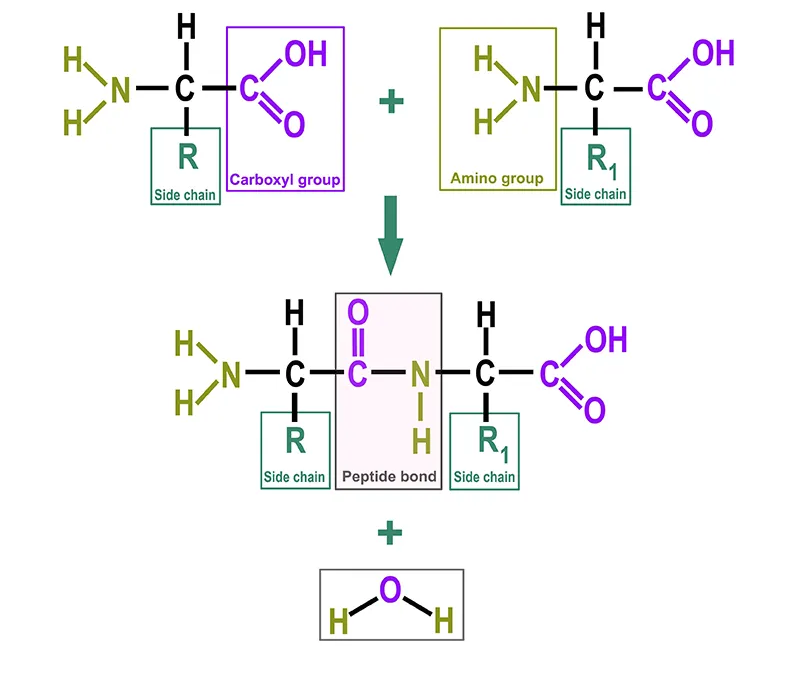
\includegraphics[width=0.4\textwidth]{pics/23_1.png} % INSERIRE QUI LO SCHEMA DELL'AMMINOACIDO
\caption{Struttura generale di un amminoacido. $R$ rappresenta il gruppo residuo (catena laterale).}
\label{fig:ch23_1}
\end{figure}

Dove $R$ è il residuo che definisce il tipo di amminoacido. Esistono 20 tipi comuni di residui, e quindi 20 tipi di amminoacidi.
Gli amminoacidi si legano tra loro attraverso un legame peptidico, che si forma tra il gruppo carbossilico di un amminoacido e il gruppo amminico di un altro, con l'eliminazione di una molecola d'acqua.

Una catena di amminoacidi costituisce la struttura primaria di una proteina. La lunghezza tipica di una proteina è di circa 200 amminoacidi.
Con 20 tipi di amminoacidi e una lunghezza di 200, il numero di sequenze possibili è $20^{200}$, un numero enorme. Tuttavia, solo una frazione molto piccola di queste sequenze possibili corrisponde a proteine funzionali osservate in natura.
Oltre alla sequenza (struttura primaria), sono fondamentali per la funzione di una proteina le sue strutture secondaria, terziaria e quaternaria. Queste descrivono come la catena polipeptidica si ripiega (folds) nello spazio tridimensionale. Le proteine funzionali si trovano tipicamente in una specifica conformazione ripiegata (native state).
Possiamo rappresentare una sequenza proteica come $S = \{S_1, S_2, \dots, S_L\}$, dove $L$ è la lunghezza della proteina ($L \approx 200$) e $S_i \in \{1, \dots, 20\}$ specifica il tipo di amminoacido nella posizione $i$-esima della catena.
La struttura tridimensionale può essere definita specificando le coordinate spaziali di ciascun amminoacido: $\Sigma = \{\vec{r}_1, \vec{r}_2, \dots, \vec{r}_L\}$.

Nel ripiegamento, amminoacidi che sono distanti lungo la catena possono venire a trovarsi vicini nello spazio tridimensionale. Se questi amminoacidi "vicini nello spazio" hanno affinità chimica, possono formare interazioni non covalenti (come legami idrogeno) che stabilizzano la struttura tridimensionale. Questo legame tra sequenza e struttura è cruciale per capire perché solo alcune sequenze sono funzionali.
Le proteine sono spesso divise in famiglie. Proteine appartenenti alla stessa famiglia tendono a ripiegarsi nello stesso modo (stessa struttura tridimensionale) e ad avere funzioni biologiche simili, pur potendo avere sequenze amminoacidiche significativamente diverse (fino al 40\% di differenze). Questo indica che, sebbene la sequenza sia importante, c'è una certa flessibilità.
Per modellizzare una proteina, si può definire un'energia $E(S, \Sigma)$ che dipende sia dalla sequenza $S$ che dalla struttura $\Sigma$. Un'espressione generale per l'energia $E(\{\vec{r}_i\})$ (per una data sequenza $S$) include:

\begin{itemize}
    \item \textbf{Un termine elastico} che mantiene la connettività della catena polipeptidica:
\end{itemize}
\begin{equation} \label{eq:ch23_15}
E_{chain} = \frac{k}{2} \sum_i (\left|\vec{r}_{i+1} - \vec{r}_i\right| - l_0)^2
\end{equation}
dove $l_0$ è la distanza di legame tipica tra amminoacidi adiacenti e $k$ è una costante elastica elevata.

\begin{itemize}
    \item \textbf{Un termine di interazione} tra coppie di amminoacidi $(i,j)$ non necessariamente adiacenti nella sequenza ma che possono trovarsi vicini nello spazio:
\end{itemize}
\begin{equation} \label{eq:ch23_16}
E_{int} = \frac{1}{2} \sum_{i \neq j} V(S_i, S_j) U(\left|\vec{r}_i - \vec{r}_j\right|)
\end{equation}
dove $V(S_i, S_j)$ dipende dal tipo di amminoacidi $S_i$ e $S_j$, e $U(\left|\vec{r}_i - \vec{r}_j\right|)$ è un potenziale che dipende dalla loro distanza.

\begin{itemize}
    \item \textbf{Un termine di volume escluso}, che tiene conto del fatto che due amminoacidi non possono occupare lo stesso spazio. Questo è un termine entropico che può essere rappresentato come un'energia effettiva.
\end{itemize}
\begin{equation} \label{eq:ch23_17}
E_{vol} = \frac{1}{2} \sum_{i \neq j} V_0(\left|\vec{r}_i - \vec{r}_j\right|)
\end{equation}

La forma complessiva dell'energia può essere scritta come:

\begin{equation} \label{eq:ch23_18}
E(\{\vec{r}_i\}) = \frac{k}{2}\sum_{i}(\left|\vec{r}_{i+1}-\vec{r}_i\right|-l_0)^{2} + \frac{1}{2}\sum_{i \neq j}V(S_i,S_j)U(\left|\vec{r}_i-\vec{r}_j\right|) + \frac{1}{2}\sum_{i \neq j}V_0(\left|\vec{r}_i-\vec{r}_j\right|)
\end{equation}

Il paesaggio energetico (energy landscape) di una proteina è fondamentale. Se $V(S_i, S_j)$ fosse una variabile casuale, si otterrebbe un paesaggio energetico simile a quello di un vetro di spin, con molti minimi locali di energia comparabile. Questo non è desiderabile per una proteina, che tipicamente deve raggiungere uno stato nativo ben definito in modo efficiente.
Si pensa che le proteine funzionali abbiano un paesaggio energetico a "imbuto" (funnel), con un minimo globale ben pronunciato che corrisponde allo stato nativo, guidando il ripiegamento verso di esso.


\section{Modello Semplificato}
Per studiare la relazione tra sequenza, struttura ed energia, sono stati proposti modelli semplificati. Uno di questi è il modello HP (Idrofobico-Polare).
\begin{itemize}
    \item La lunghezza della catena è ridotta: $L=27$.
    \item Ci sono solo due tipi di amminoacidi: Idrofobici (H) e Polari (P). Quindi $S_i \in \{H, P\}$.
    \item Gli amminoacidi sono confinati su un reticolo, ad esempio un reticolo cubico 3D. Per $L=27$, la struttura più compatta possibile è un cubo $3 \times 3 \times 3$.
    \item Si definiscono energie di interazione tra amminoacidi adiacenti sul reticolo (non legati covalentemente lungo la catena): $E_{HH}$, $E_{PP}$, $E_{HP}$.
\end{itemize}

Per favorire la formazione di un nucleo idrofobico (con gli amminoacidi H all'interno della proteina, lontani dal solvente acquoso, e i P sulla superficie), si scelgono le energie in modo che l'interazione H-H sia la più favorevole:

\begin{equation} \label{eq:ch23_19}
E_{PP} > E_{HP} > E_{HH} 
\end{equation}

L'energia di una data sequenza $S$ in una data conformazione $\Sigma$ è $E(S, \Sigma)$, data dalla somma delle energie di contatto tra amminoacidi vicini non legati covalentemente.

Studiando lo spazio delle sequenze e delle strutture per questi modelli semplificati, si possono trarre alcune conclusioni:
\begin{itemize}
    \item Non tutte le strutture compatte sono lo stato fondamentale (ground state, GS) di una qualche sequenza. Alcune strutture non sono mai la conformazione di minima energia per nessuna sequenza.
    \item Alcune sequenze hanno uno stato fondamentale degenere, cioè possono ripiegarsi in molte strutture diverse con la stessa energia minima. Questo non è desiderabile per una proteina che deve avere una funzione specifica legata a una struttura specifica.
    \item D'altra parte, la maggior parte delle strutture sono "poco designable": sono lo stato fondamentale di pochissime sequenze. Sarebbe quindi molto improbabile "trovare" una sequenza che si ripiega specificamente in una di queste strutture.
    \item Esiste però un piccolo numero di strutture "altamente designable": sono lo stato fondamentale di un numero molto elevato di sequenze diverse. Queste strutture sono "attrattori" nello spazio delle sequenze.
\end{itemize}

Se si traccia un grafico del numero di strutture che sono il ground state per un dato numero di sequenze, si osserva che un elevato numero di diverse conformazioni strutturali è generato da un esiguo numero di sequenze. Inversamente, solo poche strutture uniche sono associate a un vasto insieme di sequenze. Ciò significa che la maggior parte delle strutture sono "poco designable", mentre poche sono "altamente designable", cioè realizzabili da molte sequenze diverse.
L'idea è che le proteine reali corrispondano a queste strutture altamente designable.

\begin{figure}[h!]
\centering
% 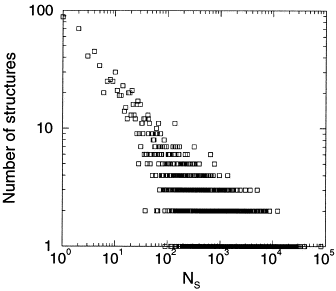
\includegraphics[width=0.6\textwidth]{pics/23_2.png} % INSERIRE QUI IL GRAFICO DELLA DESIGNABILITY
\caption{Grafico della \textit{designability}: sull'asse verticale il numero di strutture differenti, sull'asse orizzontale il numero di sequenze per le quali una data struttura $\Sigma$ rappresenta lo stato di minima energia.}
\label{fig:ch23_2}
\end{figure}

Queste strutture altamente designable spesso presentano particolari simmetrie e sono più stabili. La stabilità è intesa come un ampio gap energetico tra lo stato fondamentale e il primo stato eccitato. Un grande gap significa che la proteina è robusta a piccole perturbazioni e rimane nel suo stato nativo.
Questo approccio aiuta a capire la drastica riduzione dal numero enorme di sequenze possibili al numero relativamente piccolo di strutture proteiche osservate e funzionali.

%-------------------------------------------------------------------------------
% CAPITOLO 24
%-------------------------------------------------------------------------------
\chapter{Lezione 24}
\label{capitolo_24}
\textit{27/05/2026}

\section{Sequenze Proteiche e Modelli di Folding}
Non tutte le sequenze amminoacidiche producono la medesima struttura tridimensionale di una proteina. Ciononostante, si osserva che determinate sequenze, o famiglie di sequenze simili, ricorrono in natura. Questo fenomeno solleva interrogativi sulle proprietà che governano la selezione e la stabilità delle sequenze proteiche funzionali.



Consideriamo una famiglia di proteine:
\begin{itemize}
    \item ciascuna proteina è rappresentata da una sequenza di amminoacidi $\{S_i\}$
    \item una proteina tipica può avere una lunghezza $L=200$ amminoacidi $\longrightarrow i=1, \dots, L$
    \item ci sono 20 possibili amminoacidi $\longrightarrow S_i=1, \dots, 20$
\end{itemize}

Analizziamo l'entropia di queste sequenze per capire la statistica di occorrenza degli amminoacidi.
Il numero totale di sequenze possibili per una proteina di lunghezza $L=200$ è $N_{tot} = 20^{200}$.
L'entropia per una distribuzione di probabilità $P(S)$ su tutte le possibili sequenze è data da:

\begin{equation} \label{eq:ch24_1}
S = -\sum_s P(s) \ln[P(s)]
\end{equation}

dove la somma è su tutte le $20^L$ sequenze.

\subsection*{Assunzione più semplice: indipendenza dei siti}
Assumiamo che la scelta dell'amminoacido in una posizione $i$ sia indipendente dalla scelta degli amminoacidi nelle altre posizioni. La probabilità di una sequenza $S = (S_1, S_2, \dots, S_L)$ è allora il prodotto delle probabilità dei singoli amminoacidi in ciascuna posizione:

\begin{equation} \label{eq:ch24_2}
P(s) = \prod_{i=1}^{L} P^{(i)}(S_i)
\end{equation}

dove $P^{(i)}(S_i)$ è la probabilità che l'amminoacido $S_i$ si trovi in posizione $i$. Questa assunzione potrebbe essere errata.
Sotto questa ipotesi di indipendenza, l'entropia totale diventa additiva:

\begin{align} 
S &= -\sum_{\{S_j\}} \left( \prod_{k=1}^{L} P^{(k)}(S_k) \right) \ln\left[ \prod_{m=1}^{L} P^{(m)}(S_m) \right] \nonumber \\
&= -\sum_{S_1, \dots, S_L} \left( \prod_{k=1}^{L} P^{(k)}(S_k) \right) \sum_{m=1}^{L} \ln[P^{(m)}(S_m)] \nonumber \\
&= -\sum_{m=1}^{200} \Biggl( \sum_{S_m} P^{(m)}(S_m) \ln[P^{(m)}(S_m)] \Biggr) \nonumber \\
&= \sum_{i=1}^{L} S^{(i)} \label{eq:ch24_3}
\end{align}

dove $S^{(i)} = -\sum_{S_i} P^{(i)}(S_i) \ln[P^{(i)}(S_i)]$ è l'entropia associata al sito $i$.
Se non avessimo alcuna informazione, potremmo assumere una probabilità uniforme per ciascun tipo di amminoacido in ogni sito:

\begin{equation} \label{eq:ch24_4}
P^{(i)}(S_i) = \frac{1}{20} \quad \forall i, \forall S_i
\end{equation}

In questo caso, l'entropia per sito sarebbe:

\begin{equation} \label{eq:ch24_5}
S^{(i)} = -\sum_{S_i=1}^{20} \frac{1}{20} \ln\left(\frac{1}{20}\right) = \ln(20)
\end{equation}

E l'entropia totale per una proteina di lunghezza $L=200$ sarebbe:

\begin{equation} \label{eq:ch24_6}
S_{indip,unif} = 200 \ln(20)
\end{equation}

Tuttavia, analizzando un database di $M$ sequenze proteiche allineate, possiamo stimare le frequenze $P^{(i)}(S_i)$ per ogni sito $i$:

\begin{equation} \label{eq:ch24_7}
P^{(i)}(S_i=k) = \frac{n^{(i)}(k)}{M}
\end{equation}

dove $n^{(i)}(k)$ è il numero di volte che l'amminoacido di tipo $k$ appare al sito $i$ nelle $M$ sequenze.
I dati sperimentali ci dicono che non c'è omogeneità: le distribuzioni $P^{(i)}(S_i)$ variano da sito a sito. Quindi, l'assunzione di probabilità uniforme $1/20$ per ogni sito è errata.


\section{Assunzione oltre l'Indipendenza: Correlazioni tra Siti}
Se l'assunzione $P(s) = \prod_i P^{(i)}(S_i)$ non è corretta, dobbiamo considerare le dipendenze tra siti. Un primo passo è introdurre statistiche a due punti (correlazioni tra coppie di siti), come $P(S_i, S_j)$, la probabilità congiunta di osservare l'amminoacido $S_i$ al sito $i$ e l'amminoacido $S_j$ al sito $j$. Questa distribuzione vive in uno spazio di $20 \times 20 = 400$ stati per ogni coppia di siti.



Dai dati, possiamo stimare le correlazioni sperimentali:

\begin{equation} \label{eq:ch24_8}
C_{ij}^{exp} = \langle S_i S_j \rangle_{exp} - \langle S_i \rangle_{exp} \langle S_j \rangle_{exp} 
\end{equation}

L'idea è di costruire un modello probabilistico $P_{mod}(s)$ che riproduca non solo le frequenze dei singoli siti $P^{(i)}(S_i)$ ma anche le correlazioni osservate tra coppie di siti $P(S_i,S_j)$.
Si può usare un algoritmo Monte Carlo per generare un insieme di sequenze artificiali i cui profili di correlazione $C_{ij}^{mod}$ minimizzino la discrepanza con quelli sperimentali $C_{ij}^{exp}$:

\begin{equation} \label{eq:ch24_9}
\chi^2 = \sum_{i,j} |C_{ij}^{mod} - C_{ij}^{exp}|^2
\end{equation}

Studi mostrano che i modelli che includono le interazioni a due punti (correlazioni) sono significativamente migliori nel predire quali sequenze si ripiegano correttamente rispetto ai modelli basati sulla sola statistica dei singoli siti. Questo suggerisce che le interazioni (o co-evoluzioni) tra coppie di amminoacidi lungo la catena sono importanti per il folding. Queste coppie non sono necessariamente adiacenti nella sequenza primaria, ma possono essere in contatto nella struttura tridimensionale ripiegata.


\section{Modello di Massima Entropia (MEM)}
Un approccio formale per costruire modelli probabilistici che siano consistenti con un insieme di osservabili sperimentali è il Modello di Massima Entropia (MEM). Si cerca la distribuzione di probabilità $P(s)$ che massimizza l'entropia $S = -\sum_s P(s) \ln P(s)$ sotto il vincolo che le medie di certe osservabili $O^\mu(s)$ calcolate con $P(s)$ eguaglino i valori sperimentali $\langle O^\mu \rangle_{exp}$:

\begin{equation} \label{eq:ch24_10}
\sum_s P(s) O^\mu(s) = \langle O^\mu \rangle_{exp} \quad \forall \mu
\end{equation}

e la condizione di normalizzazione $\sum_s P(s) = 1$.
La soluzione a questo problema variazionale è una distribuzione della forma:

\begin{equation} \label{eq:ch24_11}
P_{MEM}(s) = \frac{1}{Z} \exp\left(+\sum_\mu \lambda_\mu O^\mu(s)\right)
\end{equation}

dove i $\lambda_\mu$ sono moltiplicatori di Lagrange determinati imponendo i vincoli; la funzione di partizione è data da:

\begin{equation} \label{eq:ch24_12}
Z = \sum_s \exp\left(+\sum_\mu \lambda_\mu O^\mu(s)\right)  
\end{equation}

La massimizzazione dell'entropia vincolata può essere formulata massimizzando il funzionale:

\begin{equation} \label{eq:ch24_13}
\tilde{S}[P, \{\lambda_\mu\}] = -\sum_s P(s) \ln P(s) + \sum_\mu \lambda_\mu \left( \sum_s P(s) O^\mu(s) - \langle O^\mu \rangle_{exp} \right)
\end{equation}

Sostituendo $P_{MEM}(s)$ nel funzionale dell'entropia, si ottiene:

\begin{align} 
\tilde{S}[P, \{\lambda_\mu\}] &= -\sum_s P(s) \Biggl[ -\ln(Z) + \left(\sum_\mu \lambda_\mu O^\mu(s)\right)\Biggr] \nonumber \\
&\quad + \sum_\mu \lambda_\mu \left( \sum_s P(s) O^\mu(s) - \langle O^\mu \rangle_{exp} \right) \label{eq:ch24_14}
\end{align}

Poichè $\sum_s P(s) \ln(Z) = 1 \cdot \ln(Z)$ a causa della normalizzazione, il risultato finale è:

\begin{equation} \label{eq:ch24_15}
\tilde{S}[\{\lambda_\mu\}] = \ln Z[\{\lambda_\mu\}] - \sum_\mu \lambda_\mu \langle O^\mu \rangle_{exp}
\end{equation}

Per determinare i valori ottimali dei $\lambda_\mu$, si pongono a zero le derivate parziali di $\tilde{S}$ rispetto a ciascun $\lambda_\mu$:

\begin{equation} \label{eq:ch24_16}
\frac{\partial\tilde{S}}{\partial\lambda_\mu} = 0
\end{equation}

Consideriamo ora la probabilità di osservare una specifica sequenza sperimentale $S_{exp}$ secondo un modello parametrizzato dai $\lambda_\mu$.

\begin{equation} \label{eq:ch24_17}
P(S_{exp}) = \frac{e^{\sum_\mu \lambda_\mu O^\mu(S_{exp})}}{Z}
\end{equation}

Questa è la probabilità di una singola realizzazione sperimentale $S_{exp}$. Se abbiamo $M$ realizzazioni sperimentali indipendenti $S_{exp}^{(\alpha)}$ (con $\alpha = 1, \dots, M$), indicando l'insieme di queste osservazioni come $\{S_{exp}\}$, la probabilità è:

\begin{equation} \label{eq:ch24_18}
P(\{S_{exp}^{(\alpha)}\}) = \prod_{\alpha=1}^{M} P(S_{exp}^{(\alpha)}) = \prod_{\alpha=1}^{M} \frac{e^{\sum_\mu \lambda_\mu O^\mu(S_{exp}^{(\alpha)})}}{Z}
\end{equation}

Prendendo il logaritmo naturale, si ottiene la Log-Likelihood:

\begin{equation} \label{eq:ch24_19}
\ln P(\{S_{exp}^{(\alpha)}\}) = \sum_{\alpha=1}^{M} \left( -\ln Z + \sum_\mu \lambda_\mu O^\mu(S_{exp}^{(\alpha)}) \right)
\end{equation}

Questa espressione può essere riscritta fattorizzando $M$:

\begin{equation} \label{eq:ch24_20}
\ln P(\{S_{exp}^{(\alpha)}\}) = M \left[ -\ln Z + \frac{1}{M} \sum_{\alpha=1}^{M} \sum_\mu \lambda_\mu O^\mu(S_{exp}^{(\alpha)}) \right]
\end{equation}

Utilizzando la definizione della media sperimentale per ogni osservabile, $\langle O^\mu \rangle_{exp} = \frac{1}{M} \sum_{\alpha=1}^{M} O^\mu(S_{exp}^{(\alpha)})$, la Log-Likelihood diventa:

\begin{equation} \label{eq:ch24_21}
\ln P(\{S_{exp}^{(\alpha)}\}) = M \left( -\ln Z + \sum_\mu \lambda_\mu \langle O^\mu \rangle_{exp} \right)
\end{equation}

Massimizzare questa Log-Likelihood rispetto ai $\lambda_\mu$ è equivalente a risolvere il sistema di equazioni $\langle O^\mu \rangle_{model} = \langle O^\mu \rangle_{exp}$.

%-------------------------------------------------------------------------------
% CAPITOLO 25
%-------------------------------------------------------------------------------
\chapter{Lezione 25}
\label{capitolo_25}
\textit{30/05/2025}

\section{Modelli Generativi per l'Evoluzione e la Progettazione delle Proteine}
Lo studio delle proteine attraverso modelli statistici si prefigge come obiettivo primario la comprensione della loro struttura tridimensionale e della loro funzione biologica partendo dalla semplice sequenza amminoacidica. Le proteine, polimeri costituiti da amminoacidi, sono rappresentabili come stringhe di lettere, dove ogni lettera corrisponde a uno dei 20 amminoacidi naturali, a cui si può aggiungere un simbolo per eventuali "gap" negli allineamenti.

Il percorso che lega la sequenza alla funzione può essere semplificato nel dogma:
\textbf{Sequenza $\rightarrow$ Struttura $\rightarrow$ Funzione}

La prima transizione, da sequenza a struttura, è oggi considerata un problema in gran parte risolto, grazie soprattutto a strumenti come AlphaFold. In questo caso, si passa da un oggetto unidimensionale (la stringa di amminoacidi) a un oggetto matematico ben definito nello spazio tridimensionale (le coordinate degli atomi). La disponibilità di vasti dataset ha giocato un ruolo cruciale in questo progresso.

Tuttavia, il passaggio successivo, dalla struttura alla funzione, o direttamente dalla sequenza alla funzione, si rivela molto più arduo e costituisce un campo di ricerca ancora ampiamente aperto. Le difficoltà principali risiedono nella natura stessa della "funzione", un concetto spesso mal definito e che comprende molteplici aspetti. Inoltre, la funzione è fortemente dipendente dal contesto e dall'ambiente cellulare, e la sua misurazione sperimentale quantitativa è intrinsecamente complessa, portando a una scarsità di dati rispetto a quelli strutturali.

Le applicazioni che deriverebbero da una piena comprensione di questi legami sono molteplici: la progettazione di proteine artificiali con funzionalità specifiche, la comprensione dei meccanismi dell'evoluzione naturale e l'ottimizzazione dei protocolli di evoluzione diretta condotta in laboratorio.

Ci sono diverse tipologie di dati sperimentali:

\begin{itemize}
    \item \textbf{Sequenze naturali e MSA:} Una fonte primaria è costituita dalle sequenze di proteine naturali, ottenute tramite Allineamenti Multipli di Sequenze (MSA). Queste sequenze sono il frutto dell'evoluzione naturale; specie diverse spesso possiedono versioni omologhe della stessa proteina che, pur differendo nella sequenza, mantengono struttura e funzione simili. Un esempio emblematico è la beta-lattamasi, un enzima coinvolto nella resistenza agli antibiotici, di cui si conoscono circa 5000 varianti naturali che possono presentare anche solo il 20-30\% di identità di sequenza tra loro. Database pubblici come UniProt raccolgono queste informazioni. L'analisi statistica degli MSA si concentra principalmente su due aspetti: la \textit{conservazione}, ovvero la frequenza di ciascun amminoacido in ogni posizione dell'allineamento, che evidenzia siti cruciali per la struttura o la funzione; e la \textit{coevoluzione}, che studia le correlazioni tra amminoacidi in posizioni diverse, indicative di possibili contatti fisici nella struttura 3D.
    \item \textbf{Deep Mutational Scans (DMS):} In questi esperimenti, si parte da una sequenza proteica naturale e si introducono sistematicamente tutte le possibili mutazioni puntiformi (= cambiamento di un singolo amminoacido) in ciascuna posizione. Successivamente, si misura l'effetto di ogni mutazione sulla funzione della proteina, ad esempio valutando la sopravvivenza di batteri che la esprimono in presenza di un antibiotico. I DMS forniscono quindi informazioni dettagliate sullo "spazio funzionale" locale attorno a una specifica sequenza. Il numero di esperimenti di questo tipo è in costante crescita e permette anche di confrontare l'effetto di una mutazione in contesti genetici differenti.
    \item \textbf{Evoluzione in vitro:} Mirano a mimare il processo evolutivo naturale, ma in condizioni rigorosamente controllate. Il processo tipico prevede di partire da una sequenza wild-type, generare una libreria di mutanti (ad esempio tramite PCR), applicare una pressione selettiva (come un antibiotico), selezionare i mutanti che mostrano un fenotipo "migliore" (es. sopravvivenza) e iterare questo ciclo. Questi esperimenti producono librerie di sequenze che presentano un numero limitato di mutazioni rispetto alla sequenza iniziale (ad esempio, 20-50 mutazioni dopo centinaia di generazioni), ma il vantaggio risiede nel poter analizzare un gran numero di sequenze per ogni generazione grazie alle moderne ed economiche tecniche di sequenziamento. I principali vantaggi sono il controllo delle condizioni sperimentali e la tracciabilità del percorso evolutivo.
    \item \textbf{Ricostruzioni filogenetiche:} Partendo dalle sequenze di proteine moderne, si possono inferire le sequenze di proteine che esistevano in organismi ancestrali. Queste proteine "ancestrali" possono poi essere sintetizzate e caratterizzate in laboratorio per studiarne le proprietà, permettendo di esplorare i cammini evolutivi che hanno mantenuto la funzione attraverso lo spazio delle sequenze. Un esempio illustrativo è lo studio di due proteine fluorescenti con la stessa struttura ma colori di emissione diversi (blu vs. rosso), separate da 13 mutazioni: testando tutti i $2^{13}$ intermedi si è potuto osservare un "collo di bottiglia" funzionale nel passaggio da una funzione all'altra.
\end{itemize}


\section{Dalla sequenza alla struttura}
Un'applicazione fondamentale dell'analisi degli MSA è la predizione dei contatti tra residui amminoacidici nella struttura tridimensionale della proteina. L'input è un allineamento multiplo (es. inibitore della tripsina = una proteina di 53 siti, con circa 13600 sequenze allineate), e l'output desiderato è identificare quali coppie di siti si trovano spazialmente vicine. Convenzionalmente, due residui sono considerati in contatto se la distanza tra i loro atomi è inferiore a una certa soglia, tipicamente intorno agli $8 \text{ \AA}$.

L'analisi statistica dell'MSA inizia con una rappresentazione numerica delle sequenze. Ogni sito della sequenza viene trasformato in un vettore binario di lunghezza 20 (o 21, includendo il gap), dove una singola posizione del vettore è 1 e le altre 0. Ad esempio, il gap potrebbe essere $[1,0,\dots,0]$, l'alanina (A) $[0,1,\dots,0]$, la cisteina (C) $[0,0,1,\dots,0]$, e così via, con l'ultimo amminoacido rappresentato da un vettore di tutti zeri per evitare problemi di collinearità. L'intero MSA si trasforma così in una grande matrice numerica.

Da questa matrice si possono calcolare le frequenze di singolo sito, $P_i(a)$, che indicano la frequenza dell'amminoacido $a$ al sito $i$ e riflettono la conservazione di quella posizione. Queste si ottengono semplicemente sommando i vettori per ogni colonna corrispondente a un amminoacido in una data posizione e normalizzando per il numero totale di sequenze.
Analogamente, si calcolano le frequenze di coppie di siti, $P_{ij}(a,b)$, che rappresentano la frequenza con cui l'amminoacido $a$ si trova al sito $i$ contemporaneamente all'amminoacido $b$ al sito $j$ nella stessa sequenza. Queste possono essere stimate tramite il prodotto $(X^T X) / M$, dove $X$ è la matrice binaria e $M$ il numero di sequenze. Da queste frequenze si deriva la matrice di covarianza:

\begin{equation} \label{eq:ch25_1}
C_{ij}(a,b) = P_{ij}(a,b) - P_i(a)P_j(b)
\end{equation}

che misura quanto la co-occorrenza di due amminoacidi devia dall'indipendenza statistica.

Un primo approccio per identificare i contatti si basa sulla \textbf{Mutua Informazione (MI)}. Questa grandezza misura la dipendenza statistica tra due siti $i$ e $j$, mediando su tutte le possibili coppie di amminoacidi:

\begin{equation} \label{eq:ch25_2}
MI(i,j) = \sum_{a,b} P_{ij}(a,b) \log \frac{P_{ij}(a,b)}{P_i(a)P_j(b)}
\end{equation}

La MI è sempre non negativa e si annulla se e solo se i due siti sono statisticamente indipendenti.
L'ipotesi sottostante è che coppie di siti con un'alta MI siano probabilmente a contatto nella struttura. La procedura consiste nel calcolare la MI per tutte le coppie di siti, ordinarle in base a questo valore e considerare le coppie al vertice della lista come predizioni di contatto.
Sebbene questo metodo funzioni bene per le primissime predizioni (prime 10), la sua precisione tende a diminuire rapidamente all'aumentare del numero di contatti predetti, generando molti falsi positivi.
Per mitigare questo problema, sono state proposte correzioni empiriche come l'APC (Average Product Correction), che tentano di ridurre l'effetto di correlazioni spurie. Questi metodi, tuttavia, portano a miglioramenti generalmente modesti.

Una nota tecnica importante riguarda l'uso di \textit{pseudocounts}: si tratta di aggiungere un piccolo valore (un prior) alle frequenze osservate per evitare che il campionamento finito porti a frequenze nulle, specialmente per eventi rari, migliorando così la robustezza delle stime di probabilità.


\section{Analisi degli Accoppiamenti Diretti}
Il limite principale della Mutua Informazione risiede nel fatto che la correlazione non implica causalità. Se un sito A è a contatto con B, e B è a contatto con C, A e C potrebbero apparire statisticamente correlate anche in assenza di un contatto diretto tra loro.
L'Analisi degli Accoppiamenti Diretti (DCA, Direct Coupling Analysis) si propone di superare questa limitazione, distinguendo le interazioni dirette da quelle indirette.

Per formalizzare questo approccio, si considera un modello probabilistico per le variabili $y_1, \dots, y_n$ dove $y_{ia} = (\sigma_{ia} - P_{ia})/P_{ia}$. Si assume che la probabilità congiunta di osservare una particolare configurazione di queste variabili sia data da una distribuzione di tipo:

\begin{equation} \label{eq:ch25_3}
P(y_1, \dots, y_n) \propto \exp\left(-\frac{1}{2} \sum_{i,j} y_i J_{ij} y_j\right)
\end{equation}

In questo modello, i coefficienti $J_{ij}$ rappresentano le interazioni o accoppiamenti diretti tra la variabile $i$ e la variabile $j$. Se $J_{ij}=0$, allora la variabile $i$ non interagisce direttamente con la variabile $j$ (anche se potrebbero comunque risultare correlate a causa di interazioni mediate da altre variabili).
La probabilità condizionale di $y_i$, dati i valori di tutte le altre variabili $y_{k \neq i}$, dipende solo dagli accoppiamenti $J_{ij}$ che coinvolgono $y_i$: 

\begin{equation} \label{eq:ch25_4}
P(y_i | y_{k \neq i}) \propto \exp\left(-\frac{1}{2} y_i \sum_j J_{ij} y_j\right)
\end{equation}

L'obiettivo diventa quindi dedurre i parametri di accoppiamento $J_{ij}$ a partire dalla matrice di covarianza $C$ osservata dai dati. Ciò può essere fatto con diverse approssimazioni:

\begin{itemize}
    \item \textbf{Approssimazione Gaussiana:} Se si assume che le variabili $y_i$ seguano una distribuzione Gaussiana multivariata, allora la relazione tra la matrice di covarianza $C$ e la matrice di accoppiamento $J$ è esatta:
    \begin{equation} \label{eq:ch25_5}
    C = J^{-1}
    \end{equation}
    Sebbene le nostre variabili (che rappresentano la presenza/assenza di un tipo di amminoacido in un sito, quindi binarie 0/1) non siano intrinsecamente Gaussiane, questa approssimazione può comunque essere applicata come metodo pratico.
    
    \item \textbf{Approssimazione di Campo Medio:} Questa approssimazione è più adatta per variabili binarie. Si assume che il valore medio di una variabile $y_i$ sia dato da una funzione non lineare $F$ (come una tangente iperbolica per spin $\pm 1$) del campo medio che agisce su di essa:
    \begin{equation} \label{eq:ch25_6}
    \langle y_i \rangle = \left\langle F\left[h_i + \sum_j J_{ij} y_j\right] \right\rangle \approx F\left[h_i + \sum_j J_{ij} \langle y_j \rangle\right]
    \end{equation}
    dove $h_i$ sono campi locali. Utilizzando il Teorema Fluttuazione-Dissipazione (FDT), che lega la matrice di covarianza $C_{ik}$ alla derivata del valor medio $\langle y_i \rangle$ rispetto a un campo locale fittizio $h_k$:
    \begin{equation} \label{eq:ch25_7}
    C_{ik} = \frac{\partial \langle y_i \rangle }{ \partial h_k}\bigg|_{h=0}
    \end{equation}
    si può derivare una relazione approssimata tra $C$ e $J$.
\end{itemize}

Questa relazione, in forma matriciale, è $C = D[I+JC]$ (dove $I$ è la matrice identità e $D$ è una matrice diagonale i cui elementi $D_{ii}$ dipendono dalla derivata $F'$ della funzione non lineare, calcolata nel punto di campo medio). Risolvendo per $J$, si ottiene:

\begin{equation} \label{eq:ch25_8}
J = D^{-1} - C^{-1}
\end{equation}

Se si è interessati solo ai termini fuori diagonale (che rappresentano le interazioni tra siti diversi), il termine diagonale $D^{-1}$ può essere ignorato, e si considera $J \approx -C^{-1}$ (il segno dipende dalle convenzioni).

Una volta ricavati gli accoppiamenti diretti $J_{ij}(a,b)$, per ottenere un singolo punteggio di accoppiamento per ogni coppia di siti $(i,j)$, si aggregano questi valori calcolando la norma di Frobenius $F_{ij} = \sum_{a,b} (J_{ij}(a,b))^2$ su tutti i possibili amminoacidi $a$ e $b$.
Infine, le coppie di siti $(i,j)$ vengono ordinate in base a questi punteggi $F_{ij}$ decrescenti. Questo approccio ha dimostrato un significativo miglioramento nella predizione dei contatti rispetto alla MI, fornendo un numero maggiore di predizioni corrette.
La rilevanza del DCA è sottolineata dal fatto che questo metodo costituisce un componente chiave dell'algoritmo AlphaFold.

\textbf{Connessione di questi metodi con il modello di Ising:}
\begin{itemize}
    \item La relazione tra correlazione e funzione di risposta (FDT) è usata qui in modo inverso rispetto a come si fa solitamente per il modello di Ising standard. In quel caso, si conoscono le interazioni $J_{ij}$ (es. tra primi vicini su un reticolo) e si vuole calcolare la matrice di correlazione $C_{ij}$; qui, invece, si misura $C_{ij}$ dai dati di sequenza e si vuole inferire la matrice di accoppiamento $J_{ij}$.
    \item La distribuzione di probabilità $P(y_1, \dots, y_n) \propto \exp(-\frac{1}{2} \sum y_i J_{ij} y_j)$ che viene utilizzata in questi metodi è esattamente la distribuzione che si otterrebbe applicando un approccio di Massima Entropia, se si richiedesse al modello di riprodurre esattamente le correlazioni a uno e due punti misurate dai dati sperimentali.
\end{itemize}


\section{Modelli Generativi per Proteine}
Oltre alla predizione strutturale, un obiettivo è la generazione di nuove sequenze proteiche che siano funzionali. Questo si inserisce nel campo dei modelli generativi, con analogie ai modelli per la generazione di immagini o di testo (come ChatGPT e altri).
Tuttavia, un approccio alternativo, basato sulla fisica statistica e sul principio di Massima Entropia, offre alcuni vantaggi, specialmente quando si lavora con quantità di dati che, sebbene grandi, sono comunque inferiori a quelle usate per addestrare i grandi modelli linguistici. Questo approccio si propone di costruire modelli più semplici e interpretabili rispetto alle complesse "black box" delle reti neurali profonde.

L'applicazione del principio di Massima Entropia porta naturalmente alla seguente distribuzione di probabilità:

\begin{equation} \label{eq:ch25_9}
P(a_1, \dots, a_L) = \frac{1}{Z} \exp\left(\sum_i h_i(a_i) + \sum_{i<j} J_{ij}(a_i, a_j)\right) = \frac{1}{Z} e^{-E(a_1,\dots,a_L)}
\end{equation}

In questa espressione, $h_i(a_i)$ sono responsabili di riprodurre le frequenze di conservazione $P_{ia}$ osservate. $J_{ij}(a_i, a_j)$ sono responsabili di riprodurre le frequenze di coevoluzione $P_{ia,jb}$ osservate.
In questo caso l'approssimazione di campo medio si rivela non sufficientemente accurata, bisogna trovare i valori esatti di $h_i$ e $J_{ij}$ che meglio si adattano ai dati. L'algoritmo comunemente usato per questo scopo è il \textbf{Boltzmann Learning}.

L'idea di base è la seguente:
\begin{enumerate}
    \item Si parte da un insieme di dati da cui si misurano le frequenze di singolo sito $P_{ia}^{data}$ e le frequenze di coppia $P_{ia,jb}^{data}$.
    \item Si inizializzano i parametri del modello $h_i$ e $J_{ij}$.
    \item Dal modello corrente, si calcolano le statistiche predette dal modello: $P_{ia}^{model}$ e $P_{ia,jb}^{model}$. Per calcolare queste medie nel modello, si ricorre a tecniche di campionamento Monte Carlo.
    \item Si confrontano le statistiche del modello con quelle dei dati. Se non coincidono, si aggiornano i parametri $h_i$ e $J_{ij}$ in una direzione che riduca la discrepanza. Si itera questo processo finché le statistiche del modello non si avvicinano sufficientemente a quelle dei dati.
\end{enumerate}


%-------------------------------------------------------------------------------
% CAPITOLO 26
%-------------------------------------------------------------------------------
\chapter{Lezione 26}
\label{capitolo_26}
\textit{03/06/2025}


\section{Introduzione alla Materia Attiva}

Si definisce \textbf{materia attiva} l'insieme di tutti quei sistemi i cui costituenti individuali sono "attivi", ovvero possiedono un qualche meccanismo (interno o esterno) che funge da motore. Un esempio classico è un batterio, che è un oggetto attivo: possiede flagelli e un meccanismo che trasforma i nutrienti in movimento (il motore molecolare). Molti altri sistemi, sia viventi che non, sono costituiti da particelle auto-propellenti.

Il meccanismo di auto-propulsione è dovuto a una forza che non specificheremo in dettaglio, il cui effetto è quello di permettere alla particella di muoversi anche in assenza di forze esterne.

I batteri sono particolarmente interessanti perché operano alla stessa scala di grandezza del moto Browniano. Per comprendere la novità introdotta dalla materia attiva, è utile richiamare il modello del moto Browniano passivo.

\subsection{Richiamo: Moto Browniano Passivo}
Il moto Browniano è causato dagli urti casuali delle molecole del solvente (es. acqua) su una particella. Tramite questi urti, le particelle Browniane scambiano energia e momento con il bagno termico. Il moto di una particella Browniana in un potenziale esterno $\vec{F}(\vec{x})$ è descritto dall'equazione di Langevin:
\begin{equation}
    m\frac{d^{2}\vec{x}}{dt^{2}} + \zeta\frac{d\vec{x}}{dt} = \vec{F}(\vec{x}) + \delta\vec{F}(t)
\end{equation}


Il termine $\delta\vec{F}(t)$ rappresenta una forza stocastica (rumore bianco) con le seguenti proprietà:
\begin{equation}
    \langle \delta F_{\alpha}(t) \rangle = 0 \quad \forall \alpha, t
\end{equation}
\begin{equation}
    \langle \delta F_{\alpha}(t) \delta F_{\beta}(t') \rangle = 2k_{B}T\zeta \, \delta(t-t') \delta_{\alpha\beta} \label{eq:fluct-dissip}
\end{equation}
dove $\alpha, \beta \in \{x, y, z\}$. La presenza della temperatura $T$ in questa relazione (relazione di fluttuazione-dissipazione di Einstein) è fondamentale, poiché indica che il rumore è di origine termica.

In un sistema del genere, all'equilibrio, valgono i principi della meccanica statistica. Ad esempio, per una particella in un potenziale armonico $V(x) = \frac{1}{2}kx^2$ (corrispondente a una forza $F(x) = -kx = -\frac{dV}{dx}$) , la distribuzione di probabilità stazionaria è quella di Gibbs-Boltzmann , e la distribuzione delle velocità segue la statistica di Maxwell-Boltzmann:
\begin{equation}
    P(\vec{v}) \propto e^{-\frac{\beta m v^2}{2}} \quad \text{con} \quad \beta = \frac{1}{k_B T}
\end{equation}

\subsection{Caratteristiche dei Sistemi Attivi}
A differenza dei sistemi passivi, dove l'energia viene fornita "dall'esterno" (ad esempio, tramite uno stress applicato ai bordi di un fluido per metterlo in moto) , nei sistemi attivi l'energia viene iniettata a livello del singolo individuo. Il "motore" è un meccanismo che permette all'individuo di regolare la propria velocità , in modo diverso da come il bagno termico impone la distribuzione di Maxwell-Boltzmann alle particelle passive.

Pensiamo a un'automobile: si immette carburante (energia) che permette di regolare la velocità agendo sull'acceleratore. Analogamente, un sistema attivo sfrutta una qualche forma di energia interna per regolare la sua velocità. Ad esempio, il batterio \textit{E. coli} idrolizza ATP per alimentare il suo motore flagellare, potendo così impostare una velocità diversa da quella che avrebbe a causa del solo moto Browniano.

Tipicamente, la forza interna che porta il sistema fuori dall'equilibrio non è nota in dettaglio. In uno stormo di uccelli, ad esempio, è impossibile monitorare lo stato fisiologico di ogni singolo uccello per prevedere le variazioni della sua velocità.

\section{Modello della Particella Attiva Browniana (ABP)}
Per modellare questi sistemi, partiamo dall'equazione di Langevin di secondo ordine e la riscriviamo come un sistema di due equazioni del primo ordine:
\begin{equation}
    \begin{cases}
        \frac{d\vec{x}}{dt} = \vec{v} \\
        m\frac{d\vec{v}}{dt} = -\zeta\vec{v} + \vec{F}(\vec{x}) + \delta\vec{F}(t)
    \end{cases}
\end{equation}
Dividendo la seconda equazione per la massa $m$ otteniamo:
\begin{equation}
    \frac{d\vec{v}}{dt} = -\frac{\zeta}{m}\vec{v} + \frac{\vec{F}(\vec{x})}{m} + \frac{\delta\vec{F}(t)}{m} = -\gamma\vec{v} + \vec{F}'(\vec{x}) + \vec{\xi}(t) \label{eq:langevin_vel}
\end{equation}
dove $\gamma = \zeta/m$ è il coefficiente di frizione, $\vec{F}' = \vec{F}/m$ è la forza per unità di massa e $\vec{\xi} = \delta\vec{F}/m$ è il rumore per unità di massa.

La differenza cruciale per una particella \textbf{attiva} è che il termine di attrito non è costante, ma dipende dalla velocità della particella:
\begin{equation}
    \gamma \rightarrow \gamma(|\vec{v}|)
\end{equation}
L'equazione (\ref{eq:langevin_vel}) diventa:
\begin{equation}
    \frac{d\vec{v}}{dt} = -\gamma(|\vec{v}|)\vec{v} + \vec{F}'(\vec{x}) + \vec{\xi}(t)
\end{equation}
Questo termine dipendente dalla velocità può essere interpretato in due modi:
\begin{itemize}
    \item Come una \textbf{viscosità dipendente dalla velocità}.
    \item Come una \textbf{forza attiva} $\vec{F}_{act}(\vec{v})$ che regola la velocità.
\end{itemize}
Per i sistemi che studieremo, la seconda interpretazione è più significativa. Riscriviamo quindi il termine come $\vec{F}_{act}(\vec{v})$. \textit{(Nota: questa forza ha le dimensioni di un'accelerazione, avendo diviso per la massa, ma è solo un cambio di unità di misura).}

Il sistema di equazioni per una particella attiva diventa:
\begin{equation}
    \begin{cases}
        \frac{d\vec{x}}{dt} = \vec{v} \\
        \frac{d\vec{v}}{dt} = \vec{F}_{act}(\vec{v}) + \vec{F}(\vec{x}) + \vec{\xi}(t)
    \end{cases}
    \label{eq:sistema_attivo}
\end{equation}
\textit{(D'ora in poi, per semplicità, omettiamo l'apice sulla forza $\vec{F}(\vec{x})$ ).}

Assumiamo che la forza attiva derivi da un potenziale che dipende dalla velocità:
\begin{equation}
    \vec{F}_{act}(\vec{v}) = -\frac{\partial}{\partial\vec{v}} \Phi_{act}(\vec{v})
\end{equation}
Questa assunzione è analoga a quella di avere forze conservative derivanti da un potenziale dipendente dalla posizione. Il potenziale $\Phi_{act}(\vec{v})$ modella i vincoli fisiologici o meccanici che definiscono una velocità tipica per l'individuo (es. uno storno non può volare alla velocità del suono).

\section{Dall'Equazione di Langevin all'Equazione di Fokker-Planck}

Se una variabile stocastica $x(t)$ obbedisce a un'equazione di Langevin, la sua distribuzione di probabilità $P(x, t)$ evolve secondo un'equazione di Fokker-Planck. Per il caso sovrasmorzato (\textit{overdamped}) in una dimensione, l'equazione di Langevin è:
\begin{equation}
    \frac{dx}{dt} = \frac{F(x)}{\zeta} + \xi(t)
\end{equation}
e la corrispondente equazione di Fokker-Planck è:
\begin{equation}
    \frac{\partial P}{\partial t} = D \frac{\partial^2 P}{\partial x^2} - \frac{\partial}{\partial x}\left[ \frac{F(x)P}{\zeta} \right] = -\frac{\partial J}{\partial x}
\end{equation}
dove $D$ è il coefficiente di diffusione e $J$ è la corrente di probabilità.

Il nostro obiettivo è trovare l'equazione di Fokker-Planck per il sistema generale attivo descritto da (\ref{eq:sistema_attivo}). Per farlo, useremo una tecnica che riscrive il sistema di equazioni come una singola equazione di Langevin sovrasmorzata in uno spazio a dimensioni maggiori.

\subsection{Formalismo dei Super-Vettori}
Introduciamo dei "super-vettori" che vivono in uno spazio a $2d$ dimensioni (se la particella si muove in $d$ dimensioni):
\begin{equation}
    \underline{w} = \begin{pmatrix} \vec{x} \\ \vec{v} \end{pmatrix}, \quad
    \underline{\mathcal{F}}(\underline{w}) = \begin{pmatrix} \vec{v} \\ \vec{F}(\vec{x}) + \vec{F}_{act}(\vec{v}) \end{pmatrix}, \quad
    \underline{\eta}(t) = \begin{pmatrix} \vec{0} \\ \vec{\xi}(t) \end{pmatrix}
\end{equation}


Con questa notazione, il sistema (\ref{eq:sistema_attivo}) diventa una singola equazione di Langevin di tipo sovrasmorzato per il super-vettore $\underline{w}$:
\begin{equation}
    \frac{d\underline{w}}{dt} = \underline{\mathcal{F}}(\underline{w}) + \underline{\eta}(t) \label{eq:super_langevin}
\end{equation}
Scrivendo questa equazione componente per componente (dove una componente è un vettore $d$-dimensionale), si riottiene il sistema di partenza.

Poiché l'equazione (\ref{eq:super_langevin}) ha la forma di un'equazione di Langevin sovrasmorzata, possiamo scrivere direttamente la corrispondente equazione di Fokker-Planck. La distribuzione di probabilità dipenderà ora dal super-vettore: $P(\underline{w}, t) = P(\vec{x}, \vec{v}, t)$.

L'equazione di Fokker-Planck generale (detta "Super Fokker-Planck") è:
\begin{equation}
    \frac{\partial P}{\partial t} = - \frac{\partial}{\partial \underline{w}} \cdot \underline{\vec{J}} = - \frac{\partial}{\partial \underline{w}} \cdot \left[ \underline{\mathcal{F}} P - \mathbf{B} \frac{\partial P}{\partial \underline{w}} \right]
    \label{eq:super_FP}
\end{equation}
Il termine $\mathbf{B}$ è una "matrice di diffusione". Le sue componenti $B_{\alpha\beta}$ sono legate al correlatore del super-rumore $\underline{\eta}$. Dato che il rumore $\vec{\xi}(t)$ agisce solo sulla velocità , la matrice $\mathbf{B}$ ha una forma a blocchi:
\begin{equation}
    \mathbf{B} = 
    \begin{pmatrix}
        \mathbf{0}_{d \times d} & \mathbf{0}_{d \times d} \\
        \mathbf{0}_{d \times d} & B \cdot \mathbf{I}_{d \times d}
    \end{pmatrix}
\end{equation}
dove $B$ è una costante di diffusione legata all'intensità del rumore: \\ $\langle \xi_\alpha(t)\xi_\beta(t') \rangle = 2B \delta_{\alpha\beta}\delta(t-t')$. 

\subsection{Equazione di Fokker-Planck Esplicita per Particelle Attive}
Esplicitando i termini nell'equazione (\ref{eq:super_FP}) e usando la forma di $\underline{w}$, $\underline{\mathcal{F}}$ e $\mathbf{B}$, si ottiene l'equazione di Fokker-Planck per particelle attive:
\begin{equation}
    \frac{\partial P}{\partial t} = B \frac{\partial^2 P}{\partial \vec{v}^2} - \vec{v} \cdot \frac{\partial P}{\partial \vec{x}} - \vec{F}(\vec{x}) \cdot \frac{\partial P}{\partial \vec{v}} - \frac{\partial}{\partial \vec{v}} \cdot \left( \vec{F}_{act}(\vec{v}) P \right)
    \label{eq:FP_attiva}
\end{equation}
dove $P = P(\vec{x}, \vec{v}, t)$.

\section{Analisi di Casi Specifici}

\subsection{Caso Passivo ($F_{act} = -\gamma \vec{v}$)}
Consideriamo una particella passiva, dove la "forza attiva" è semplicemente l'attrito viscoso lineare: $\vec{F}_{act}(\vec{v}) = -\gamma \vec{v}$. Questo corrisponde a un potenziale di velocità armonico: $\Phi_{act}(\vec{v}) = \frac{1}{2}\gamma v^2$. In questo caso, la distribuzione stazionaria ($\partial P / \partial t = 0$) è la ben nota distribuzione di Gibbs-Boltzmann per l'Hamiltoniana classica $H(\vec{x}, \vec{v}) = V(\vec{x}) + \frac{1}{2}mv^2$:
\begin{equation}
    P_{st}(\vec{x}, \vec{v}) = \frac{e^{-\beta H(\vec{x}, \vec{v})}}{Z}
\end{equation}
Questo conferma che il formalismo generale recupera i risultati noti della meccanica statistica all'equilibrio.

\subsection{Caso Attivo in Assenza di Forze Esterne ($\vec{F}(\vec{x}) = \vec{0}$)}
Consideriamo ora una particella attiva senza forze esterne , quindi senza posizioni privilegiate nello spazio. Per tempi molto lunghi, ci aspettiamo che la distribuzione di probabilità diventi uniforme nello spazio, ovvero non dipenda da $\vec{x}$:
\begin{equation}
    P_{st}(\vec{x}, \vec{v}) = \text{costante} \times P(\vec{v}) \implies \frac{\partial P}{\partial \vec{x}} = \vec{0}
    \label{eq:ansatz_homog}
\end{equation}
Sostituendo questa forma nell'equazione di Fokker-Planck (\ref{eq:FP_attiva}) e ponendo $\vec{F}(\vec{x})=\vec{0}$ e $\partial P / \partial t = 0$, i termini dipendenti da $\vec{x}$ si annullano e otteniamo un'equazione per la sola distribuzione delle velocità $P(\vec{v})$:
\begin{equation}
    B \frac{\partial^2 P}{\partial \vec{v}^2} - \frac{\partial}{\partial \vec{v}} \cdot \left( \vec{F}_{act}(\vec{v}) P \right) = 0
\end{equation}
Questa è un'equazione di Fokker-Planck stazionaria per la variabile $\vec{v}$, la cui soluzione è una distribuzione canonica nella velocità:
\begin{equation}
    P_{st}(\vec{v}) = \frac{e^{-\Phi_{act}(\vec{v})/B}}{Z_v}
    \label{eq:distr_vel_attiva}
\end{equation}
dove $Z_v$ è la costante di normalizzazione. Questo risultato è fondamentale: il potenziale attivo $\Phi_{act}$ permette di "ingegnerizzare" la distribuzione delle velocità, a differenza del caso passivo dove è sempre una Maxwelliana.

\subsubsection{Esempio: Potenziale a "Cappello Messicano"}
Consideriamo un potenziale attivo della forma:
\begin{equation}
    \Phi_{act}(\vec{v}) = -\left( \frac{a}{2}v^2 - \frac{b}{4}v^4 \right) \quad \text{con } a, b > 0
\end{equation}
Questa è una funzione radiale (dipende solo dal modulo $v=|\vec{v}|$). Per trovare la velocità più probabile, cerchiamo i minimi del potenziale (o i massimi dell'esponenziale in (\ref{eq:distr_vel_attiva})). La derivata rispetto a $v$ è:
\begin{equation}
    \frac{\partial \Phi_{act}}{\partial v} = -av + bv^3 = v(bv^2 - a)
\end{equation}
Annullando la derivata troviamo un massimo locale in $v=0$ e un minimo per:
\begin{equation}
    v_0 = \sqrt{\frac{a}{b}}
\end{equation}
In 2D, questo potenziale ha la forma di un "cappello messicano" (o \textit{double well} in sezione), con un anello di minimo a raggio $v_0$. La distribuzione di probabilità $P_{st}(\vec{v})$ sarà quindi massima per tutte le velocità $\vec{v}$ tali che $|\vec{v}|=v_0$.

\subsection{Limite a Velocità Costante}
Consideriamo il limite in cui la barriera di potenziale diventa infinitamente alta, ovvero $a/B \to \infty$ e $b/B \to \infty$, mantenendo il rapporto $v_0 = \sqrt{a/b}$ finito. In questo limite, l'approssimazione di discesa più ripida (\textit{steepest descent}) implica che solo gli stati sul minimo del potenziale (massimo della probabilità) contribuiscono. La distribuzione di probabilità diventa:
\begin{equation}
    P_{st}(\vec{v}) \propto \delta(|\vec{v}| - v_0)
\end{equation}
Questo descrive un sistema di particelle che si muovono tutte con \textbf{velocità di modulo costante} $v_0$, ma la cui direzione $\theta$ può fluttuare liberamente.

\subsubsection{Algoritmi di Simulazione}
Questo sistema limite può essere simulato in due modi principali:
\begin{enumerate}
    \item \textbf{Riorientamento continuo:} Il modulo della velocità è fisso a $v_0$. L'angolo $\theta$ della velocità evolve secondo un'equazione di Langevin per la sola variabile angolare:
    \begin{equation}
        \frac{d\theta}{dt} = \xi(t)
    \end{equation}
    dove $\xi(t)$ è un rumore bianco.
    
    L'algoritmo di aggiornamento (es. Eulero in avanti) è:
    
    Ad ogni passo temporale $dt$:
    \begin{itemize}
        \item  Aggiorna l'angolo: $\theta(t+dt) = \theta(t) + \xi_t dt$.
        \item  Aggiorna il vettore velocità: $\vec{v}(t+dt) = v_0 (\cos\theta(t+dt), \sin\theta(t+dt))$.
        \item  Aggiorna la posizione: $\vec{x}(t+dt) = \vec{x}(t) + \vec{v}(t+dt) dt$.
    \end{itemize}

    \item \textbf{Run and Tumble:} Questo algoritmo modella particelle che si muovono in linea retta (fase di "run") per un certo tempo, per poi cambiare bruscamente e istantaneamente direzione (fase di "tumble"). L'evento di tumble è un processo Poissoniano che avviene con una certa probabilità $\lambda dt$ in ogni intervallo di tempo $dt$. Quando avviene, la direzione della velocità viene estratta da una nuova distribuzione casuale (spesso uniforme).
\end{enumerate}

%-------------------------------------------------------------------------------
% CAPITOLO 27
%-------------------------------------------------------------------------------
\chapter{Lezione 27}
\label{capitolo_27}
\textit{06/06/2025}

\section{Particelle Attive}
Si considerano modelli di particelle attive descritte da un'equazione di Langevin generalizzata. Le equazioni del moto per la posizione $\vec{x}$ e la velocità $\vec{v}$ di una singola particella sono:

\begin{equation} \label{eq:ch27_1}
\frac{d\vec{x}}{dt}=\vec{v}
\end{equation}

\begin{equation} \label{eq:ch27_2}
\frac{d\vec{v}}{dt}=\vec{F}_{act}(\vec{v})+\vec{F}_{ext}(\vec{x})+\vec{\xi}
\end{equation}

In queste equazioni, i termini di forza sono da intendersi come forze divise per la massa per semplificare la notazione. Il termine $\vec{F}_{ext}(\vec{x})$ rappresenta un campo di forze esterne, mentre $\vec{\xi}$ è un termine di rumore che modella l'interazione con l'ambiente.



Il termine $\vec{F}_{act}(\vec{v})$ è definito come la "forza attiva". Nel caso passivo, questa forza è semplicemente una forza di attrito, $\vec{F}_{act} = -\gamma\vec{v}$, riconducendo l'equazione al caso standard di una particella passiva in un potenziale esterno.
Nel caso attivo, invece, questa forza può essere descritta come derivata da un potenziale attivo $\Phi_{act}$ che dipende dalla velocità stessa:

\begin{equation} \label{eq:ch27_3}
\vec{F}_{act}=-\frac{\partial}{\partial\vec{v}}\Phi_{act}(\vec{v})
\end{equation}

Questo potenziale ha la funzione di regolare la velocità della particella. Ad esempio, scegliendo un potenziale $\Phi_{act}$ molto ripido attorno a un certo valore di velocità $v_0$, si forza la velocità della particella a rimanere vicina a tale valore, a meno di piccole fluttuazioni.
Il punto fondamentale è che la velocità non è determinata da una relazione lineare con la temperatura dell'ambiente (come nel caso passivo), ma è controllata da questo potenziale attivo.
La particella, quindi, non obbedisce alla distribuzione di Maxwell-Boltzmann per le velocità. Sebbene ci sia anche un effetto dell'ambiente, il meccanismo principale di regolazione della velocità è questo potenziale.


\section{Modello Attivo di Ornstein-Uhlenbeck}
Un'altra classe di modelli per descrivere le particelle attive è il cosiddetto modello di Ornstein-Uhlenbeck attivo. Per comprendere la differenza, ricordiamo il modello di O-U standard nel limite "overdamped" (sovrasmorzato):

\begin{equation} \label{eq:ch27_4}
\frac{d\vec{x}}{dt}=-K\vec{x}+\vec{\xi}
\end{equation}

Questo può essere generalizzato a una forza generica $\vec{F}(\vec{x})$. In questo caso passivo, il rumore $\vec{\xi}$ è un rumore bianco Gaussiano, le cui proprietà statistiche sono:
\begin{itemize}
    \item Media nulla: $\langle\vec{\xi}(t)\rangle = 0$
    \item Delta-correlato nel tempo: $\langle\vec{\xi}(t)\cdot\vec{\xi}(t')\rangle = 2dD \delta(t-t')$
\end{itemize}

Nel modello attivo, l'equazione del moto mantiene una forma simile, ma le proprietà del rumore, che indichiamo con $\vec{\zeta}$, cambiano radicalmente.

\begin{equation} \label{eq:ch27_5}
\frac{d\vec{x}}{dt}=\vec{F}(\vec{x})+\vec{\zeta}(t)
\end{equation}

Il rumore attivo è correlato nel tempo. La sua funzione di correlazione è tipicamente un'esponenziale:

\vspace{0.5cm}
\noindent\fbox{%
    \parbox{\dimexpr\linewidth-2\fboxsep-2\fboxrule\relax}{%
        \begin{equation} \label{eq:ch27_6}
        \langle\vec{\zeta}(t)\cdot\vec{\zeta}(t')\rangle = \frac{2dD}{\tau}e^{-\frac{|t-t'|}{\tau}}
        \end{equation}
    }%
}
\vspace{0.5cm}

Questo significa che il rumore "ha una memoria": un impulso ricevuto a un certo istante è correlato con l'impulso all'istante successivo. Questo induce una persistenza nel moto della particella. Il parametro $\tau$ è chiamato tempo di persistenza e regola la scala temporale su cui le correlazioni del rumore decadono.
Questo nuovo parametro $\tau$ agisce come un regolatore della velocità della particella. Per vederlo, consideriamo il caso semplice in cui non ci sono forze esterne ($\vec{F}_{ext}=0$).
In questo caso, $\vec{v}(t) = \vec{\zeta}(t)$. La velocità quadratica media è quindi:

\begin{equation} \label{eq:ch27_7}
\langle v^2 \rangle = \langle \vec{v}(t) \cdot \vec{v}(t) \rangle = \langle \vec{\zeta}(t) \cdot \vec{\zeta}(t) \rangle = \frac{2dD}{\tau}
\end{equation}

Si osserva che la velocità quadratica media è inversamente proporzionale al tempo di persistenza: $\langle v^2 \rangle \propto \frac{1}{\tau}$.
Modulando $\tau$ è quindi possibile regolare la velocità tipica della particella.
È importante notare che nel limite in cui il tempo di persistenza tende a zero ($\tau \to 0$), la funzione di correlazione esponenziale tende a una delta di Dirac, recuperando così il caso del rumore bianco del sistema passivo.

\begin{equation} \label{eq:ch27_8}
\lim_{\tau \to 0} \frac{2dD}{\tau}e^{-\frac{|t-t'|}{\tau}} = 2dD \delta(t-t')
\end{equation}


\section{Particelle Interagenti}
Il caso più interessante si ha quando si considerano sistemi con molte particelle attive che interagiscono tra loro. Le equazioni del moto vengono generalizzate introducendo un indice $i$ per ogni particella:

\begin{equation} \label{eq:ch27_9}
\frac{d\vec{x}_i}{dt}=\vec{v}_i
\end{equation}

\begin{equation} \label{eq:ch27_10}
\frac{d\vec{v}_i}{dt}=\vec{F}_{i}(\vec{v}_i) + \vec{F}_{i,ext}(\vec{x}_i) + \vec{\xi}_i
\end{equation}

I termini di forza ora possono dipendere non solo dalle coordinate della particella $i$, ma anche da quelle delle altre particelle $j \neq i$. Si possono distinguere due tipi principali di interazione:

\begin{itemize}
    \item \textbf{Interazioni posizionali:} contenute in $\vec{F}_{i,ext}$. Un esempio è una forza di repulsione a corto raggio che impedisce alle particelle di sovrapporsi, più un termine di interazione a coppie.
    \begin{equation} \label{eq:ch27_11}
    \vec{F}_{i,ext}(\vec{x}_i) = -K\vec{x}_i + \sum_{j \neq i} \vec{f}_{ext}(|\vec{x}_i - \vec{x}_j|)
    \end{equation}
    Un effetto notevole che emerge da semplici interazioni repulsive in sistemi di particelle attive è la \textbf{Motility Induced Phase Separation (MIPS)}, dove le particelle, pur avendo solo repulsione, formano cluster densi separati da una fase gassosa. Questo fenomeno non si osserva nel caso passivo.
    
    
    
    \item \textbf{Interazioni sulle velocità:} contenute in $\vec{F}_{i}$. Queste forze agiscono per modificare le direzioni delle velocità, non le posizioni. Un esempio è una forza che tende ad allineare la velocità di una particella con quella delle sue vicine.
    \begin{equation} \label{eq:ch27_12}
    \vec{F}_{i}(\vec{v}_i)=-\frac{\partial}{\partial \vec{v}_{i}}\Phi_{sp}(\vec{v}_{i})+\sum_{j\ne i}\vec{F}_{int}(\vec{v}_{i},\vec{v}_{j})
    \end{equation}
\end{itemize}


\section{Il Modello di Vicsek (1995)}
Il modello di Vicsek si concentra sul secondo tipo di interazione, ovvero l'allineamento delle velocità, per descrivere il moto collettivo. L'idea di base è l'imitazione: un individuo (es. un uccello in uno stormo) tende ad allineare la propria direzione di moto con quella dei suoi vicini.



L'equazione per la dinamica della velocità $\vec{v}_i$ assume una forma che include una forza di allineamento, un termine di rumore e un vincolo che mantiene la velocità costante, $|\vec{v}_i| = v_0$:

\begin{equation} \label{eq:ch27_13}
\frac{d\vec{v}_i}{dt} = \underbrace{J\sum_{j}m_{ij}\vec{v}_j}_{\text{Allineamento}} + \underbrace{\vec{\xi}_i}_{\text{Rumore}} + \text{vincolo}(|\vec{v}_i|=v_0)
\end{equation}

Il termine $m_{ij}$ è una matrice di interazione che è non nulla solo se la particella $j$ è "vicina" alla particella $i$.


\section{Analogia con i Modelli di Spin}
Esiste una forte analogia tra questo meccanismo di allineamento e i modelli ferromagnetici studiati in fisica statistica, come il modello di Heisenberg. L'Hamiltoniana del modello di Heisenberg per spin continui $\vec{S}_i$ è:

\begin{equation} \label{eq:ch27_14}
H = -\frac{J}{2}\sum_{i,j}m_{ij}\vec{S}_i \cdot \vec{S}_j, \quad |\vec{S}_i|=1
\end{equation}

La forza termodinamica che agisce sullo spin $i$ e che tende ad allinearlo con i vicini è data da $F_i = -\frac{\partial H}{\partial \vec{S}_i}$:

\begin{equation} \label{eq:ch27_15}
F_i = J\sum_{j}m_{ij}\vec{S}_j
\end{equation}

Questa "forza di allineamento" è formalmente identica al termine di interazione nel modello di Vicsek, dove le velocità $\vec{v}_i$ giocano il ruolo degli spin $\vec{S}_i$.

\begin{equation} \label{eq:ch27_16}
\frac{d\vec{S}_i}{dt} = \underbrace{J\sum_{j}m_{ij}\vec{S}_j}_{\text{Allineamento}} + \underbrace{\vec{\xi}_i}_{\text{Rumore}} + \text{vincolo}(|\vec{S}_i|=1)
\end{equation}

\vspace{0.5cm}
\noindent\fbox{%
    \parbox{\dimexpr\linewidth-2\fboxsep-2\fboxrule\relax}{%
        La differenza cruciale è che nei modelli di spin, gli spin sono fissati su un reticolo cristallino, quindi i loro vicini sono sempre gli stessi e la matrice $m_{ij}$ è statica. Nelle particelle attive, invece, gli individui si muovono. Di conseguenza, i vicini di una particella cambiano nel tempo.
    }%
}
\vspace{0.5cm}

L'interazione dipende dalla distanza, $m_{ij} \neq 0$ solo se $|\vec{x}_i - \vec{x}_j| < r_c$, dove $r_c$ è un raggio di interazione. La matrice di interazione diventa una variabile dinamica: $m_{ij}(t)$. Questo accoppia l'equazione per le velocità con quella per le posizioni, rendendo il sistema non banale.


\section{Formulazione a Tempo Discreto (Originale di Vicsek)}
Il modello originale fu introdotto con una regola di aggiornamento a tempo discreto. Ad ogni passo temporale $dt$, la velocità della particella $i$ viene aggiornata come segue:

\begin{enumerate}
    \item Si calcola la velocità media dei vicini (inclusa la particella stessa) al tempo $t$: $\sum_{j} m_{ij}\vec{v}_{j}(t)$
    \item Si normalizza questo vettore per ottenerne la direzione. Si usa un operatore $\mathcal{\Theta}(\vec{x}) \equiv \frac{\vec{x}}{|\vec{x}|}$
    \item Si impone che il modulo della nuova velocità sia $v_0$.
    \item Si aggiunge un rumore angolare. Questo è fatto tramite un operatore $\mathcal{R}_{\eta}$ che ruota il vettore di un angolo casuale estratto da una distribuzione con varianza $\eta$.
\end{enumerate}

L'equazione di aggiornamento della velocità è:

\vspace{0.5cm}
\noindent\fbox{%
    \parbox{\dimexpr\linewidth-2\fboxsep-2\fboxrule\relax}{%
        \begin{equation} \label{eq:ch27_17}
        \vec{v}_{i}(t+dt) = v_0 \mathcal{R}_{\eta} \left[ \mathcal{\Theta} \left( \frac{J}{\mathcal{N}_i}\sum_{j} m_{ij}\vec{v}_{j}(t) \right) \right]
        \end{equation}
    }%
}
\vspace{0.5cm}

Dove $\mathcal{N}_i$ è il numero di vicini (in realtà può anche non essere messo perchè tanto l'operatore $\mathcal{\Theta}$ poi restituisce solo un versore).
Successivamente, la posizione viene aggiornata con la nuova velocità (schema forward update):

\begin{equation} \label{eq:ch27_18}
\vec{x}_{i}(t+dt) = \vec{x}_{i}(t) + \vec{v}_{i}(t+dt)dt
\end{equation}


\section{Semplificazione in 2D}
In due dimensioni, lo stato di ogni particella può essere descritto dal solo angolo $\varphi_i$ della sua velocità, dato che il modulo $v_0$ è fisso:

\begin{equation} \label{eq:ch27_19}
\vec{v}_i = v_0 (\cos\varphi_i, \sin\varphi_i)
\end{equation}

L'angolo è legato alle componenti cartesiane della velocità dalla relazione:

\begin{equation} \label{eq:ch27_20}
\frac{v_{iy}}{v_{ix}} = \tan\varphi_i
\end{equation}
\begin{equation} \label{eq:ch27_21}
\varphi_i = \arctan\left(\frac{v_{iy}}{v_{ix}}\right)
\end{equation}

Il primo passo della regola di aggiornamento consiste nel calcolare il vettore velocità media dei vicini, $\vec{V}_{vicini}$:

\begin{equation} \label{eq:ch27_22}
\vec{V}_{vicini} = \sum_j m_{ij}\vec{v}_j = v_0 \left(\sum_j m_{ij} \cos\varphi_j, \sum_j m_{ij} \sin\varphi_j\right)
\end{equation}

La direzione di questo vettore medio è data da un angolo $\Psi$, definito in analogia con $\varphi_i$:

\begin{equation} \label{eq:ch27_23}
\Psi = \arctan\left(\frac{V_{vic,y}}{V_{vic,x}}\right) = \arctan\left(\frac{\sum_j m_{ij} \sin\varphi_j}{\sum_j m_{ij} \cos\varphi_j}\right)
\end{equation}

La regola di aggiornamento discreta per il solo grado di libertà angolare $\varphi_i$ diventa quindi allinearsi all'angolo medio dei vicini $\Psi$, a cui si aggiunge un rumore angolare $\xi_i$:

\vspace{0.5cm}
\noindent\fbox{%
    \parbox{\dimexpr\linewidth-2\fboxsep-2\fboxrule\relax}{%
        \begin{equation} \label{eq:ch27_24}
        \varphi_i(t+dt) = \arctan\left(\frac{\sum_j m_{ij} \sin\varphi_j(t)}{\sum_j m_{ij} \cos\varphi_j(t)}\right) + \xi_i
        \end{equation}
    }%
}
\vspace{0.5cm}

\begin{equation} \label{eq:ch27_25}
\vec{v}_{i}(t+dt) = v_0 \bigg[\cos\varphi_i(t+dt), \sin\varphi_i(t+dt)\bigg]
\end{equation}

\begin{equation} \label{eq:ch27_26}
\vec{x}_{i}(t+dt) = \vec{x}_{i}(t) + \vec{v}_{i}(t+dt)dt
\end{equation}


\section{Passaggio al Limite Continuo}
Per derivare un'equazione differenziale a tempo continuo dalla regola di aggiornamento discreta, è necessario un passaggio più formale. La regola di Vicsek originale non è immediatamente derivabile perché il peso dato a se stessi e ai vicini è lo stesso.
Per ottenere un limite ben definito, bisogna separare il contributo della particella stessa ($j=i$) da quello dei suoi vicini ($j \neq i$) e pesarli in modo diverso.
L'idea, che ha anche un'interpretazione fisica, è che la precisione con cui una particella conosce la velocità dei suoi vicini dipende dal "tempo di computazione" o di interazione.
Matematicamente, questo si traduce nel dare un peso 1 al termine della particella stessa, $\vec{v}_i(t)$, e un peso proporzionale all'intervallo di tempo $dt$ alla somma sui vicini.
La regola di aggiornamento discreta viene quindi riscritta formalmente come:

\begin{equation} \label{eq:ch27_27}
\vec{v}_i(t+dt) = \vec{v}_i(t) + J dt \sum_{j \neq i} m_{ij}\vec{v}_j(t) + (\text{noise} + \text{vincoli}) dt
\end{equation}

Riorganizzando i termini per formare un rapporto incrementale, si ottiene una forma che, nel limite $dt \to 0$, diventa una derivata:

\begin{equation} \label{eq:ch27_28}
\frac{\vec{v}_i(t+dt) - \vec{v}_i(t)}{dt}=\frac{d\vec{v}_i}{dt}  = J\sum_{j \neq i} m_{ij}\vec{v}_j(t) + (\text{noise} + \text{vincoli})
\end{equation}


\section{Formulazione a Tempo Continuo e Vincolo sulla Velocità}
Per implementare il vincolo di velocità costante, $|\vec{v}_i|^2 = v_0^2$, si utilizza il metodo dei moltiplicatori di Lagrange, aggiungendo un termine $\lambda \cdot \vec{v}_i$:

\begin{equation} \label{eq:ch27_29}
\frac{d\vec{v}_i}{dt} = \vec{F}_i + \vec{\xi}_i + \lambda \vec{v}_i
\end{equation}

dove $\vec{F}_i = J\sum_{j}m_{ij}\vec{v}_j$ è la forza di allineamento. Il vincolo $|\vec{v}_i|^2 = \text{costante}$ implica che la sua derivata temporale sia nulla:

\begin{equation} \label{eq:ch27_30}
\frac{d}{dt}|\vec{v}_i|^2 = 0 \quad \Rightarrow \quad 2\vec{v}_i \cdot \frac{d\vec{v}_i}{dt} = 0
\end{equation}

Proiettando scalarmente l'equazione del moto su $\vec{v}_i$ e imponendo la condizione di cui sopra, si ottiene:

\begin{equation} \label{eq:ch27_31}
0 = \vec{v}_i \cdot \left( \frac{d\vec{v}_i}{dt} \right) = \vec{v}_i \cdot (\vec{F}_i + \vec{\xi}_i + \lambda \vec{v}_i)
\end{equation}

\begin{equation} \label{eq:ch27_32}
0 = \vec{F}_i \cdot \vec{v}_i + \vec{\xi}_i \cdot \vec{v}_i + \lambda v_0^2
\end{equation}

Da cui si ricava il moltiplicatore di Lagrange $\lambda$. Il termine di vincolo completo è:

\begin{equation} \label{eq:ch27_33}
\lambda \vec{v}_i = \left( -\frac{\vec{F}_i \cdot \vec{v}_i}{v_0^2} - \frac{\vec{\xi}_i \cdot \vec{v}_i}{v_0^2} \right) \vec{v}_i
\end{equation}

Sostituendo $\lambda$ nell'equazione del moto, si ottiene la forma finale, che proietta la forza e il rumore sulla componente perpendicolare alla velocità:

\begin{equation} \label{eq:ch27_34}
\frac{d\vec{v}_i}{dt} = \left( \vec{F}_i - \frac{\vec{F}_i \cdot \vec{v}_i}{v_0^2}\vec{v}_i \right) + \left( \vec{\xi}_i - \frac{\vec{\xi}_i \cdot \vec{v}_i}{v_0^2}\vec{v}_i \right) = \vec{F}_{i}^{\perp} + \vec{\xi}_{i}^{\perp}
\end{equation}

Questo risultato ha un'interpretazione fisica chiara: poiché il modulo della velocità è fisso, solo le componenti delle forze perpendicolari alla velocità stessa possono cambiarne la direzione (e quindi l'angolo), mentre le componenti longitudinali vengono annullate dal vincolo.


\section{Risultati e Transizione di Fase}
I parametri fondamentali del modello di Vicsek sono:
\begin{itemize}
    \item La densità di particelle $\rho = N/V$
    \item La velocità fissa $v_0$
    \item L'intensità del rumore $\eta$
\end{itemize}

La densità $\rho$ (insieme al raggio di interazione $r_c$) determina il numero di vicini con cui ogni particella interagisce, influenzando quindi l'efficacia dell'allineamento. Il rumore $\eta$ tende a disordinare il sistema, opponendosi all'allineamento.
Per quantificare l'ordine del sistema, si definisce un parametro d'ordine chiamato polarizzazione $\Phi$, analogo alla magnetizzazione nei sistemi di spin. È il modulo della velocità media normalizzata di tutte le particelle:

\begin{equation} \label{eq:ch27_35}
\Phi = \left| \vec{\Phi} \right| = \left| \frac{1}{N} \sum_{i=1}^{N} \frac{\vec{v}_i}{v_0} \right|
\end{equation}



Se tutte le particelle si muovono nella stessa direzione, $\Phi=1$ (stato ordinato). Se le direzioni sono casuali, $\Phi \approx 0$ (stato disordinato).
Le simulazioni del modello mostrano che, al variare dell'intensità del rumore $\eta$, il sistema subisce una transizione di fase. Per rumore elevato ($\eta > \eta_c$), il sistema è disordinato.
Diminuendo il rumore al di sotto di un valore critico $\eta_c$, emerge un moto collettivo ordinato con $\Phi > 0$.
Questa transizione diventa sempre più netta all'aumentare delle dimensioni del sistema $L$, come si vede dal grafico di $\Phi$ vs $\eta$ e dal picco delle sue fluttuazioni $\langle \delta\Phi^2 \rangle$, che diverge nel limite termodinamico.

La grande sorpresa dei risultati di Vicsek fu la scoperta di questa transizione in due dimensioni ($d=2$). Infatti, il modello di equilibrio analogo, il modello XY, non presenta una vera transizione di fase con rottura di simmetria continua in $d=2$. Il fatto che un sistema attivo fuori dall'equilibrio possa avere un comportamento qualitativamente diverso dal suo analogo in equilibrio è stato un risultato fondamentale.
La ragione di questa differenza risiede nel fatto che l'attività stessa (il movimento) rafforza lo scambio di informazioni. In un sistema su reticolo, l'informazione si propaga diffusivamente da un vicino all'altro. In un sistema attivo, le particelle si muovono e possono trasportare l'informazione direttamente a individui lontani, creando un meccanismo di propagazione più efficace che riesce a stabilizzare la fase ordinata anche in due dimensioni.

%-------------------------------------------------------------------------------
% CAPITOLO 28
%-------------------------------------------------------------------------------
\chapter{Lezione 28}
\label{capitolo_28}
\textit{10/06/2025}


\section{Ordine in Due Dimensioni: Vicsek vs. Heisenberg}

Il modello di Vicsek presenta una transizione di fase verso uno stato ordinato anche in due dimensioni ($d=2$). Questo è un risultato notevole, poiché per modelli di equilibrio con simmetria continua, come il modello di Heisenberg, il teorema di Mermin-Wagner proibisce l'ordine a lungo raggio in $d \le 2$. Per capire questa differenza, iniziamo analizzando il caso di equilibrio.

\subsection{Fluttuazioni e Ordine nel Modello di Heisenberg}
Consideriamo il modello di Heisenberg (o modello O(N)) , la cui Hamiltoniana è:
\begin{equation}
    H = -J \sum_{\avg{i,j}} m_{ij} \vec{S}_i \cdot \vec{S}_j
\end{equation}
A basse temperature, gli spin $\vec{S}_i$ tendono ad allinearsi lungo una direzione media, definendo un parametro d'ordine (magnetizzazione) $\vec{m}$. Tuttavia, la simmetria continua del sistema (rotazionale) permette l'esistenza di fluttuazioni collettive a bassissimo costo energetico, dette \textbf{modi soffici} (\textit{soft modes}). Queste corrispondono a rotazioni lente e globali della direzione di magnetizzazione, che avvengono su una "manifold" di stati di equilibrio degeneri. Il costo energetico di questi modi tende a zero nel limite termodinamico.

Per determinare se l'ordine è stabile, dobbiamo quantificare l'ampiezza di queste fluttuazioni. Un modo per farlo è calcolare la varianza delle fluttuazioni su un singolo sito:
\begin{equation}
    \avg{(\delta\vec{S}_i)^2} \quad \text{dove} \quad \delta\vec{S}_i = \vec{S}_i - \vec{m}
\end{equation}
La fluttuazione $\delta\vec{S}_i$ può essere scomposta in una componente parallela alla magnetizzazione media, $\delta S_i^\parallel \hat{m}$, e una perpendicolare, $\vec{\Pi}_i$. Le fluttuazioni del modulo sono energeticamente sfavorite, quindi i contributi dominanti vengono dalle fluttuazioni di direzione (i modi soffici).

La varianza totale è legata all'integrale della funzione di correlazione connessa $\hat{C}(\vec{k})$ nello spazio di Fourier:
\begin{equation}
    \avg{(\delta\vec{S}_i)^2} = C(r=0) \propto \int d\vec{k} \, \hat{C}(\vec{k})
\end{equation}
Per i modi soffici, si può dimostrare che $\hat{C}(\vec{k}) \sim 1/k^2$. L'integrale va calcolato su tutti i possibili vettori d'onda, da un minimo $k_{min} \sim 2\pi/L$ (legato alla taglia del sistema $L$) a un massimo $k_{max} \sim 2\pi/l$ (legato alla spaziatura reticolare $l$). In $d$ dimensioni, l'elemento di volume è $d\vec{k} \propto k^{d-1}dk$, quindi l'integrale diventa:
\begin{equation}
    \avg{(\delta\vec{S}_i)^2} \sim \int_{2\pi/L}^{2\pi/l} dk \, k^{d-1} \frac{1}{k^2} = \int_{2\pi/L}^{2\pi/l} dk \, k^{d-3} \label{eq:integral_fluct}
\end{equation}
Valutando l'integrale, si ottiene:
\begin{equation}
    \int k^{d-3} dk = \frac{k^{d-2}}{d-2}
\end{equation}
Il comportamento nel limite termodinamico ($L \to \infty$) dipende crucialmente dalla dimensione $d$:
\begin{itemize}
    \item \textbf{Per $d > 2$}: L'integrale converge a una costante finita: $\avg{(\delta\vec{S}_i)^2} \to \text{const}$. Le fluttuazioni sono limitate, e l'ordine a lungo raggio è stabile.
    \item \textbf{Per $d = 2$}: L'esponente è $-1$. L'integrale di $1/k$ è un logaritmo, quindi $\avg{(\delta\vec{S}_i)^2} \sim \ln(L/l)$. Le fluttuazioni divergono logaritmicamente con la taglia del sistema.
    \item \textbf{Per $d < 2$}: L'esponente $d-2$ è negativo. Il termine dipendente da $L$ diverge: $\avg{(\delta\vec{S}_i)^2} \sim L^{2-d}$. Le fluttuazioni divergono come una legge di potenza.
\end{itemize}
La divergenza delle fluttuazioni per $d \le 2$ implica la distruzione dell'ordine a lungo raggio, un risultato noto come \textbf{Teorema di Mermin-Wagner}. La dimensione critica inferiore per l'ordinamento è quindi $d_c=2$.

\subsection{Ordine Quasi a Lungo Raggio e la Teoria di Toner-Tu}
In $d=2$, sebbene l'ordine a lungo raggio sia distrutto, le fluttuazioni crescono molto lentamente (logaritmicamente). Questo porta a un \textbf{ordine quasi a lungo raggio}: localmente il sistema è ordinato, ma su grandi scale la direzione di ordine fluttua lentamente.

Contrariamente a questa previsione, le simulazioni di Vicsek mostravano un ordine robusto in $d=2$, anche per sistemi molto grandi, suggerendo che non fosse un artefatto di taglia finita. La ragione è che le particelle attive possiedono un meccanismo aggiuntivo di propagazione dell'informazione: la \textbf{motilità}.

I fisici Toner e Tu svilupparono una teoria di campo per i sistemi attivi che incorpora questo effetto. Scoprirono che i termini idrodinamici di avvezione, dovuti al movimento delle particelle, modificano la funzione di correlazione. Nello spazio di Fourier, questa diventa:
\begin{equation}
    \hat{C}_{conn}(\vec{k}) \sim \frac{1}{k^x} \quad \text{con } x < 2 \quad \text{}
\end{equation}
Reinserendo questo risultato nel calcolo della varianza delle fluttuazioni in $d=2$, l'integrale diventa:
\begin{equation}
    \avg{(\delta\vec{S}_i)^2} \sim \int dk \, k^{1-x}
\end{equation}
Poiché $x<2$, l'esponente $1-x$ è maggiore di $-1$, e l'integrale \textbf{converge} a una costante nel limite termodinamico. Le fluttuazioni rimangono quindi finite, permettendo l'esistenza di un vero ordine a lungo raggio anche in due dimensioni.

\section{Teoria di Campo e Idrodinamica Generalizzata}
La teoria di Toner-Tu si basa su un approccio di \textit{coarse-graining} (grana grossa) , analogo a quello usato in idrodinamica.
\begin{enumerate}
    \item Si sostituiscono i gradi di libertà microscopici (gli spin $\vec{S}_i$) con un campo continuo $\vec{\psi}(\vec{x})$, ottenuto mediando su piccoli volumi.
    \item Si scrive una Hamiltoniana (o energia libera) per questo campo, $\mathcal{H}[\vec{\psi}(\vec{x})]$. Questa contiene tipicamente:
    \begin{itemize}
        \item Un termine di gradiente, come $K|\nabla\vec{\psi}|^2$, che penalizza le variazioni spaziali del campo e favorisce l'allineamento.
        \item Un potenziale a doppia buca, come $+\frac{\lambda}{4}\psi^4 - \frac{\mu}{2}\psi^2$, che impone al modulo del campo di avere un valore circa costante, $|\vec{\psi}| \approx \psi_0$.
    \end{itemize}
    \item Per i sistemi attivi, si deve tener conto del fatto che le "particelle" di fluido si muovono. Questo si fa introducendo la \textbf{derivata covariante} (o materiale) nelle equazioni del moto:
    \begin{equation}
        \frac{D}{Dt} = \left[ \frac{\partial}{\partial t} + \vec{v} \cdot \vec{\nabla} \right]
    \end{equation}
    Questo termine descrive la variazione di una quantità tenendo conto sia della sua evoluzione temporale intrinseca sia del fatto che il volume di fluido si sta spostando in regioni dove la quantità ha valori diversi.
\end{enumerate}
Toner e Tu combinarono le equazioni idrodinamiche per i campi di densità e velocità con i termini di allineamento tipici dei ferromagneti, derivando così il loro celebre risultato.

\section{La Transizione di Fase nel Modello di Vicsek}
\subsection{Argomento di Campo Medio e Linea Critica}
Il diagramma di fase del modello di Vicsek è tipicamente rappresentato nel piano (densità $\rho$, rumore $\eta$). Un semplice argomento di campo medio permette di stimare la forma della linea critica $\eta_c(\rho)$ che separa la fase ordinata da quella disordinata. L'idea è confrontare due scale di lunghezza caratteristiche:
\begin{itemize}
    \item \textbf{La distanza media dal primo vicino $l_{nn}$}: Questa scala dipende dalla densità. In 2D, l'area che contiene in media un vicino è $\pi l_{nn}^2$, quindi $\pi l_{nn}^2 \rho = 1$, da cui $l_{nn} \sim 1/\sqrt{\rho}$.
    \item \textbf{La lunghezza di persistenza $l_d$}: È la distanza su cui una particella mantiene memoria della sua direzione di volo prima che il rumore la distrugga. Il tempo di decorrelazione angolare, dovuto a un processo diffusivo dell'angolo ($\avg{(\Delta\phi)^2} \sim \eta t$), è $\tau_d \sim 1/\eta$. La lunghezza di persistenza è quindi $l_d = v_0 \tau_d \sim v_0/\eta$.
\end{itemize}
L'ordine collettivo è possibile se l'informazione sulla direzione può essere trasmessa prima di essere persa, ovvero se $l_d > l_{nn}$. Questo porta alla condizione:
\begin{equation}
    \frac{v_0}{\eta} > \frac{1}{\sqrt{\rho}} \quad \implies \quad \eta_c(\rho) \propto \sqrt{\rho} \quad \text{}
\end{equation}
Questa relazione si adatta sorprendentemente bene ai dati delle simulazioni.

\subsection{Un Scenario Errato: la Transizione del Primo Ordine}
L'argomento di campo medio discusso in precedenza, che suggerisce una transizione di fase continua (del secondo ordine), si rivela \textbf{non corretto} per il modello di Vicsek. Per molti anni la natura di questa transizione è stata oggetto di dibattito nella comunità scientifica.

Grazie all'aumento della potenza di calcolo , è stato possibile eseguire simulazioni su sistemi di dimensioni sempre maggiori. Mentre le simulazioni originali di Vicsek arrivavano a circa 8000 particelle , studi successivi hanno raggiunto le 20000 e poi 100000 particelle. Queste simulazioni su larga scala hanno rivelato la presenza di \textbf{strutture eterogenee} in prossimità della linea di transizione.

Queste eterogeneità si manifestano, in simulazioni con condizioni al contorno periodiche, come \textbf{bande viaggianti} : regioni ad alta densità in cui le particelle sono fortemente allineate e si muovono in modo coeso, immerse in un "gas" di particelle a bassa densità e disordinate. A seconda delle varianti del modello, le strutture possono apparire anche come cluster compatti che si muovono in un gas disordinato.

Il punto cruciale è la presenza di questa eterogeneità , ovvero la \textbf{coesistenza di fase} tra uno stato ordinato e uno disordinato. Questo è il segno distintivo di una \textbf{transizione di fase del primo ordine} , un fenomeno analogo alla separazione di fase tra liquido e gas durante la compressione a pressione costante. Questo significa che la conclusione iniziale di Vicsek, che suggeriva una transizione del secondo ordine , era un'interpretazione tratta da sistemi non abbastanza grandi da mostrare questo comportamento asintotico.

Il meccanismo che porta alla formazione di queste bande è un feedback positivo:
\begin{enumerate}
    \item Fluttuazioni casuali di densità creano una regione localmente più densa.
    \item In questa regione più densa, le interazioni di allineamento diventano più efficaci, e la regione diventa anche più ordinata.
    \item Il gruppo ordinato si muove in modo coeso e rimane aggregato per un tempo maggiore.
    \item Se il rumore è sufficientemente basso, questo nucleo ordinato può attrarre altre particelle prima di dissolversi, portando alla crescita di cluster stabili che formano le bande.
\end{enumerate}
Questo scenario è simile alla \textit{Motility-Induced Phase Separation} (MIPS) , con la differenza che qui, grazie all'allineamento, le regioni dense si muovono in modo coerente e collettivo.

\subsection{Rilevanza per i Sistemi Biologici}
Per i gruppi biologici naturali, come stormi e sciami, questa fenomenologia del primo ordine è spesso irrilevante, poiché le dimensioni del gruppo non sono sufficientemente grandi da raggiungere il limite termodinamico in cui queste strutture emergono in modo stabile. Le eterogeneità misurate in stormi e sciami reali non sono mai così marcate come quelle osservate nelle simulazioni asintotiche. Il discorso cambia per sistemi di materia attiva non vivente (es. micro-robot), dove è possibile realizzare sperimentalmente sistemi di grandi dimensioni e osservare questo comportamento. Bisogna quindi distinguere tra sistemi fisici, dove il limite termodinamico è fondamentale, e sistemi biologici, dove i regimi a taglia finita e intermedia sono quelli di interesse.

\section{Fluttuazioni Giganti di Densità}

Una caratteristica importante, che ha la stessa origine delle strutture eterogenee, è la presenza di \textbf{fluttuazioni giganti di densità}. Questo fenomeno è una conseguenza diretta dell'accoppiamento tra densità locale e ordine locale.

\begin{itemize}
    \item \textbf{Sistemi passivi}: In un liquido o gas all'equilibrio, le fluttuazioni del numero di particelle $n$ in un dato volume obbediscono al Teorema del Limite Centrale. La deviazione standard scala con la radice quadrata del numero medio: $\sqrt{\avg{\delta n^2}} \sim \avg{n}^{1/2}$. Le fluttuazioni relative, $\sqrt{\avg{\delta n^2}}/\avg{n} \sim 1/\sqrt{\avg{n}}$, diminuiscono all'aumentare della taglia del campione.
    \item \textbf{Sistemi attivi}: Nei sistemi attivi, si può dimostrare che le fluttuazioni sono molto più forti. La deviazione standard scala come una legge di potenza con un esponente anomalo:
    \begin{equation}
        \sqrt{\avg{\delta n^2}} \sim \avg{n}^{\alpha} \quad \text{con } \frac{1}{2} < \alpha < 1 \quad \text{}
    \end{equation}
    Questo significa che le fluttuazioni relative, $\sim \avg{n}^{\alpha-1}$, decadono più lentamente con la dimensione del sistema.
\end{itemize}
Questa previsione teorica è stata confermata sperimentalmente in sistemi di materia attiva non vivente, come dischi granulari vibrati  e chicchi di riso , dove un grafico log-log di $\ln(\avg{\delta n^2})$ contro $\ln(\avg{n})$ mostra una pendenza $2\alpha > 1$.

\section{Conclusioni e Rilevanza del Modello di Vicsek}

Il modello di Vicsek, nonostante le sue semplificazioni, si è rivelato un potente strumento concettuale. Esso ci insegna che gli ingredienti essenziali per il moto collettivo sono:
\begin{enumerate}
    \item \textbf{Interazione di allineamento}: Gli individui tendono ad allineare la loro direzione di moto con quella dei vicini. Negli animali, questo non è una forza fisica semplice, ma il risultato di complessi processi cognitivi di imitazione.
    \item \textbf{Rumore}: L'allineamento non è mai perfetto, a causa di errori nella percezione o nel controllo motorio.
\end{enumerate}
L'applicazione di questo schema concettuale a sistemi reali ha portato a scoperte importanti.
\begin{itemize}
    \item \textbf{Stormi di uccelli}: Sono sistemi ordinati, con alta polarizzazione. Il modello di Vicsek sembra un candidato naturale per descriverli, dato che gli uccelli mostrano comportamenti di imitazione.
    \item \textbf{Sciami di insetti}: Sono sistemi disordinati , che stazionano attorno a un punto fisso. La scoperta sorprendente è che anche loro possono essere descritti dal modello di Vicsek. Sebbene la polarizzazione media sia nulla, le correlazioni tra le direzioni di volo sono significativamente diverse da zero e a lungo raggio. Questo indica che gli insetti non sono indipendenti , ma interagiscono tra loro, e che il sistema si trova in uno stato disordinato ma vicino alla criticità, cosa che il modello di Vicsek prevede.
\end{itemize}
Questo evidenzia una strategia di ricerca fondamentale: quando un'osservabile a un punto (come la polarizzazione media) non fornisce informazioni sufficienti (è zero per gli sciami), è necessario analizzare osservabili a due punti (come le funzioni di correlazione) per rivelare la presenza di interazioni nel sistema.

%-------------------------------------------------------------------------------
% CAPITOLO 29
%-------------------------------------------------------------------------------
\chapter{Lezione 29}
\label{capitolo_29}
\textit{11/06/2026}


\section{Il Modello di Vicsek e i Sistemi Reali}

In questa lezione finale, ci chiediamo se il modello di Vicsek sia adeguato a descrivere sistemi reali come stormi di uccelli e sciami di insetti. Il modello prevede un diagramma di fase con una regione ordinata e una disordinata. Esperimenti hanno permesso di collocare i sistemi reali all'interno di questo diagramma.
\begin{itemize}
    \item Gli \textbf{stormi} si trovano nella fase ordinata, caratterizzata da alta polarizzazione ($\phi \approx 1$) e correlazioni a lungo raggio (legge di potenza).
    \item Gli \textbf{sciami} si trovano in una fase disordinata ($\phi \approx 0$), ma in una regione molto vicina alla transizione, detta \textbf{regime critico}. Anche se disordinati, mostrano forti correlazioni spaziali.
\end{itemize}

\subsection{Tecnica Sperimentale: Fotografia Stereoscopica}
Per ottenere dati quantitativi, si utilizzano tecniche di fotografia stereoscopica.
\begin{itemize}
    \item Una singola fotocamera proietta un oggetto 3D su un sensore 2D (CCD), perdendo l'informazione sulla profondità.
    \item Utilizzando due fotocamere sincronizzate, poste a una distanza nota $d$, si ottengono due proiezioni 2D diverse dello stesso oggetto.
    \item Da queste due proiezioni (4 coordinate 2D in totale) è possibile, tramite relazioni geometriche, ricostruire la posizione 3D originale dell'oggetto (3 coordinate). Questo processo è analogo alla visione binoculare umana.
    \item Quando si osservano molti oggetti identici (come gli uccelli in uno stormo, che appaiono come puntini neri ), sorge il complesso \textbf{problema del matching stereoscopico} : bisogna associare correttamente la proiezione di ogni individuo sulla camera 1 con la sua corrispondente proiezione sulla camera 2. Un'associazione errata produce una ricostruzione 3D fasulla.
    \item Questo problema di Computer Vision è stato risolto trasformandolo in un problema probabilistico di ottimizzazione, calcolando dei "pesi" per ogni possibile accoppiamento.
    \item Estendendo la tecnica a brevi filmati, si possono ricostruire le traiettorie 3D $\vec{x}_i(t)$ e le velocità $\vec{v}_i(t)$ di ogni individuo, superando problemi come le occlusioni.
\end{itemize}
Da questi dati si calcolano osservabili come la polarizzazione $\phi(t) = \frac{1}{N} \sum_i \frac{\vec{v}_i(t)}{|\vec{v}_i(t)|}$.

\section{Risultati Sperimentali e Confronto con il Modello}

\subsection{Polarizzazione e Funzioni di Correlazione}
Le misurazioni confermano la classificazione qualitativa:
\begin{itemize}
    \item \textbf{Stormi}: $\phi$ è alta e stabile, circa $0.9$.
    \item \textbf{Sciami}: $\phi$ è bassa e molto fluttuante, circa $0.05 \div 0.1$.
\end{itemize}
Per investigare più a fondo, si calcola la funzione di correlazione connessa spaziale, $C(r)$, che misura come le fluttuazioni di velocità $\delta\vec{v}_i = \vec{v}_i - \vec{V}$ (dove $\vec{V}$ è la velocità media del gruppo ) sono correlate a una certa distanza $r$.
\begin{itemize}
    \item Per gli \textbf{stormi}, si osserva che la lunghezza di correlazione $\xi$ (stimata dalla distanza $r_0$ dove $C(r)$ si annulla ) scala linearmente con la taglia dello stormo $L$. Questo indica \textbf{correlazioni scale-free} ($\xi = \infty$ nel limite termodinamico) , un risultato atteso per un sistema che rompe una simmetria continua (come il modello di Heisenberg), a causa dei "modi soffici" (Teorema di Goldstone).
    \item Per gli \textbf{sciami}, sorprendentemente, si trova lo stesso comportamento: la lunghezza di correlazione scala con la taglia del sistema. Poiché in questo caso il sistema è disordinato e non c'è rottura di simmetria , l'unica spiegazione per correlazioni a lungo raggio è che il sistema operi \textbf{in prossimità di un punto critico}. Ulteriori conferme vengono dall'analisi delle correlazioni spazio-temporali, che obbediscono a leggi di scaling dinamico tipiche dei sistemi critici.
\end{itemize}
Questo suggerisce che essere vicini alla criticità possa essere una strategia evolutivamente vantaggiosa, permettendo una rapida propagazione dell'informazione pur mantenendo la robustezza del gruppo.

\subsection{Prima Deviazione da Vicsek: Interazione Topologica vs. Metrica}
Nonostante la coerenza generale, un'analisi più fine della struttura spaziale degli stormi rivela una discrepanza fondamentale con il modello di Vicsek. Studiando la distribuzione spaziale dei vicini, si è scoperto che:
\begin{itemize}
    \item L'interazione non è isotropa. Gli uccelli tendono ad evitare di avere vicini direttamente di fronte a loro.
    \item L'anisotropia della distribuzione spaziale dei vicini svanisce dopo circa il 7°-8° vicino. Questo definisce un "vicinato di interazione" composto da un numero fisso di individui, $n_c \approx 7$.
    \item Il dato cruciale è che questo numero $n_c$ \textbf{è costante} per stormi di densità molto diverse.
\end{itemize}
Questa osservazione contraddice l'assunzione base del modello di Vicsek, che prevede un'\textbf{interazione metrica}: ogni individuo interagisce con tutti i vicini entro un raggio fisso $r_c$. In un modello metrico, $r_c$ sarebbe costante e il numero di vicini interagenti $n_c$ dovrebbe aumentare con la densità $\rho$ (specificamente, $n_c \propto \rho$).

I dati sperimentali supportano invece un'\textbf{interazione topologica}: ogni uccello interagisce con un numero fisso $n_c$ dei suoi vicini più prossimi, indipendentemente dalla loro distanza metrica. Questo implica che il "raggio di interazione" $r_c$ si adatta, restringendosi in stormi densi e allargandosi in stormi sparsi, per mantenere costante il numero di vicini monitorati. Questo comportamento è coerente con i limiti cognitivi degli animali sulla capacità di tracciare oggetti multipli (circa 7).

Questa ipotesi è stata confermata da un'analisi indipendente basata su un modello di Massima Entropia, che, partendo dalle correlazioni tra le velocità, ha inferito un numero di partner di interazione $n_c^*$ costante e indipendente dalla densità.

\subsection{Seconda Deviazione da Vicsek: Inerzia e Propagazione di Onde}
Una seconda discrepanza emerge dall'analisi della dinamica, in particolare durante le virate collettive. Si osserva che:
\begin{itemize}
    \item Le virate non sono sincrone, ma si propagano attraverso lo stormo come un'\textbf{onda} a partire da un iniziatore.
    \item Sperimentalmente, la relazione tra la distanza $x$ percorsa dall'onda e il tempo $t$ è \textbf{lineare}: $x = c_s t$. Questa è una legge di dispersione \textbf{propagatoria}.
\end{itemize}
Il modello di Vicsek, essendo un'equazione del primo ordine nel tempo ($\dot{\vec{v}} = F_{allineamento}$), prevede invece una propagazione \textbf{diffusiva} , con una legge di dispersione $x \sim \sqrt{t}$. Questo è in netto contrasto con i dati.

Per ottenere una propagazione ondulatoria ($x \sim t$), l'equazione del moto deve essere del secondo ordine nel tempo, ovvero deve includere un termine di \textbf{inerzia}. L'equazione corretta dovrebbe avere la forma:
\begin{equation}
    \chi \frac{d^2\vec{v}}{dt^2} + \zeta \frac{d\vec{v}}{dt} = \vec{F}_{allineamento} + \dots
\end{equation}
dove $\chi$ è un coefficiente di inerzia "comportamentale" e $\zeta$ un coefficiente dissipativo. Negli uccelli, il termine inerziale domina su quello dissipativo per fenomeni rapidi come le virate. La scala temporale intrinseca di questo processo, $\tau \sim \chi/\zeta$, è dell'ordine dei secondi, paragonabile alla durata di una virata, rendendo l'inerzia non trascurabile. Per fenomeni su scale temporali più lunghe, il comportamento ridiventa simile a quello del modello di Vicsek (sovrasmorzato), spiegando perché le proprietà statiche erano ben descritte.

\section{Conclusioni}
Il modello di Vicsek cattura gli ingredienti essenziali (allineamento e rumore) per il moto collettivo. Tuttavia, per descrivere quantitativamente gli stormi di uccelli, sono necessarie due modifiche cruciali:
\begin{enumerate}
    \item Sostituire l'interazione \textbf{metrica} con una \textbf{topologica}, in cui ogni individuo interagisce con un numero fisso di vicini. Questo aumenta la coesione del gruppo di fronte a fluttuazioni di densità, una caratteristica fondamentale per la difesa contro i predatori.
    \item Introdurre un termine di \textbf{inerzia} nell'equazione del moto. Questo spiega la propagazione di informazione sotto forma di onde, come osservato nelle virate collettive, e introduce una memoria a breve termine nel comportamento degli individui.
\end{enumerate}
Curiosamente, per gli sciami di moscerini, l'analisi indica che l'interazione è di tipo metrico, probabilmente a causa della natura della loro comunicazione acustica, che decade con la distanza. Questo dimostra come diversi vincoli biologici e fisici portino a diverse strategie di interazione collettiva.


\end{document}
